% Options for packages loaded elsewhere
\PassOptionsToPackage{unicode}{hyperref}
\PassOptionsToPackage{hyphens}{url}
%
\documentclass[
]{book}
\usepackage{amsmath,amssymb}
\usepackage{lmodern}
\usepackage{iftex}
\ifPDFTeX
  \usepackage[T1]{fontenc}
  \usepackage[utf8]{inputenc}
  \usepackage{textcomp} % provide euro and other symbols
\else % if luatex or xetex
  \usepackage{unicode-math}
  \defaultfontfeatures{Scale=MatchLowercase}
  \defaultfontfeatures[\rmfamily]{Ligatures=TeX,Scale=1}
\fi
% Use upquote if available, for straight quotes in verbatim environments
\IfFileExists{upquote.sty}{\usepackage{upquote}}{}
\IfFileExists{microtype.sty}{% use microtype if available
  \usepackage[]{microtype}
  \UseMicrotypeSet[protrusion]{basicmath} % disable protrusion for tt fonts
}{}
\makeatletter
\@ifundefined{KOMAClassName}{% if non-KOMA class
  \IfFileExists{parskip.sty}{%
    \usepackage{parskip}
  }{% else
    \setlength{\parindent}{0pt}
    \setlength{\parskip}{6pt plus 2pt minus 1pt}}
}{% if KOMA class
  \KOMAoptions{parskip=half}}
\makeatother
\usepackage{xcolor}
\usepackage{longtable,booktabs,array}
\usepackage{calc} % for calculating minipage widths
% Correct order of tables after \paragraph or \subparagraph
\usepackage{etoolbox}
\makeatletter
\patchcmd\longtable{\par}{\if@noskipsec\mbox{}\fi\par}{}{}
\makeatother
% Allow footnotes in longtable head/foot
\IfFileExists{footnotehyper.sty}{\usepackage{footnotehyper}}{\usepackage{footnote}}
\makesavenoteenv{longtable}
\usepackage{graphicx}
\makeatletter
\def\maxwidth{\ifdim\Gin@nat@width>\linewidth\linewidth\else\Gin@nat@width\fi}
\def\maxheight{\ifdim\Gin@nat@height>\textheight\textheight\else\Gin@nat@height\fi}
\makeatother
% Scale images if necessary, so that they will not overflow the page
% margins by default, and it is still possible to overwrite the defaults
% using explicit options in \includegraphics[width, height, ...]{}
\setkeys{Gin}{width=\maxwidth,height=\maxheight,keepaspectratio}
% Set default figure placement to htbp
\makeatletter
\def\fps@figure{htbp}
\makeatother
\setlength{\emergencystretch}{3em} % prevent overfull lines
\providecommand{\tightlist}{%
  \setlength{\itemsep}{0pt}\setlength{\parskip}{0pt}}
\setcounter{secnumdepth}{5}
\usepackage{booktabs}
\ifLuaTeX
  \usepackage{selnolig}  % disable illegal ligatures
\fi
\usepackage[]{natbib}
\bibliographystyle{apalike}
\IfFileExists{bookmark.sty}{\usepackage{bookmark}}{\usepackage{hyperref}}
\IfFileExists{xurl.sty}{\usepackage{xurl}}{} % add URL line breaks if available
\urlstyle{same} % disable monospaced font for URLs
\hypersetup{
  pdftitle={Modelación matemática},
  pdfauthor={Gerardo Martín},
  hidelinks,
  pdfcreator={LaTeX via pandoc}}

\title{Modelación matemática}
\author{Gerardo Martín}
\date{2022-08-08}

\begin{document}
\maketitle

{
\setcounter{tocdepth}{1}
\tableofcontents
}
\hypertarget{preuxe1mbulo}{%
\chapter{Preámbulo}\label{preuxe1mbulo}}

\begin{center}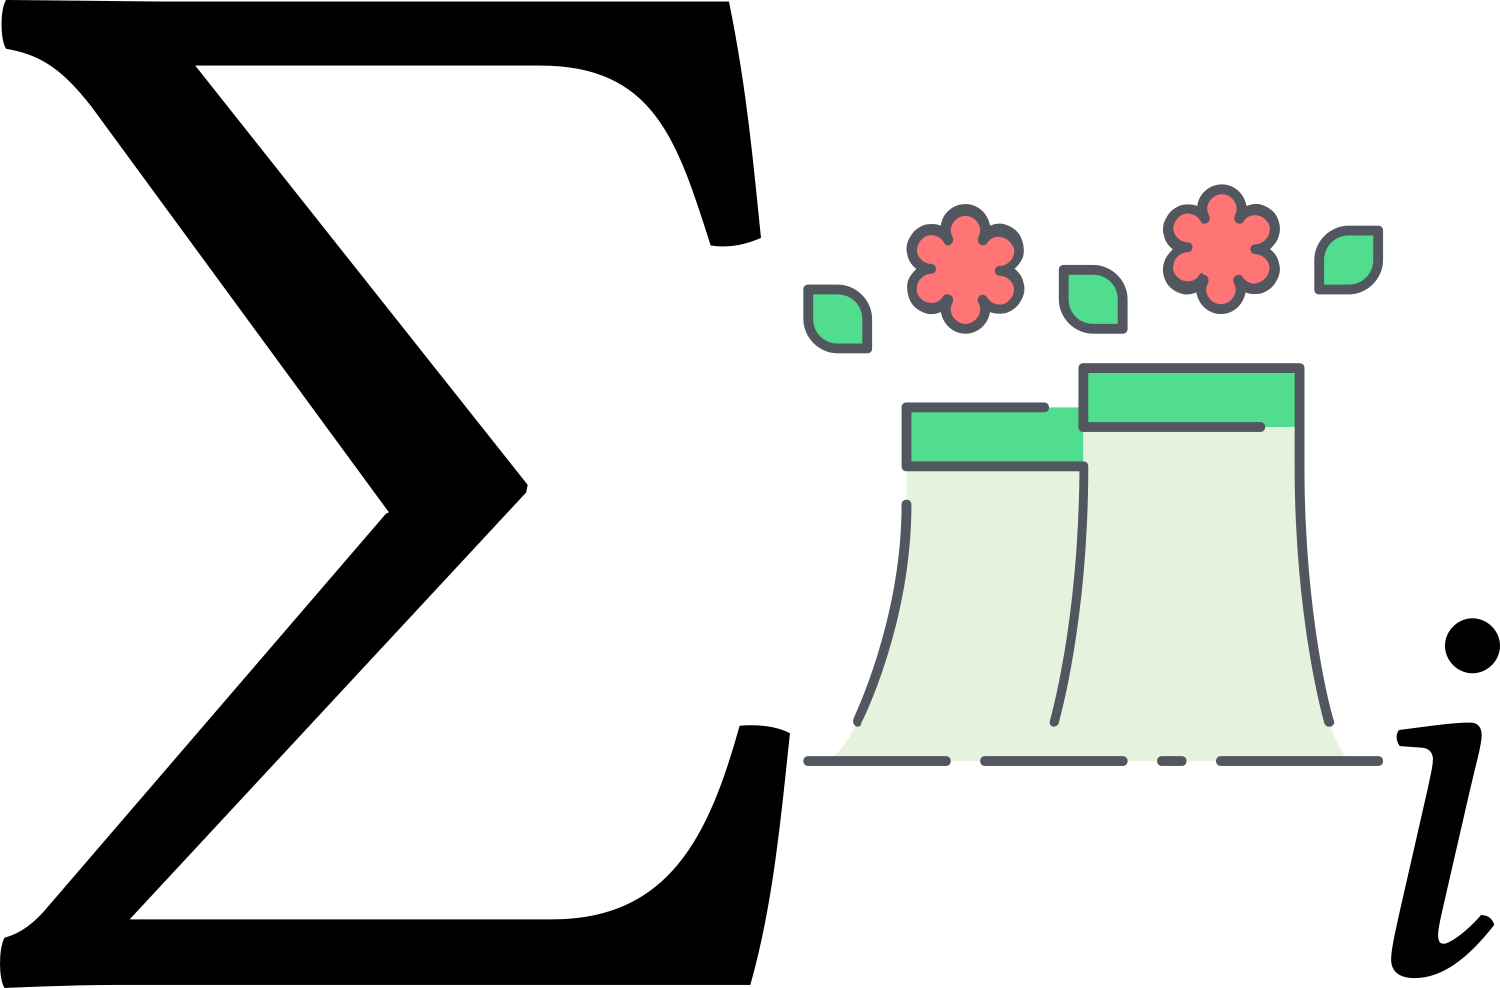
\includegraphics{logo} \end{center}

En el curso \textbf{Modelación matemática} aprenderemos a utilizar algunas herramientas matemáticas para analizar y entender los procesos de interés en ciencias ambientales. Los contenidos del índice se apegan al \href{Programa-curso.pdf}{programa completo del curso}, el cual se impartirá en los \href{Horario.pdf}{horarios normales establecidos}. Para conocer cuándo, cómo y qué temas se se impartirán puedes consultar la \href{Estrategia-docente.pdf}{estrategia docente}.

\hypertarget{criterios-de-evaluaciuxf3n}{%
\chapter{Criterios de evaluación}\label{criterios-de-evaluaciuxf3n}}

Las constribuciones a cada calificación parcial serán:

\begin{itemize}
\tightlist
\item
  Asistencia (25\%)
\item
  Trabajos de clase cumplidos (50\%)
\item
  Examen (25\%)
\item
  Participación (2 puntos extra máximo)
\end{itemize}

Cabe señalar, que la asistencia no corresponderá con su presencia en las sesiones sincrónicas, sino con el cumplimiento de los trabajos de clase. La participación se medirá tanto por participación directa en las sesiones sincrónicas como por el seguimiento que uds den a la clase por correo electrónico.

\hypertarget{cuxf3mo-se-daruxe1n-las-clases}{%
\section{¿Cómo se darán las clases?}\label{cuxf3mo-se-daruxe1n-las-clases}}

Trataré de apegarnos a los tiempos de actividades sincrónicas y asincrónicas establecidos en la \href{Estrategia-docente.pdf}{estrategia docente}, pero éstos son completamente flexibles. Una estrategia que me ha funcionado en cursos anteriores ha sido la de dedicar la última actividad sicrónica de la semana a resolver dudas, es en estas sesiones en las que hay muchas posibilidades de conseguir puntos de participación.

Todos los contenidos del curso, lecturas y presentaciones, se irán añadiendo a este sitio web conforme avanza el semestre. En el Google Classroom de la materia se irán anunciando las diferentes actividades y sesiones sincrónicas con anticipación suficiente. Igualmente, los examenes y resultados serán publicados a través de esta plataforma. A petición de uds, también se publicarán aquí los videos de las sesiones sincrónicas que tengamos, en especial para aquellos temas que sean mayor interés/dificultad/importancia. Los trabajos de práctica también se publicarán en Classroom.

Para finalizar, las clases sincrónicas estarán almacenadas en la playlist de la clase contenida en mi canal de youtube.

\hypertarget{reglas-del-saluxf3n}{%
\section{Reglas del salón}\label{reglas-del-saluxf3n}}

Estas, obviamente, son particulares del modelo en línea, por lo tanto aquí van las reglas de zoom:

\begin{enumerate}
\def\labelenumi{\arabic{enumi}.}
\tightlist
\item
  Micrófonos apagados
\item
  Cámaras prendidas, exceptuando:
  2.1. Si su velocidad de internet lo dificulta
  2.2. Si tienen datos limitados
\item
  Hacer muchas preguntas
\item
  Decirme si paso algo por alto
\end{enumerate}

\hypertarget{contacto}{%
\section{Contacto}\label{contacto}}

Para reportar fallos, resolver dudas y peticiones especiales grupales o individuales por favor enviar correo electrónico a \href{mailto:gerardo.mmc@enesmerida.unam.mx}{\nolinkurl{gerardo.mmc@enesmerida.unam.mx}}.

\hypertarget{unidad-i-modelos-determinuxedsticos}{%
\chapter{Unidad I: Modelos determinísticos}\label{unidad-i-modelos-determinuxedsticos}}

\hypertarget{introducciuxf3n-a-la-modelaciuxf3n}{%
\section{Introducción a la modelación}\label{introducciuxf3n-a-la-modelaciuxf3n}}

Imaginemos a seis personas invidentes, con la tarea de encontrar qué es el objeto que está frente a ellas usando únicamente el tacto. En la parábola de los seis hombres ciegos, el objeto es un elefante, de modo que la imágen que cada uno de ellos se forma del objeto depende enteramente de la parte del elefante que están tocando.

\begin{figure}

{\centering 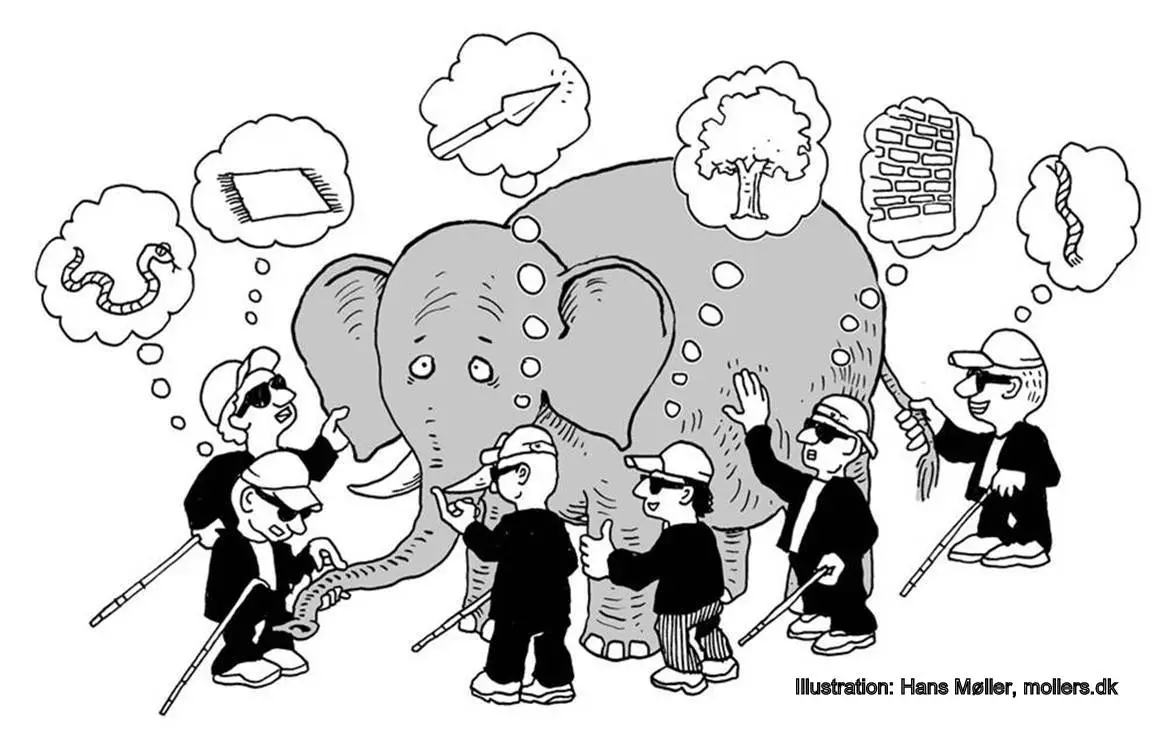
\includegraphics{Unidad-I/elefante} 

}

\caption{La parábola de los seis hombres ciegos inspeccionando un elefante.}\label{fig:unnamed-chunk-20}
\end{figure}

Quien toque los colmillos podrá pensar que se trata de una lanza, la trompa podría tratarse de una serpiente, la cola de una cuerda, las patas troncos de árbol y el cuerpo una pared. Es evidente que todas las hipótesis presentadas después de la inspección fueron erróneas, y que cuando estudiamos al mundo lo haremos igual, con la descripción de tan sólo una fracción de éste. Un séptimo hombre que pregunte a los otros seis qué fue lo que vieron podría formarse una imágen más completa del \emph{sistema} para proponer otra hipótesis: se trata de un objeto grande reposando sobre cuatro columnas con apéndices adelante y atrás.

Al estudiar los sistemas ecológicos, al igual que los ciegos, no sabremos que estamos frente a un elefante. Los sistemas ecológicos, al igual que los elefantes, también tienen componentes interconectados, y nosotros los ecólogos somos como los hombres ciegos, sólo podemos observar ciertas partes de los ecosistemas. En nuestro trabajo entonces, aprender a identificar y proponer hipótesis sobre cómo funcionan los sistemas ecológicos.

Las hipótesis propuestas por los seis hombres representan modelos, es decir simplificaciones del mundo que nos ayudan a entenderlo. Los modelos matemáticos son simplificaciones formales del mundo utilizando otro lenguaje, las matemáticas.

\hypertarget{funciones-buxe1sicas-y-su-representaciuxf3n-en-el-plano-cartesiano}{%
\section{Funciones básicas y su representación en el plano cartesiano}\label{funciones-buxe1sicas-y-su-representaciuxf3n-en-el-plano-cartesiano}}

\hypertarget{las-funciones}{%
\subsection{Las funciones}\label{las-funciones}}

En ciencias frecuentemente se estudia cómo un fenómeno afecta a otro. Por ejemplo, cómo la disponibilidad de recurso afecta el crecimiento poblacional. Estas relaciones pueden ser representadas matemáticamente utilizando el concepto de función. Una función es una regla de correspondencia entre dos conjuntos \(x\) y \(y\), de modo que para cada elemento del conjunto \(x\) existe un solo elemento del conjunto \(y\). Los elementos de \(y\) son llamados la imagen de \(x\) bajo la regla de correspondencia \(f\), que se denota como \(f(x)\). La función \(f(x)\) se lee \(f\) de \(x\), y el conjunto \(x\) es el \emph{dominio} y \(y\) es el \emph{codominio} de \(f\).

Debido a que todos los valores de \(y\) son producidos por la función \(f\), a \(x\) también se le conoce como variable independiente y a \(y\) como dependiente (puesto que depende de \(x\)). En términos prácticos \(f(x) = y(x)\).

En esta unidad estaremos hablando de funciones, concretamente de:

\begin{itemize}
\tightlist
\item
  Lineales
\item
  Cuadráticas
\item
  La curva normal
\item
  Trigonométricas
\end{itemize}

Para finalizar la unidad veremos una serie de aplicaciones de esta función, haciendo especial énfasis en la lineal.

\hypertarget{la-luxednea-recta}{%
\subsection{La línea recta}\label{la-luxednea-recta}}

Una línea recta se puede representar matemáticamente de varias maneras, la más común de ellas es por medio de una función. Una función, en cambio es una expresión matemática que indica una serie de operaciones (aritméticas por ejemplo), que serán aplicadas a un conjunto de números en sucesión (los números reales, p.~ej.) para producir otro conjunto. Así la, función lineal más sencilla puede ser:

\begin{equation}
    y(x) = x
\end{equation}

Lo que quiere decir que \(y\) es una función de \(x\), y cada valor de \(y\) será igual a cada valor de \(x\). En lenguaje matemático, el conjunto de números de \(x\) se llama el dominio, y \(y(x)\) el codominio. Algunas funciones lineales más complejas son:

\begin{equation}
    y(x) = ax
\end{equation}

donde \(a\) es una constante, lo que quiere decir que cada valor de \(y(x)\) será producido por el producto \(a \times x\). Finalmente, la expresión más común de una ecuación lineal es:

\begin{equation}
    y(x) = b + ax
\end{equation}

donde \(b\) también es una constante que se llama intercepto, y \(a\) es la pendiente, pues esta última determina la inclinación de la línea recta representada en el plano cartesiano.

\hypertarget{representaciones-gruxe1ficas-de-la-recta}{%
\subsubsection{Representaciones gráficas de la recta}\label{representaciones-gruxe1ficas-de-la-recta}}

Comencemos por dar un repaso del plano cartesiano. Este consiste de la representación de dos conjuntos de números reales en los que representamos una función, como una regla de correspondencia entre los valores de cada conjunto, de modo que a cada valor de \(x\) corresponde uno y sólo uno de los valores de \(y\). Cada conjunto se puede representar como una recta, y cuando éstas se disponen perperdiculares dan origen al plano.

\begin{figure}

{\centering 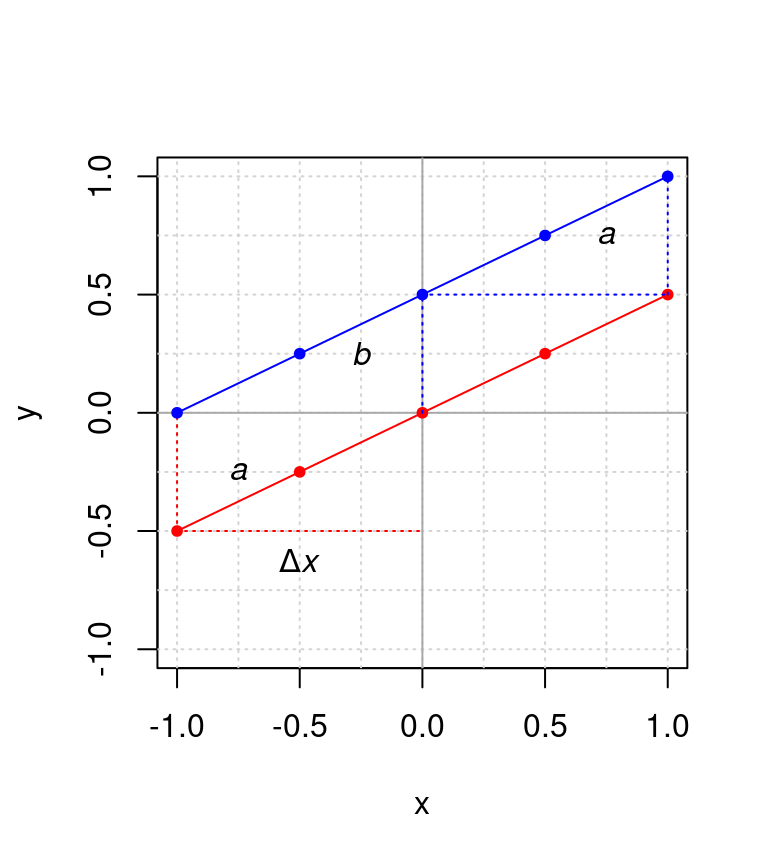
\includegraphics{Model-mate_files/figure-latex/unnamed-chunk-21-1} 

}

\caption{Ejemplo del plano cartesiado mostrando en rojo la correspondencia de valores para $y(x) = x$, donde los puntos corresponden a los pares de valores $(x = -1, y = -1), (-0.5, -0.5), (0, 0), (0.5, 0.5), (1, 1)$.}\label{fig:unnamed-chunk-21}
\end{figure}

Ahora veamos, con un ejemplo gráfico por qué la constante \(a\) recibe el nombre de \emph{pendiente}.

\begin{figure}

{\centering 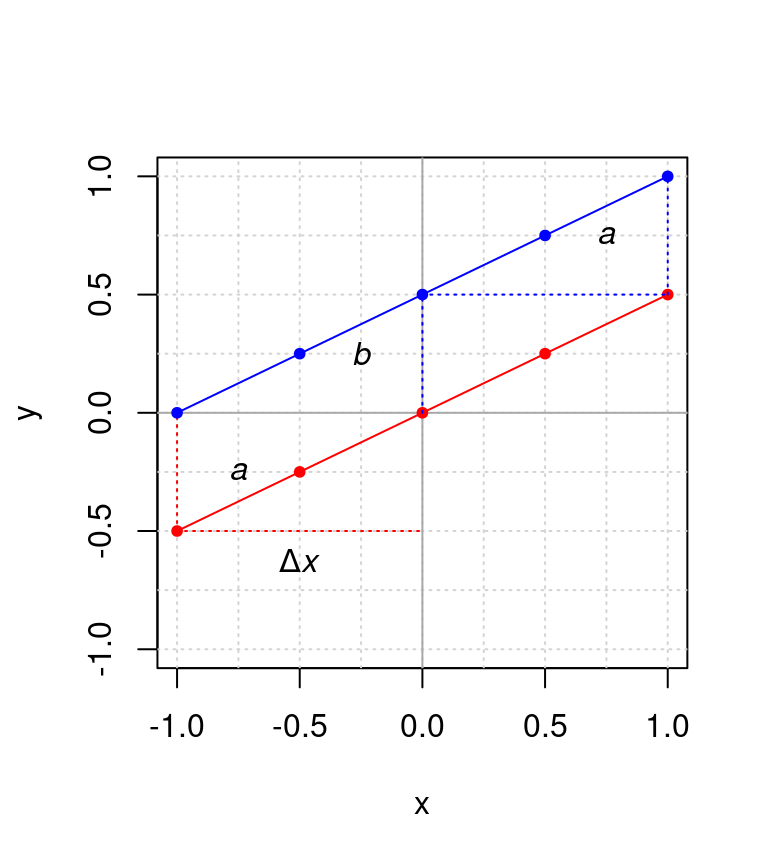
\includegraphics{Model-mate_files/figure-latex/unnamed-chunk-22-1} 

}

\caption{Gráficas de las funciones $y(x) = 0.5 x$ (en rojo) y $y(x) = 0.5 + 0.5 x$ (azul). Las líneas punteadas en colores indican el efecto de las constantes $a$ y $b$, mientas que Δ$x$ denota el cambio de una unidad de $x$.}\label{fig:unnamed-chunk-22}
\end{figure}

Como podemos ver, de manera más general, la línea recta es generada por una regla de correspondencia muy sencilla, un conjunto de valores \(X\) son multiplicados por un escalar \(a\), a los que se les puede añadir un \emph{intercepto} \(b\). El intercepto siempre es el valor de \(y(x)\) cuando \(x = 0\).

Ya se podrán imaginar que puede existir un sinnúmero de modelos lineales distintos, por ejemplo si \(y\) es una función de un gran número de conjuntos \(X\):

\begin{equation}
y(x_1, x_2, \dots, x_{n-1}, x_n) = b + a_1 x_1 + a_2 x_2 + \dots + a_{n-1} x_{n-1} + a_n x_n
\end{equation}

Gráficamente, estamos prácticamente limitados a explorar \(y(x_1, x_2)\), pero existen muchas herramientas matemáticas para entender modelos lineales más complejos que veremos más adelante. Estas herramientas y las implicaciones generales de la simplicidad del modelo lineal lo hacen uno de los modelos más útiles con que contamos para estudiar matemáticamente fenómenos dinámicos (que cambian de estado a lo largo del tiempo), como para estudiarlos de manera probabilística (con estadística). De hecho, el modelo lineal nos puede servir para entender modelos, como la parábola y el exponencial, que geométricamente no se parecen a la línea recta.

\hypertarget{la-paruxe1bola}{%
\subsection{La parábola}\label{la-paruxe1bola}}

Geométricamente, la parábola es muy distinta de la recta:

\begin{figure}

{\centering 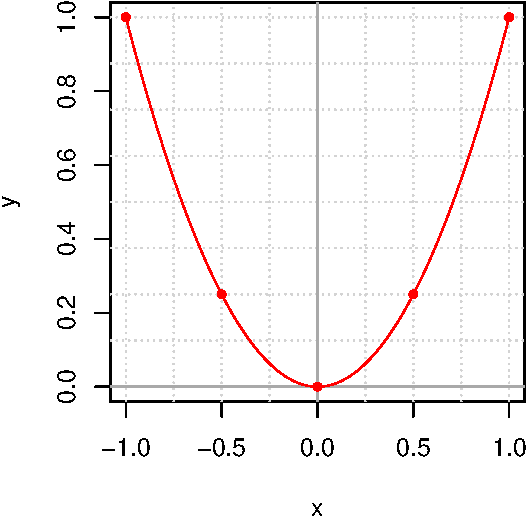
\includegraphics{Model-mate_files/figure-latex/parabola-1} 

}

\caption{Ejemplo del plano cartesiado mostrando en rojo la correspondencia de valores para $y(x) = x^2$, donde los puntos corresponden a los pares de valores $(x = -1, y = 1), (-0.5, 0.25), (0, 0), (0.5, 0.25), (1, 1)$.}\label{fig:parabola}
\end{figure}

La función matemática más sencilla que puede describir esta forma en el plano cartesiano es:

\begin{equation}
    y(x) = x^2
\end{equation}

Al igual que con los modelos lineales, las parábolas pueden representarse matemáticamente de otras formas más complejas:

\begin{itemize}
\tightlist
\item
  \(y(x) = a + bx + cx^2\)
\item
  \(y(x) = a + cx^2\)
\item
  \(y(x) = -x^2\)
\end{itemize}

Si uno es observador, se dará cuenta de que estas ecuaciones son muy similares a la recta, y es que es posible considerar que \(x^2\) se puede considerar como otro conjunto tal que \(x' = x^2\), resultando así en funciones perferctamente lineales:

\begin{itemize}
\tightlist
\item
  \(y(x) = a + bx + cx'\)
\item
  \(y(x) = a + cx'\)
\item
  \(y(x) = -x'\)
\end{itemize}

Entonce, lo que realmente distingue matemáticamente a una parábola de una recta, es la doble ocurrencia de cada valor de \(y\) para los distintos valores de \(x\):

\begin{figure}

{\centering 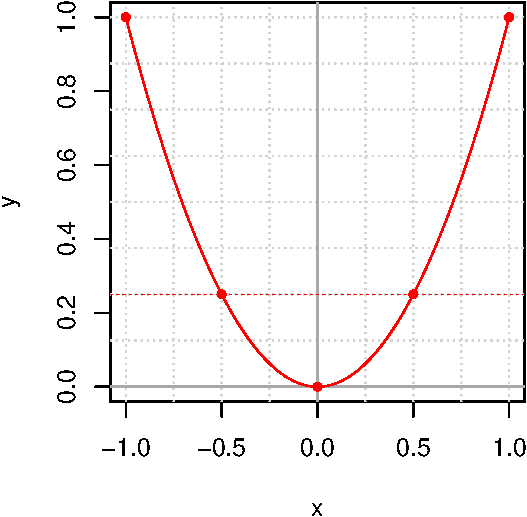
\includegraphics{Model-mate_files/figure-latex/parabola-2-1} 

}

\caption{Correspondencia de dos valores distintos de $x$ para el mismo valor de $y$}\label{fig:parabola-2}
\end{figure}

Cuando esto ocurre, las funciones tiene un solo punto a lo largo de todos los valores de \(x\), donde sólo va a ocurrir un valor único de \(y\). A estos puntos se les conocen como mínimos (par de valores con coordenadas \((0, 0)\) en la figura \ref{fig:parabola-2}). Los máximos, en cambio están ilustrados en la figura \ref{fig:parabola-3}, e igual corresponde al punto con coordenadas \((0, 0)\).

\begin{figure}

{\centering 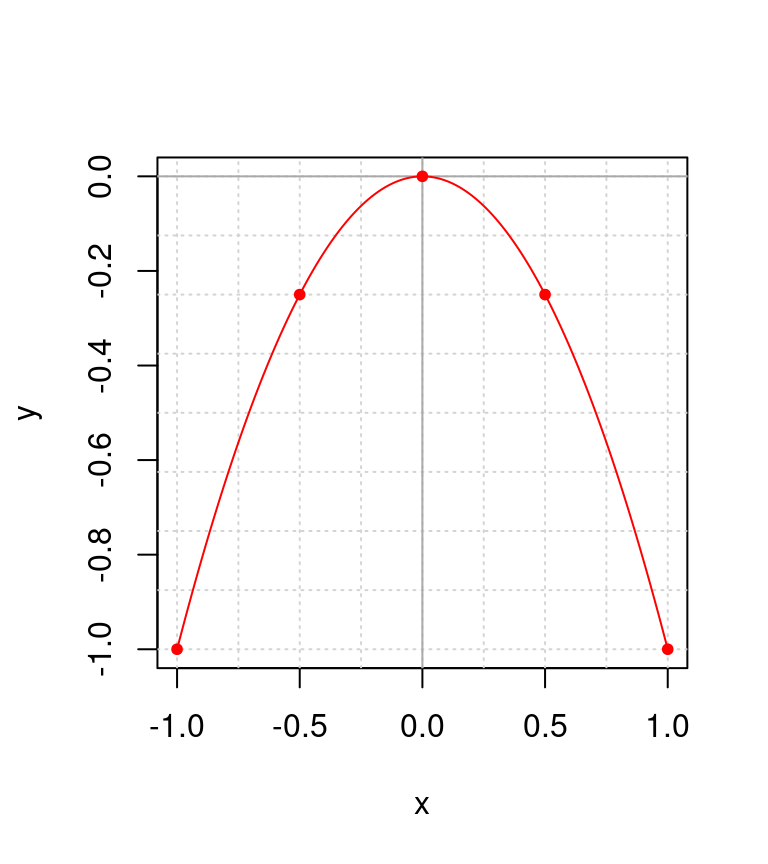
\includegraphics{Model-mate_files/figure-latex/parabola-3-1} 

}

\caption{Correspondencia de valores para $y = -x^2$.}\label{fig:parabola-3}
\end{figure}

En los modelos parabólicos más sencillos (\(y(x) = x^2, y(x) = -x^2\)), los puntos mínimos y máximos siempre estarán en las coordenadas \((x = 0, y = 0)\), pero es posible alterarlos. Por ejemplo en \(y(x) = 2 + x^2\), el mínimo estará en \((x = 0, y = 2)\). Para verificarlo resuelve \(y(x) = 2 + x^2\) para \(y(0)\), sustituyendo \(x\) por \(0\).

\hypertarget{ejercicio}{%
\subsubsection{Ejercicio}\label{ejercicio}}

A estas alturas, ya te podrás haber dado cuenta de ciertas propiedades de las parábolas, contesta las siguientes preguntas:

\begin{enumerate}
\def\labelenumi{\arabic{enumi}.}
\item
  ¿Qué tipo de punto único (mínimo o máximo) habrá en las siguientes parábolas?

  1.1. \(y(x) = 2 - x^2\)
  1.2. \(y(x) = 2x - 2x^2\)
  1.3. \(y(x) = 1 - x + 3x^2\)
  1.4. \(y(x) = x/2 - 4x^2/x\)
  1.5. \(y(x) = (5x)^2 - 3x + 1\)
\end{enumerate}

\hypertarget{cuxf3nicas}{%
\subsection{Cónicas}\label{cuxf3nicas}}

De manera muy general, una cónica es el conjunto de soluciones para una ecuación cuadrática cuando menos en dos variables. En este sentido, las parábolas, vistas en la sección anterior, son un tipo de cónica. Ejemplos:

\begin{enumerate}
\def\labelenumi{\arabic{enumi}.}
\tightlist
\item
  \(x^2 + y^2 = -1\)
\item
  \(x^2 + y^2 = 0\)
\item
  \(x^2 - y^2 = 0\)
\item
  \(xy - 1 = 0\)
\item
  \(x^2 - y = 0\)
\end{enumerate}

Debido a la generalidad de la definición de \emph{cónicas}, las ecuaciones 1-5 tienen una variedad de formas muy distintas, en comparación con las secciones de rectas y parábolas (Figura \ref{fig:conicas}). La mayoría de estas forman surgen como solución a la intersección de un plano bidimensional con una línea rotando sobre un eje definido dentro de ella en un espacio tridimencional (\href{https://www.mathplanet.com/Oldsite/media/28029/conic.png}{ver ejemplo})

\begin{figure}

{\centering 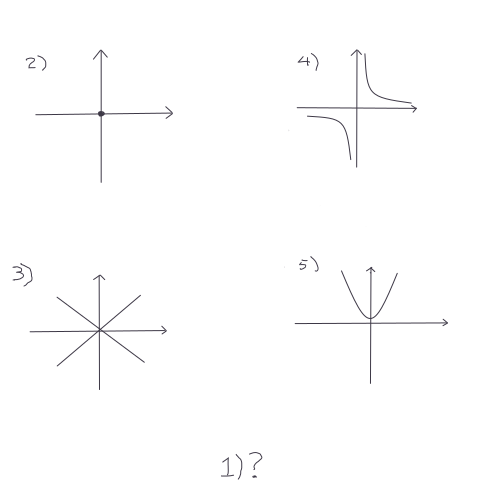
\includegraphics{Unidad-I/conicas} 

}

\caption{Representación gráfica de las ecuaciones 1-5.}\label{fig:conicas}
\end{figure}

\hypertarget{la-curva-normal}{%
\subsection{La curva normal}\label{la-curva-normal}}

En el curso de probabilidad y estadística, se acordarán, se mencionó repetidamente a la distribución normal. En cuestión de matemáticas, la distribución normal puede ser representada como una ecuación:

\begin{equation}
    y(x) = \frac{1}{\sigma \sqrt{2\pi}}e^{-\frac{(x-\mu)^2}{2\sigma^2}} \label{eq:normal}
\end{equation}

donde \(\mu\) es la media aritmética, \(\sigma^2\) es la varianza y \(x\) son todos los valores de la variable que observamos. Cuando tenemos datos de un experimento y los analizamos haciendo el cálculo del promedio estimamos justamente a \(\mu\) de la ecuación \eqref{eq:normal}, y al estimar la varianza obtenemos a \(\sigma^2\) de la misma ecuación. Como es importante notar, al hacer estos cálculos estamos asumiendo que nuestros datos tienen una distribución (un histograma) que puede ser descrita por la ecuación \eqref{eq:normal}.

Como vimos en la sección de parábolas, las funciones que no son monótonas (los valores de \(y\) no aumentan o disminuyen a lo largo de \(x\)), tienen un punto máximo o mínimo. La curva normal, tiene propiedades similares, aunque debido a la presencia de la función exponencial (\(e^{\dots}\)), los valores de \(y(x)\) \textbf{siempre serán positivos}. Por lo tanto, la curva normal tiene un punto máximo que corresponde a \(y(\mu)\), o sea, \(y\) alcanza su punto máximo cuando \(x=\mu\) (Figura \ref{fig:normal}).

\begin{figure}

{\centering 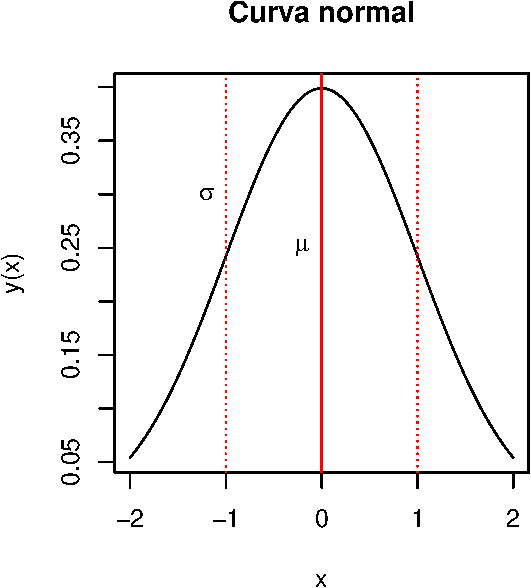
\includegraphics{Model-mate_files/figure-latex/normal-1} 

}

\caption{Representación gráfica de la curva normal.}\label{fig:normal}
\end{figure}

En estadística, esta función representa en el eje de las \(y\) la \emph{densidad} de la variable \(x\). Densidad se refiere a la proporción de observaciones de \(x\) dentro de un intervalo definido de \(x\). Por lo tanto, la curva normal, representa la probabilidad de observar ese valor de \(x\), de ahí que \(\mu\) sea el valor teórico más probable. En lo que respecta a \(\sigma^2\), éste representa qué tan concentrados estarán los valores de \(x\) alrededor de \(\mu\). Altos valores de \(\sigma\) se traducirán en baja concentración alrededor de \(\mu\) (Figura \ref{fig:vari}).

\begin{figure}

{\centering 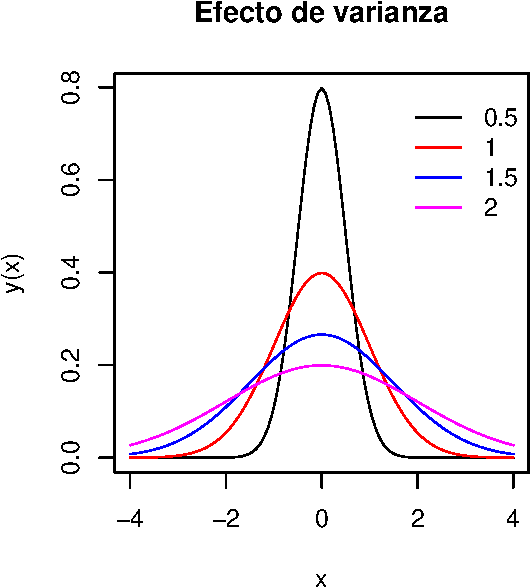
\includegraphics{Model-mate_files/figure-latex/vari-1} 

}

\caption{Efecto de  la varianza sobre la la dispersión alrededor de la media.}\label{fig:vari}
\end{figure}

\hypertarget{funciones-trigonomuxe9tricas}{%
\section{Funciones trigonométricas}\label{funciones-trigonomuxe9tricas}}

En esta sección revisaremos algunas de las funciones trigonométricas y cómo se representan en el plano cartesiano.

La trigonometría es una rama de las matemáticas que se comenzó a desarrollar a partir de la necesidad de medir distancias de manera indirecta. Por ejemplo, la distancia entre la luna y la tierra y la tierra y el sol, la distancia entre dos barcos, la distancia entre un barco y el puero más cercano. Las herramientas trigonométricas entonces se comenzaron a desarrollar utilizando la geometría de triángulos rectángulos. Aquí es preciso describir el teorema de los triángulos proporcionales, dados dos triángulos con ángulos internos idénticos y longitudes de lados diferentes, los cocientes de las longitudes de sus lados serán iguales (Figura \ref{fig:trian-prop}).

\begin{figure}

{\centering 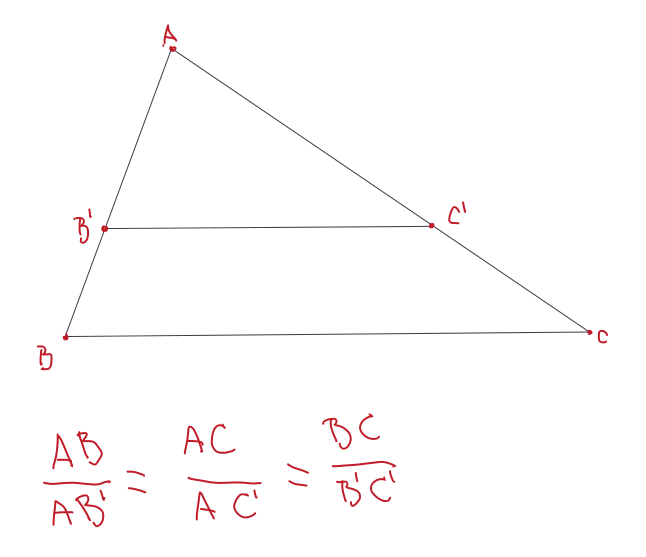
\includegraphics{Unidad-I/Trian-prop} 

}

\caption{El teorema de los ángulos proporcionales es la base para las fórmulas geométricas de las funciones trigonométricas.}\label{fig:trian-prop}
\end{figure}

De modo que sin importar las longitudes de los lados, los cocientes de las longitudes siempre serán iguales, lo cual se puede extender a todos los triángulos rectángulos, la base geométrica para la trigonometría. Aquí veremos entonces las funciones trognométricas básicas seno, coseno y tangente.

\hypertarget{nomenclatura-de-triuxe1ngulos-para-trigonometruxeda-buxe1sica}{%
\subsubsection{Nomenclatura de triángulos para trigonometría básica}\label{nomenclatura-de-triuxe1ngulos-para-trigonometruxeda-buxe1sica}}

Hay una serie de términos tradicionales que se emplean en trigonometría, los cuales utilizaremos a lo largo del curso. Se trata de los nombres que se dan a los lados y ángulos internos de un triángulo rectángulo. Por lo general, el triángulo rectángulo lo interpretaremos como una representación del plano cartesiano, de modo que los \textbf{catetos} corresponden a los ejes de las \(x\) y \(y\), y son los lados que forman un ángulo recto al cruzarse. El lado que los une en secante, es la \textbf{hipotenusa}. El ángulo que forma la hipotenusa con el eje de las \(x\) tradicionalmente recibe el nombre con la letra griega \(\theta\) (teta).

\begin{figure}

{\centering 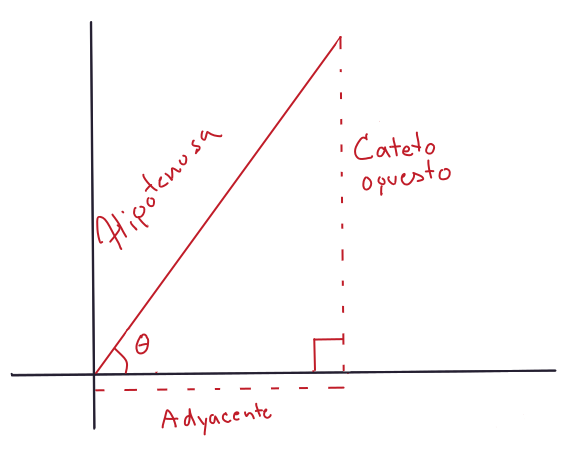
\includegraphics{Unidad-I/nomenclatura} 

}

\caption{Representación gráfica de las partes del triángulo y los nombres que reciben tradicionalmente en trigonometría plana.}\label{fig:nomen-trig}
\end{figure}

\hypertarget{las-funciones-trigonomuxe9tricas-buxe1sicas}{%
\subsubsection{Las funciones trigonométricas básicas}\label{las-funciones-trigonomuxe9tricas-buxe1sicas}}

Todas las funciones trigonométricas representan una descripción del ángulo \(\theta\) como el cociente de la longitud de dos lados del triángulo rectángulo de modo que:

\begin{enumerate}
\def\labelenumi{\arabic{enumi}.}
\tightlist
\item
  \textbf{Seno}: \(\sin(\theta) = \frac{\mathrm{Opuesto}}{\mathrm{Hipotenusa}}\)
\item
  \textbf{Coseno}: \(\cos(\theta) = \frac{\mathrm{Adyacente}}{\mathrm{Hipotenusa}}\)
\item
  \textbf{Tangente}: \(\tan(\theta) = \frac{\mathrm{Opuesto}}{\mathrm{Adyacente}}\)
\end{enumerate}

Para recordar las fórmulas de cada función podemos utilizar la mnemotecnia:

\begin{itemize}
\tightlist
\item
  \textbf{Seno}: SOH (Seno, Opuesto, Hipotenusa)
\item
  \textbf{Coseno}: CAH (Coseno, Adyacente, Hipotenusa)
\item
  \textbf{Tangente}: TOA (Tangente, Opuesto, Adyacente)
\end{itemize}

\hypertarget{representaciuxf3n-gruxe1fica-de-las-funciones-trigonomuxe9tricas}{%
\subsubsection{Representación gráfica de las funciones trigonométricas}\label{representaciuxf3n-gruxe1fica-de-las-funciones-trigonomuxe9tricas}}

Para entender por qué las funciones trigonométricas se comportan como lo hacen es útil tener en cuenta que representan el cociente de dos números que cambian uno en relación del otro. Esto queda de manifiesto en la Figura \ref{fig:catetos}. Como se puede apreciar, la hipotenusa (\(H\) en la misma figura) se mantiene constante, pues representa el radio de la circunferencia, mientras que los catetos se alargan o encojen conforme la hipotenusa se acerca a los ejes \(x\) o \(y\).

\begin{figure}

{\centering 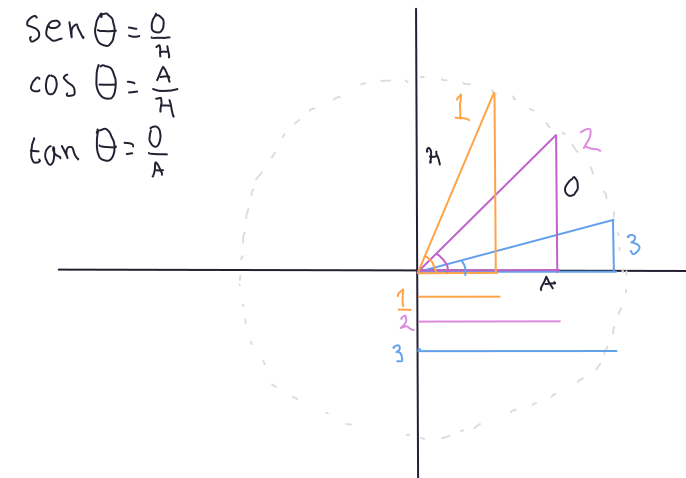
\includegraphics{Unidad-I/Func-trigo} 

}

\caption{Representación gráfica del efecto del ángulo sobre la longitud de los catetos.}\label{fig:catetos}
\end{figure}

Como es de esperarse, los valores del seno y coseno están limitados por 1 y -1 cuando la longitud del cateto es igual a la hipotenusa. La tangente, por otro lado, puede tomar valores que van de \(-\infty, +\infty\) cuando el cateto adyacente tiene longitud cero \(0\). Aquí, mediremos los ángulos en radianes, o unidades de \(\pi\), donde \(\pi = 180°\)

\begin{figure}

{\centering 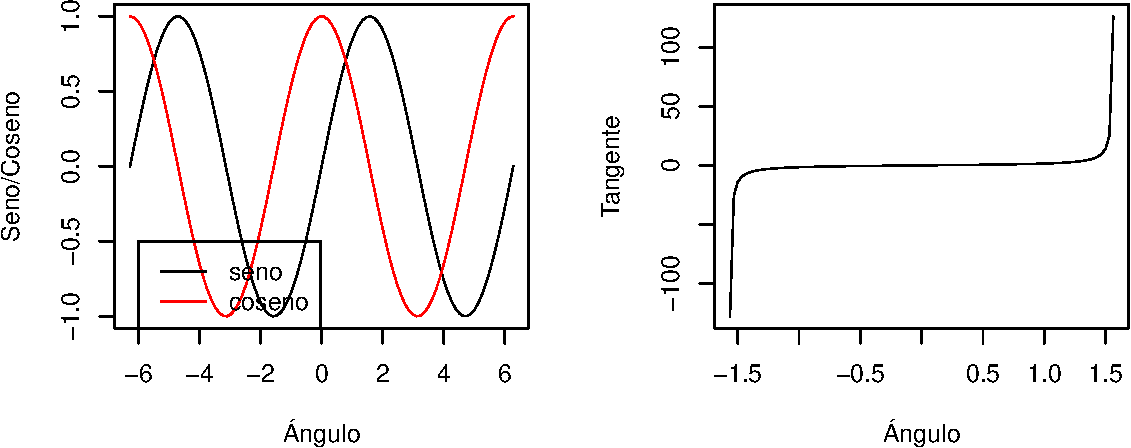
\includegraphics{Model-mate_files/figure-latex/graf-trig-1} 

}

\caption{Gráfica de las funciones trigonométricas básicas.}\label{fig:graf-trig}
\end{figure}

Las funciones seno, coseno y tangente son las básicas en trigonometría. Otras funciones comunes, pasadas en la inversión de las mecionadas son la secante, cosecante y cotangente respectivamente. Al igual que otras operaciones aritméticas, para las funciones trigonométricas, existen inversiones. La inversión de una multiplicación es una divisón, de la suma es la resta, del exponente es la raíz. Las inversiones de las funciones trigonométricas reciben el nombre de Arco-\(f(\theta)\), de modo que al aplicarlas al resultado de la función obtenemos el valor del ángulo:

\begin{enumerate}
\def\labelenumi{\arabic{enumi}.}
\tightlist
\item
  \(\theta = \arcsin \left(\frac{0}{H}\right)\)
\item
  \(\theta = \arccos \left(\frac{A}{H}\right)\)
\item
  \(\theta = \arctan \left(\frac{O}{A} \right)\)
\end{enumerate}

\hypertarget{aplicaciones-de-las-funciones-trigonomuxe9tricas}{%
\subsubsection{Aplicaciones de las funciones trigonométricas}\label{aplicaciones-de-las-funciones-trigonomuxe9tricas}}

En mi experiencia, las dos funciones con más aplicaciones en modelación de sistemas ambientales son la tangente y el coseno. Para comenzar, la tangente de un ángulo tiene una relación directa con la pendiente de una recta. Si recordamos la recta está descrita por la ecuación:

\begin{equation}
    y = a + bx \label{eq:lin-2}
\end{equation}

donde \(b\) es la pendiente de la recta que se forma al graficar \(x\) y \(y\) en el plano cartesiano. En realidad \(b\) es la tangente del ánguo que se forma entre la recta y el eje de las \(x\). Por lo tanto, cuando nos encontramos ante un modelo formulado por medio de ecuaciones diferenciales, por ejemplo, lo valores que obtenemos al hacer los cálculos de ese sistema es una pendiente o tangente.

El coseno, por otro lado, nos es muy útil para forzar la oscilación de algún parámetro. Ello es necesario cuando estamos interesados en representar fenómenos cíclicos como la temperatura diaria o anual. En la práctica, podemos reemplazar la pendiente \(b\) de la ecuación \eqref{eq:lin-2} por una función coseno.

\begin{figure}

{\centering 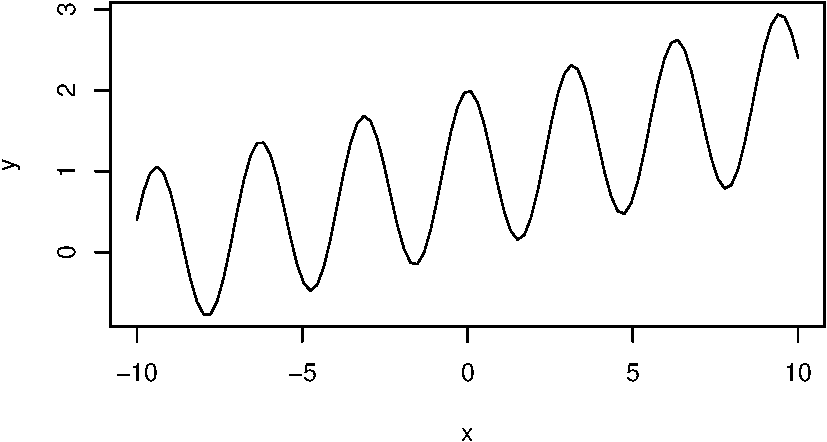
\includegraphics{Model-mate_files/figure-latex/coseno-forz-1} 

}

\caption{Gráfica de la función $y = 2 cos(x)^2 + 0.1  x$.}\label{fig:coseno-forz}
\end{figure}

\hypertarget{la-luxednea-recta-como-modelo-universal}{%
\section{La línea recta como modelo ``universal''}\label{la-luxednea-recta-como-modelo-universal}}

De los modelos vistos anteriormente, la línea recta es el más flexible y común de todos. Por su simplicidad, puede ser utilizado para representar muchos fenómenos de la naturaleza, incluso aquellos cuyo comportamiento es\ldots{} !no lineal¡

Cuando decimos no lineal, nos referimos, generalmente, a los casos en que una regla de correspondencia entre \(x\) y \(y\) representada en el plano cartesiano no forman una línea recta. Ya hemos visto que, matemáticamente, es posible concebir como lineales reglas de corresondencia que geométricamente no son lineales, de ahí que la línea recta sea tan flexible. Para que una ecuación sea considerada como lineal debe cumplir con las siguientes características:

\begin{enumerate}
\def\labelenumi{\arabic{enumi}.}
\tightlist
\item
  Sólo hay adición de variables
\item
  Sólo hay multiplicación con constantes
\item
  Las variables solo están elevadas a la potencia 1
\end{enumerate}

Con base en estas definiciones, las siguientes ecuaciones \textbf{no} son lineales

\begin{enumerate}
\def\labelenumi{\arabic{enumi}.}
\tightlist
\item
  \(xy = 1\)
\item
  \(y = a + b x^2\)
\item
  \(y = e^x\)
\end{enumerate}

Aún cuando estas expresiones no son lineales, es posible transformar algunas de ellas para que adquieran propiedades lineales. Para comenzar, el caso 1, no puede ser linealizado. Para el caso 2, ya vimos un transformación posible, si asumimos que existe una \(x'\) tal que \(x' = x^2\). Para el caso 3 hay que usar un poco más de conocimiento de dos funciones matemáticas, el logaritmo y la exponencial.

\hypertarget{el-logaritmo}{%
\subsection{El logaritmo}\label{el-logaritmo}}

Para entender cómo funciona la transformación logarítmica, revisemos qué hace el logaritmo. Supongamos que queremos encontrar el valor de la incógnita \(x\) en la siguiente ecuación:

\[10^x = 20\]
La operación necesaria para invertir el radical \(10^x\) y encontrar el valor de \(x\) es precisamente el logaritmo base 10, de modo que:

\[\log_{10} 10^x = \log_{10} 20\]
\[x \log_{10} 10 = \log_{10} 20\]
sabemos que \(\log_{10} 10 = 1\) pues \(10^1 = 10\) por lo que:

\[x = \log_{10} 20 \approx 1.3\]
Así como en esta ocasión utilizamos \(\log_{10}\) (logaritmo base 10), se puede utilizar como base cualquier número \(b > 0\), si está en el conjunto de los números reales (positivos). El logaritmo más común recibe el nombre de natural, que utiliza de base la constante \(e = 2.718282 ...\) de Euler. La convención en escritura de logaritmos es:

\begin{itemize}
\tightlist
\item
  Logaritmo natural: \(\ln\)
\item
  Logaritmo base 10: \(\log\)
\item
  Logaritmo base \(b > 0, b \in \mathbb{R}\): \(\log_b\)
\end{itemize}

Aún cuando esta es la convención más común, en la modelación, la mayoría de las veces que se utiliza \(\log\) se refiere a \(\ln\), de modo que a menos que se especifique la base, \(\log\) y \(\ln\) también significan \(\log_e\).

\hypertarget{la-funciuxf3n-exponencial}{%
\subsection{La función exponencial}\label{la-funciuxf3n-exponencial}}

Una de las funciones más comunes en aplicaciones matemáticas es la exponencial que se denota por \(\exp(x)\), que significa \(e^x\). De este modo cuando \(y\) es una función exponencial de \(x\), tenemos que:

\[y(x) = \exp(x) = e^x\]
La función exponencial puede tomar formas más complejas, por ejemplo, conteniendo una ecuación lineal:

\[y(x) = \exp(a + bx) = e^{a + bx}\]
y dadas las reglas de los exponentes, también es equivalente a:

\[y(x) = e^a e^{bx} = a' e^{bx}\]

\hypertarget{linealizando-la-funciuxf3n-exponencial}{%
\subsubsection{Linealizando la función exponencial}\label{linealizando-la-funciuxf3n-exponencial}}

Como se ha mostrado en esta sección, transformar una función exponencial en lineal es relativamente sencillo. En sentido literal, las transformaciones logaritmicas no son lineales sino log-lineales pues:

\begin{equation}
    y(x) = e^{a + bx} \label{eq:expon}
\end{equation}

se convierte en:

\begin{equation}
    \log y(x) = a + bx \label{eq:log-lin}
\end{equation}

donde el lado izquierdo es una función logarítmica y el derecho es estrictamente lineal. Matemáticamente entonces, la transformación es lineal \(\forall x \in \mathbb{R}\), puesto que \(\log y\) puede tomar cualquier valor entre \(-\infty\) y \(+\infty\). Entonces, la ecuación número 3 de la lista de ecuaciones no-lineales al principio de esta sección es:

\[\log y(x) = \ln y(x) = x\]

Esta equivalencia, como veremos más adelante y como verán en modelación estadística, es sumamente útil en la modelación de sistemas dinámicos.

\hypertarget{representaciuxf3n-gruxe1fica-de-la-funciuxf3n-exponencial}{%
\subsubsection{Representación gráfica de la función exponencial}\label{representaciuxf3n-gruxe1fica-de-la-funciuxf3n-exponencial}}

En la función exponencial, la variable \(y\) crece muy rápido. De hecho, su crecimiento en cualquier punto es proporcional al valor que tiene en ese punto. Es decir que si tomamos un punto cualquiera en \(y\) y dibujamos una tangente a ese punto, la pendiente de esa recta tendrá el mismo valor que \(y\).

\begin{figure}

{\centering 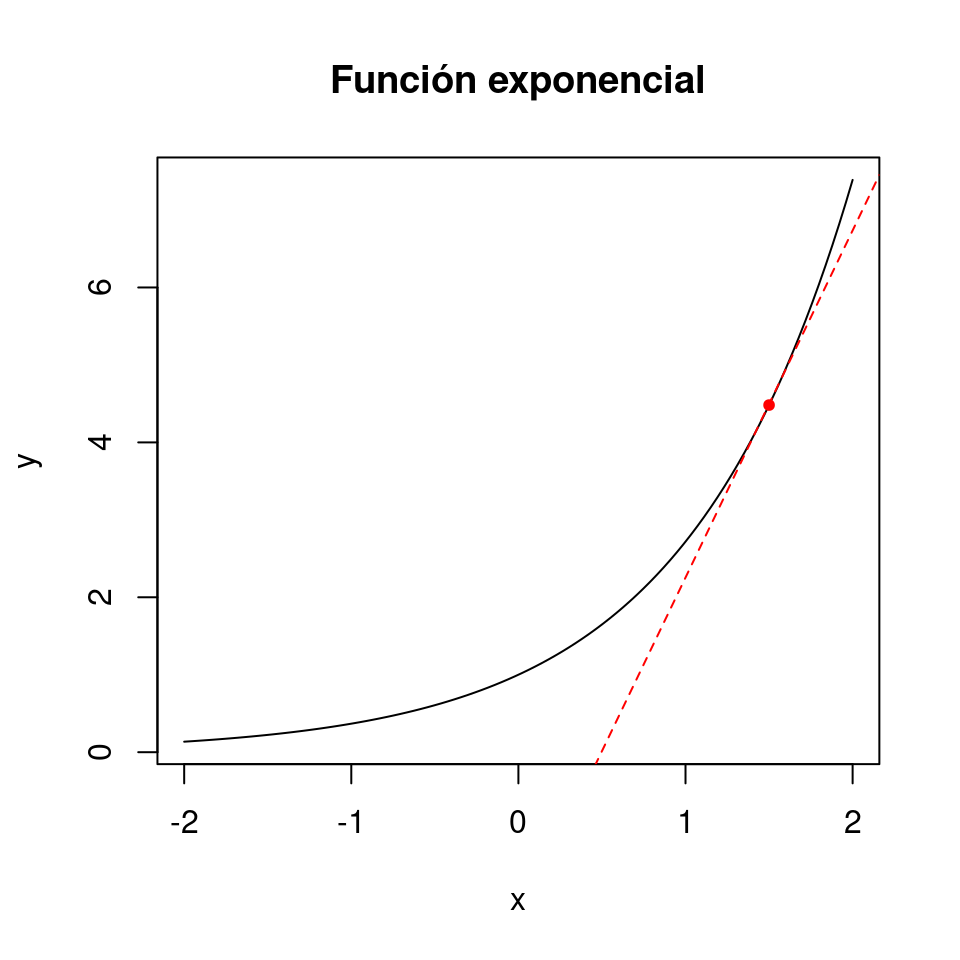
\includegraphics{Model-mate_files/figure-latex/expon-1} 

}

\caption{Representación gráfica de la función exponencial. El punto rojo representa y = exp(1.5), de modo que la pendiente de la recta tangente a la curva (en rojo) en ese punto es precisamente exp(1.5).}\label{fig:expon}
\end{figure}

Esta relación entre el valor de la curva y la pendiente tiene implicaciones importantísimas en modelación de poblaciones, pues expone las razones por las cuales el crecimiento demográfico puede ser descrito como \emph{exponencial}: el crecimiento neto de una población, el total de individuos nuevos que se incorporarán a la población, en ese instante es proporcional al número de individuos repoductivos de esa población. Es por esta razón que el número total de individuos que nacen en una población es más grande cuantos más individuos haya, a pesar de que la tasa reproductiva por unidad de tiempo sea la misma.

Veamos como ejemplo, que el crecimiento de la humanidad, desde que se pueden obtener estimaciones, es aproximadamente exponencial \ref{fig:popn-wd}.

\begin{figure}

{\centering 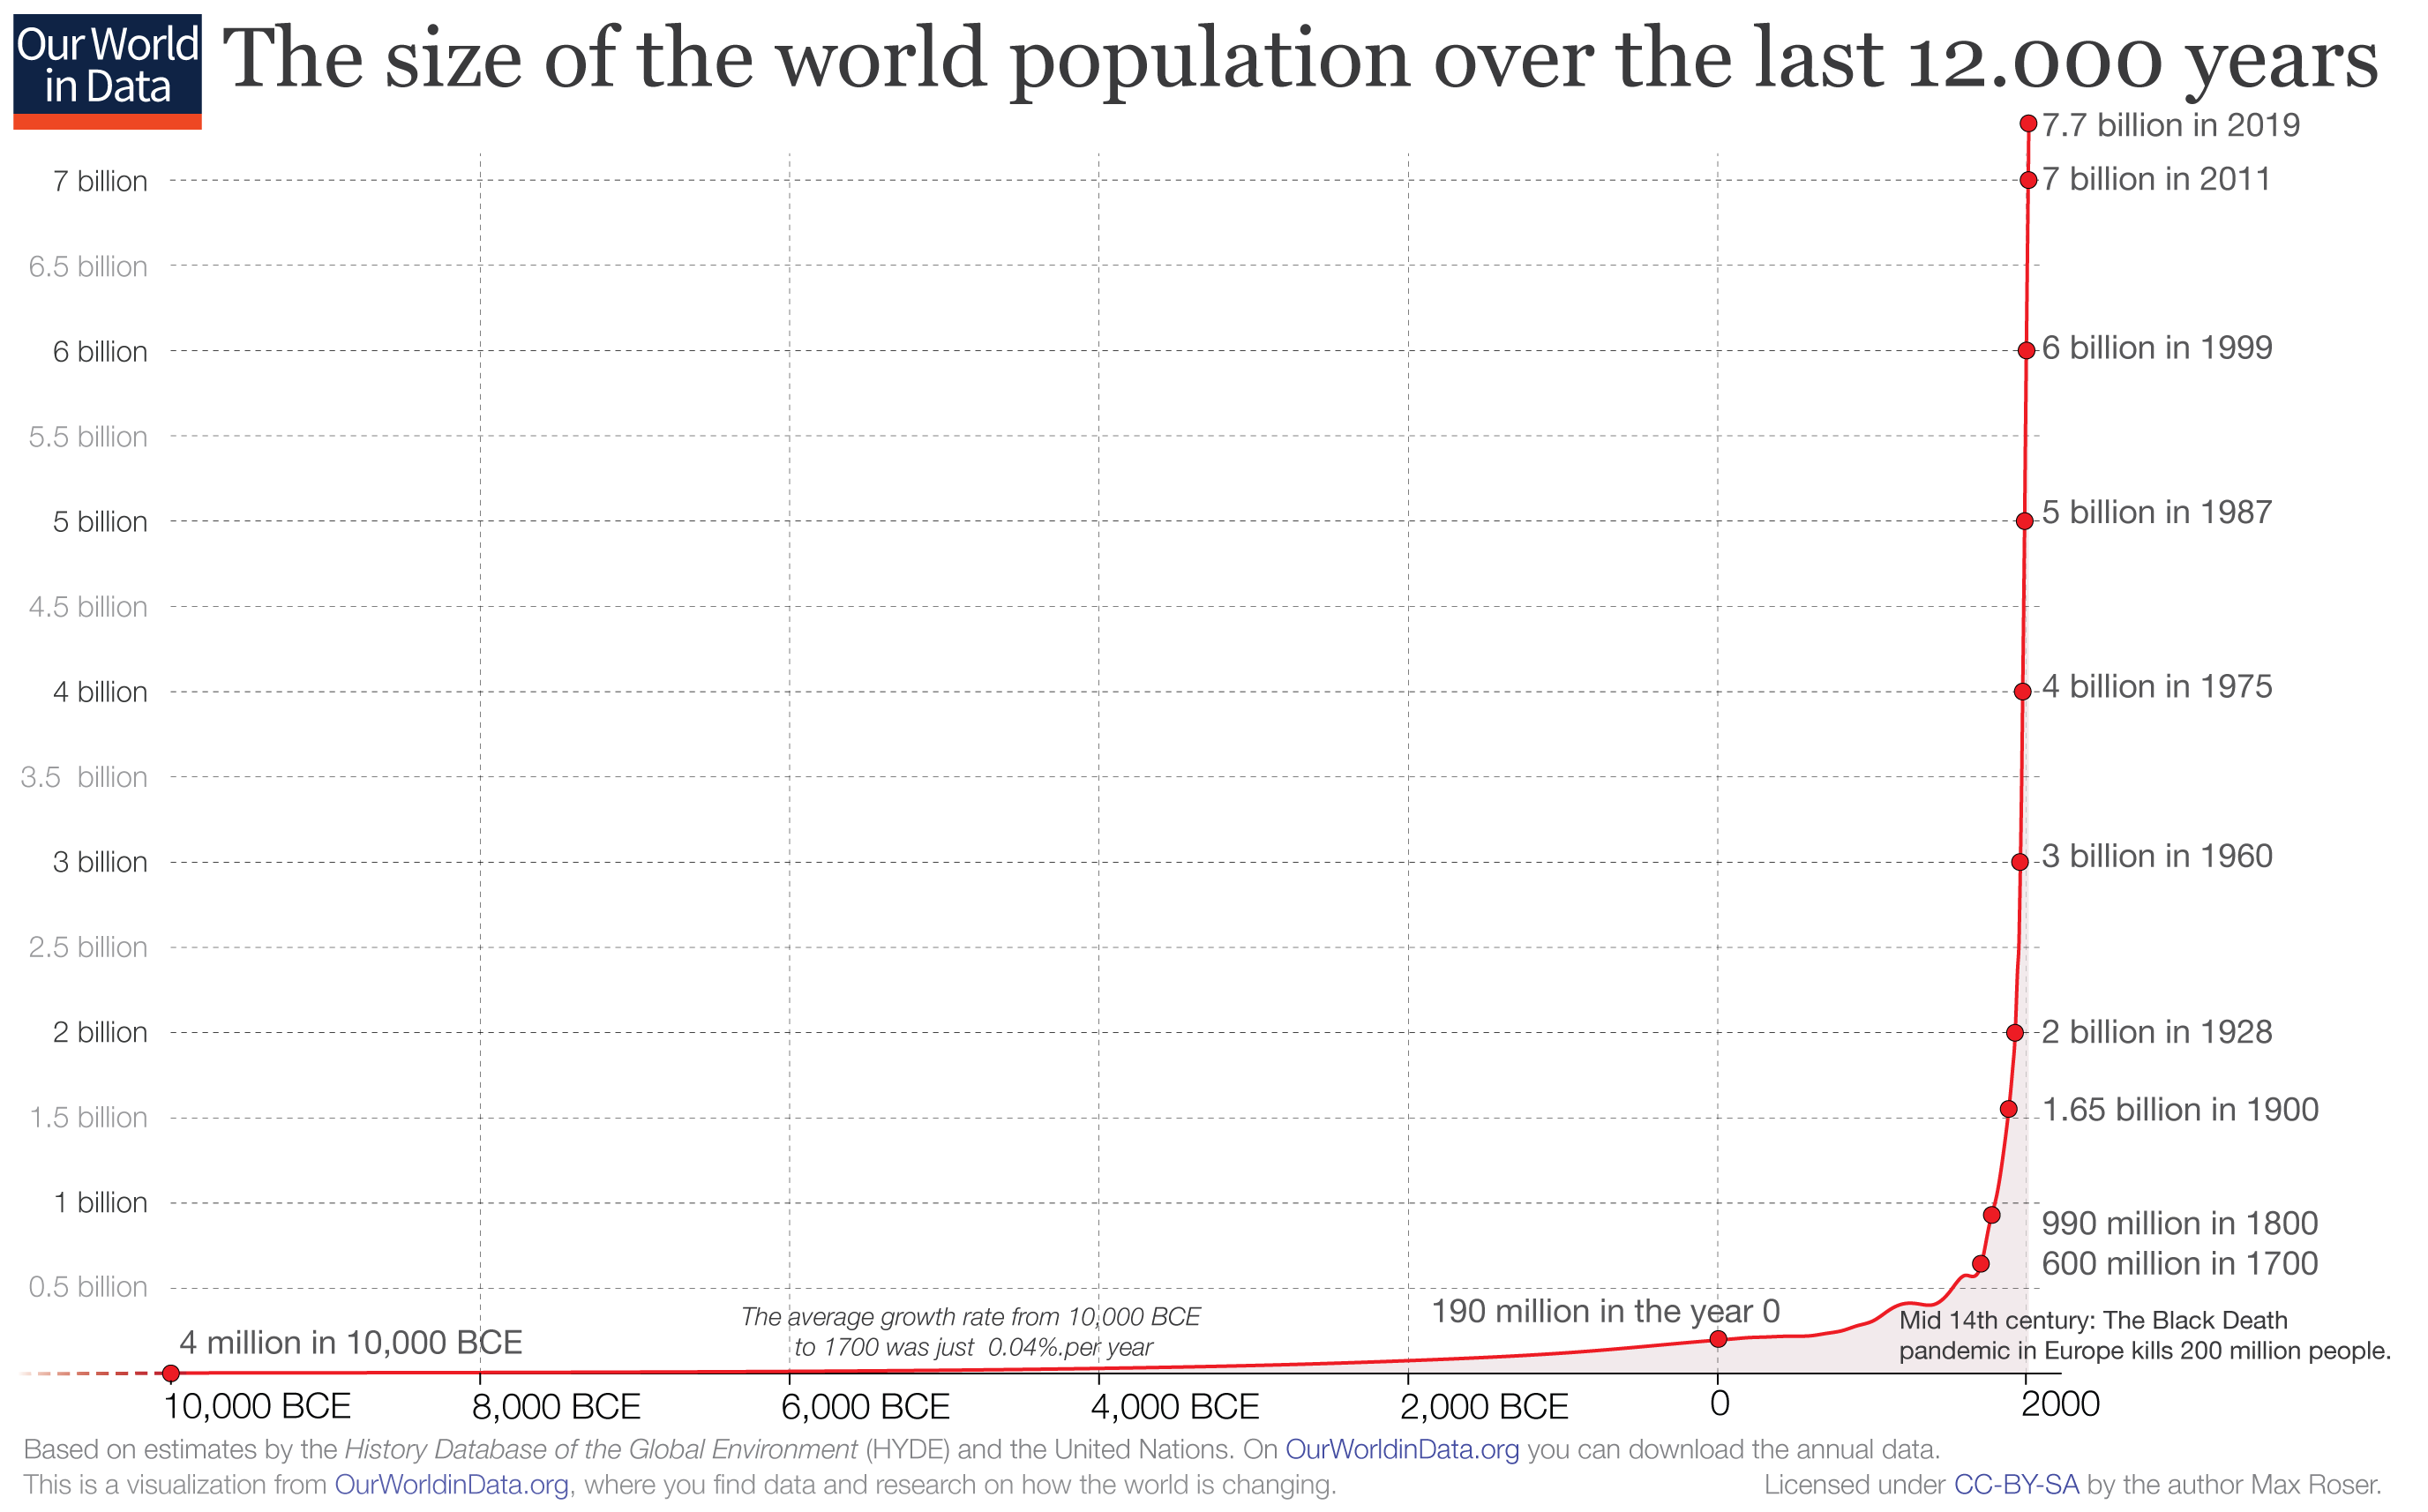
\includegraphics{Unidad-I/popn} 

}

\caption{Población humana a lo largo del tiempo, según estimaciones de [Our world in data](https://ourworldindata.org/world-population-growth).}\label{fig:popn-wd}
\end{figure}

A diferencia del ejemplo de la figura \ref{fig:expon}, donde \(y = \exp(x)\), para representar el crecimiento de la población humana tenemos que medir la tasa reproductiva, de modo que podamos establecer la relación directa entre el tiempo y el tamaño de la población. En otras palabras, medir cuántos individuos son producidos en promedio por cada individuo presente en la población en cada unidad de tiempo:

\begin{equation}
N(t) = \exp(r \cdot t) \label{eq:poblac}
\end{equation}

donde \(r\) es la tasa reproductiva de la población y utilizamos \(N\) en lugar de \(y\) para representar al \(N\)úmero de individuos, y \(t\) en lugar de \(x\) para dejar claro que \(x\) representa tiempo. Si utilizamos el conocimiento de la subsección anterior, veremos que al aplicar el logaritmo a ambos lados de la ecuación \eqref{eq:poblac} obtenemos ¡una ecuación lineal!

\begin{equation}
    \log N = r \cdot t
\end{equation}

Es evidente que un modelo tan sencillo como este tiene serias deficiencias biológicas. Por ejemplo, cuando \(t = 0\), \(\exp(r \cdot t) = 1\), de modo que se asume que siempre habrá cuando menos un individuo presente. Esto puede o no ser cierto, por lo que una forma más generalizable incluye un intercepto para el tamaño poblacional inicial:

\begin{equation}
    N(t) = N_0 e^{r \cdot t} \rightarrow \log N(t) = \log N_0 + r \cdot t
\end{equation}

\hypertarget{representaciuxf3n-gruxe1fica-del-logaritmo}{%
\subsubsection{Representación gráfica del logaritmo}\label{representaciuxf3n-gruxe1fica-del-logaritmo}}

A diferencia de la función exponencial, donde el crecimiento de \(y\) es cada vez más \emph{rápido}, en el logaritmo es más lento (figura \ref{fig:log}).

\begin{figure}

{\centering 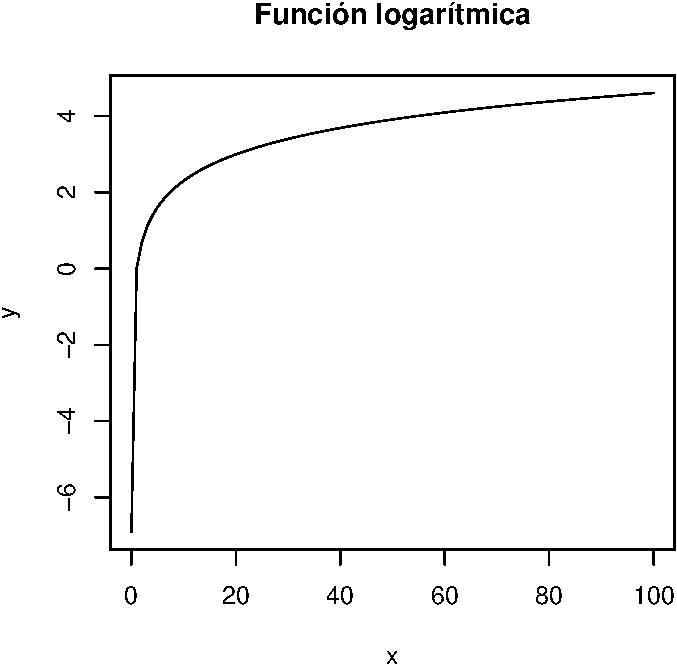
\includegraphics{Model-mate_files/figure-latex/log-1} 

}

\caption{Representación gráfica del logaritmo con y = log x.}\label{fig:log}
\end{figure}

\hypertarget{relevancia-de-la-recta}{%
\subsection{Relevancia de la recta}\label{relevancia-de-la-recta}}

Una vez cubiertas las funciones logarítmicas y exponenciales, hemos comenzado a vislumbrar la relevancia más amplia de la recta para fenómenos que no son lineales. En el cálculo diferencial, la recta nos da los elementos para entender el significado de la derivada, y también es el bloque fundamental para implementar métodos de integración numérica relativamente sencillos, para ecuaciones diferenciales que no se pueden integrar analíticamente.

\hypertarget{modelaciuxf3n-de-sistemas-sociales-y-ambientales}{%
\section{Modelación de sistemas sociales y ambientales}\label{modelaciuxf3n-de-sistemas-sociales-y-ambientales}}

\hypertarget{tipos-generales-de-modelos}{%
\subsection{Tipos generales de modelos}\label{tipos-generales-de-modelos}}

De manera muy general, un modelo es una representación miniatura del sistema que nos interesa estudiar. Así que podemos representar los sistemas socioambientales mediante modelos:

\begin{enumerate}
\def\labelenumi{\arabic{enumi}.}
\tightlist
\item
  Diagramáticos: Dibujos, bosquejos, gráficos
\item
  Conceptuales: Descripciones verbales o escritas
\item
  Físicos: Maquetas que repliquen aspectos importantes del sistema de estudio
\item
  Formales: Ecuaciones matematicas que nos permitan cuantificar el fenómeno a partir de observaciones, o análisis simbólico.
\end{enumerate}

Las diferentes herramientas matemáticas que hemos revisado representan los bloques para construir representaciones matemáticas de los fenómenos que se estudian en ciencias ambientales.

De todas las herramientas que vimos la línea recta es el más útil de todos pues nos permite entender el concepto de pendiente, y representar funciones más complejas como una colección de rectas. Por otra parte, fenómenos como el crecimiento poblacional que es exponencial se puede representar como una línea recta en escala logarítmica.

El modelo exponencial lo utilizaremos para modelar fenómenos cuyo etado en el futuro se verá afectado por su estado actual, tal como el número de individuos nuevos en el futuro en una población depende del número de individuos que actualmente contiene. Modelos como el lineal, se pueden en cambio utilizar para representar fenómenos cuyo estado futuro es independiente de su estado actual (en cierta medida). Veamos una serie de ejemplos.

\hypertarget{consumo-eluxe9ctrico-en-ciudades}{%
\subsection{Consumo eléctrico en ciudades}\label{consumo-eluxe9ctrico-en-ciudades}}

Aunque existen muchos factores sociales, económicos y culturales que explican el consumo de electricidad en una ciudad, el número de habitantes puede considerarse uno de los factores más importantes. De modo que, si en México el ciudadano promedio consume 2157 kWh anualmente (datos de OCDE), el consumo de una ciudad puede asumirse como el producto de sus habitantes y el consumo promedio:

\[\mathrm{kWh} = N \times \mathrm{Consumo\ promedio} \]

\begin{figure}

{\centering 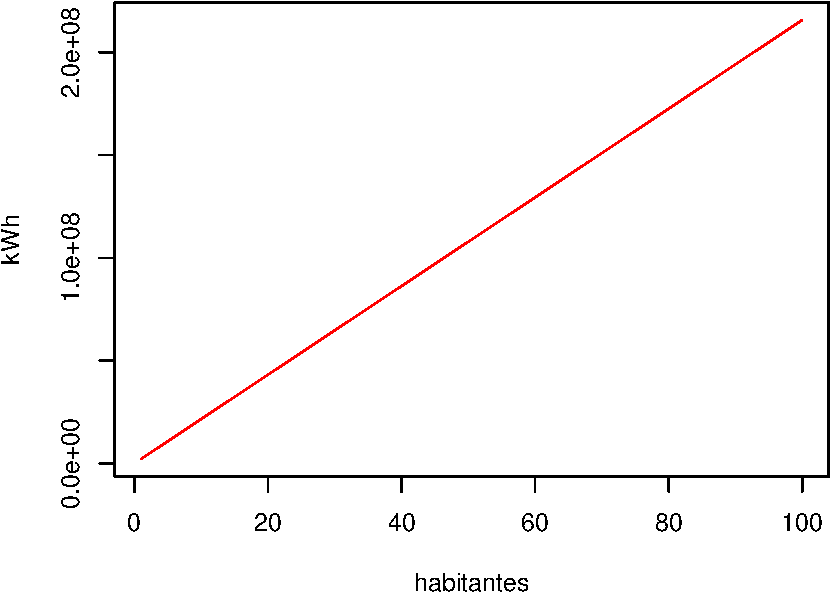
\includegraphics{Model-mate_files/figure-latex/electr-1} 

}

\end{figure}

\hypertarget{crecimiento-de-una-poblaciuxf3n}{%
\subsection{Crecimiento de una población}\label{crecimiento-de-una-poblaciuxf3n}}

La cantidad de individuos nuevos en una población depende de la cantidad de individuos presentes. Por lo tanto, este fenómeno se puede representar con una función exponencial:

\begin{equation}
N(t) = N_0e^{rt} \label{eq:crec-pobl}
\end{equation}

donde \(N\) es el número de individuos, \(N_0\) es el tamaño inicial de la población, \(r\) es la tasa de crecimiento (proporción de indiciduos nuevos en cada unidad de tiempo), y \(t\) es el tiempo. Aquí he reemplazado \(N\) por \(y\) y \(t\) por \(x\).

Como ya sabemos, el modelo exponencial, lo podemos transformar a una línea recta:

\[ \ln N = \ln N_0 + rt\]

por lo tanto si observamos el curso de una población a lo largo del tiempo, y no se forma una línea recta, podemos concluir que la tasa \(r\) no ha sido constante, tal como ocurre con la población del mundo (\ref{fig:tasa-crec}).

\begin{figure}

{\centering 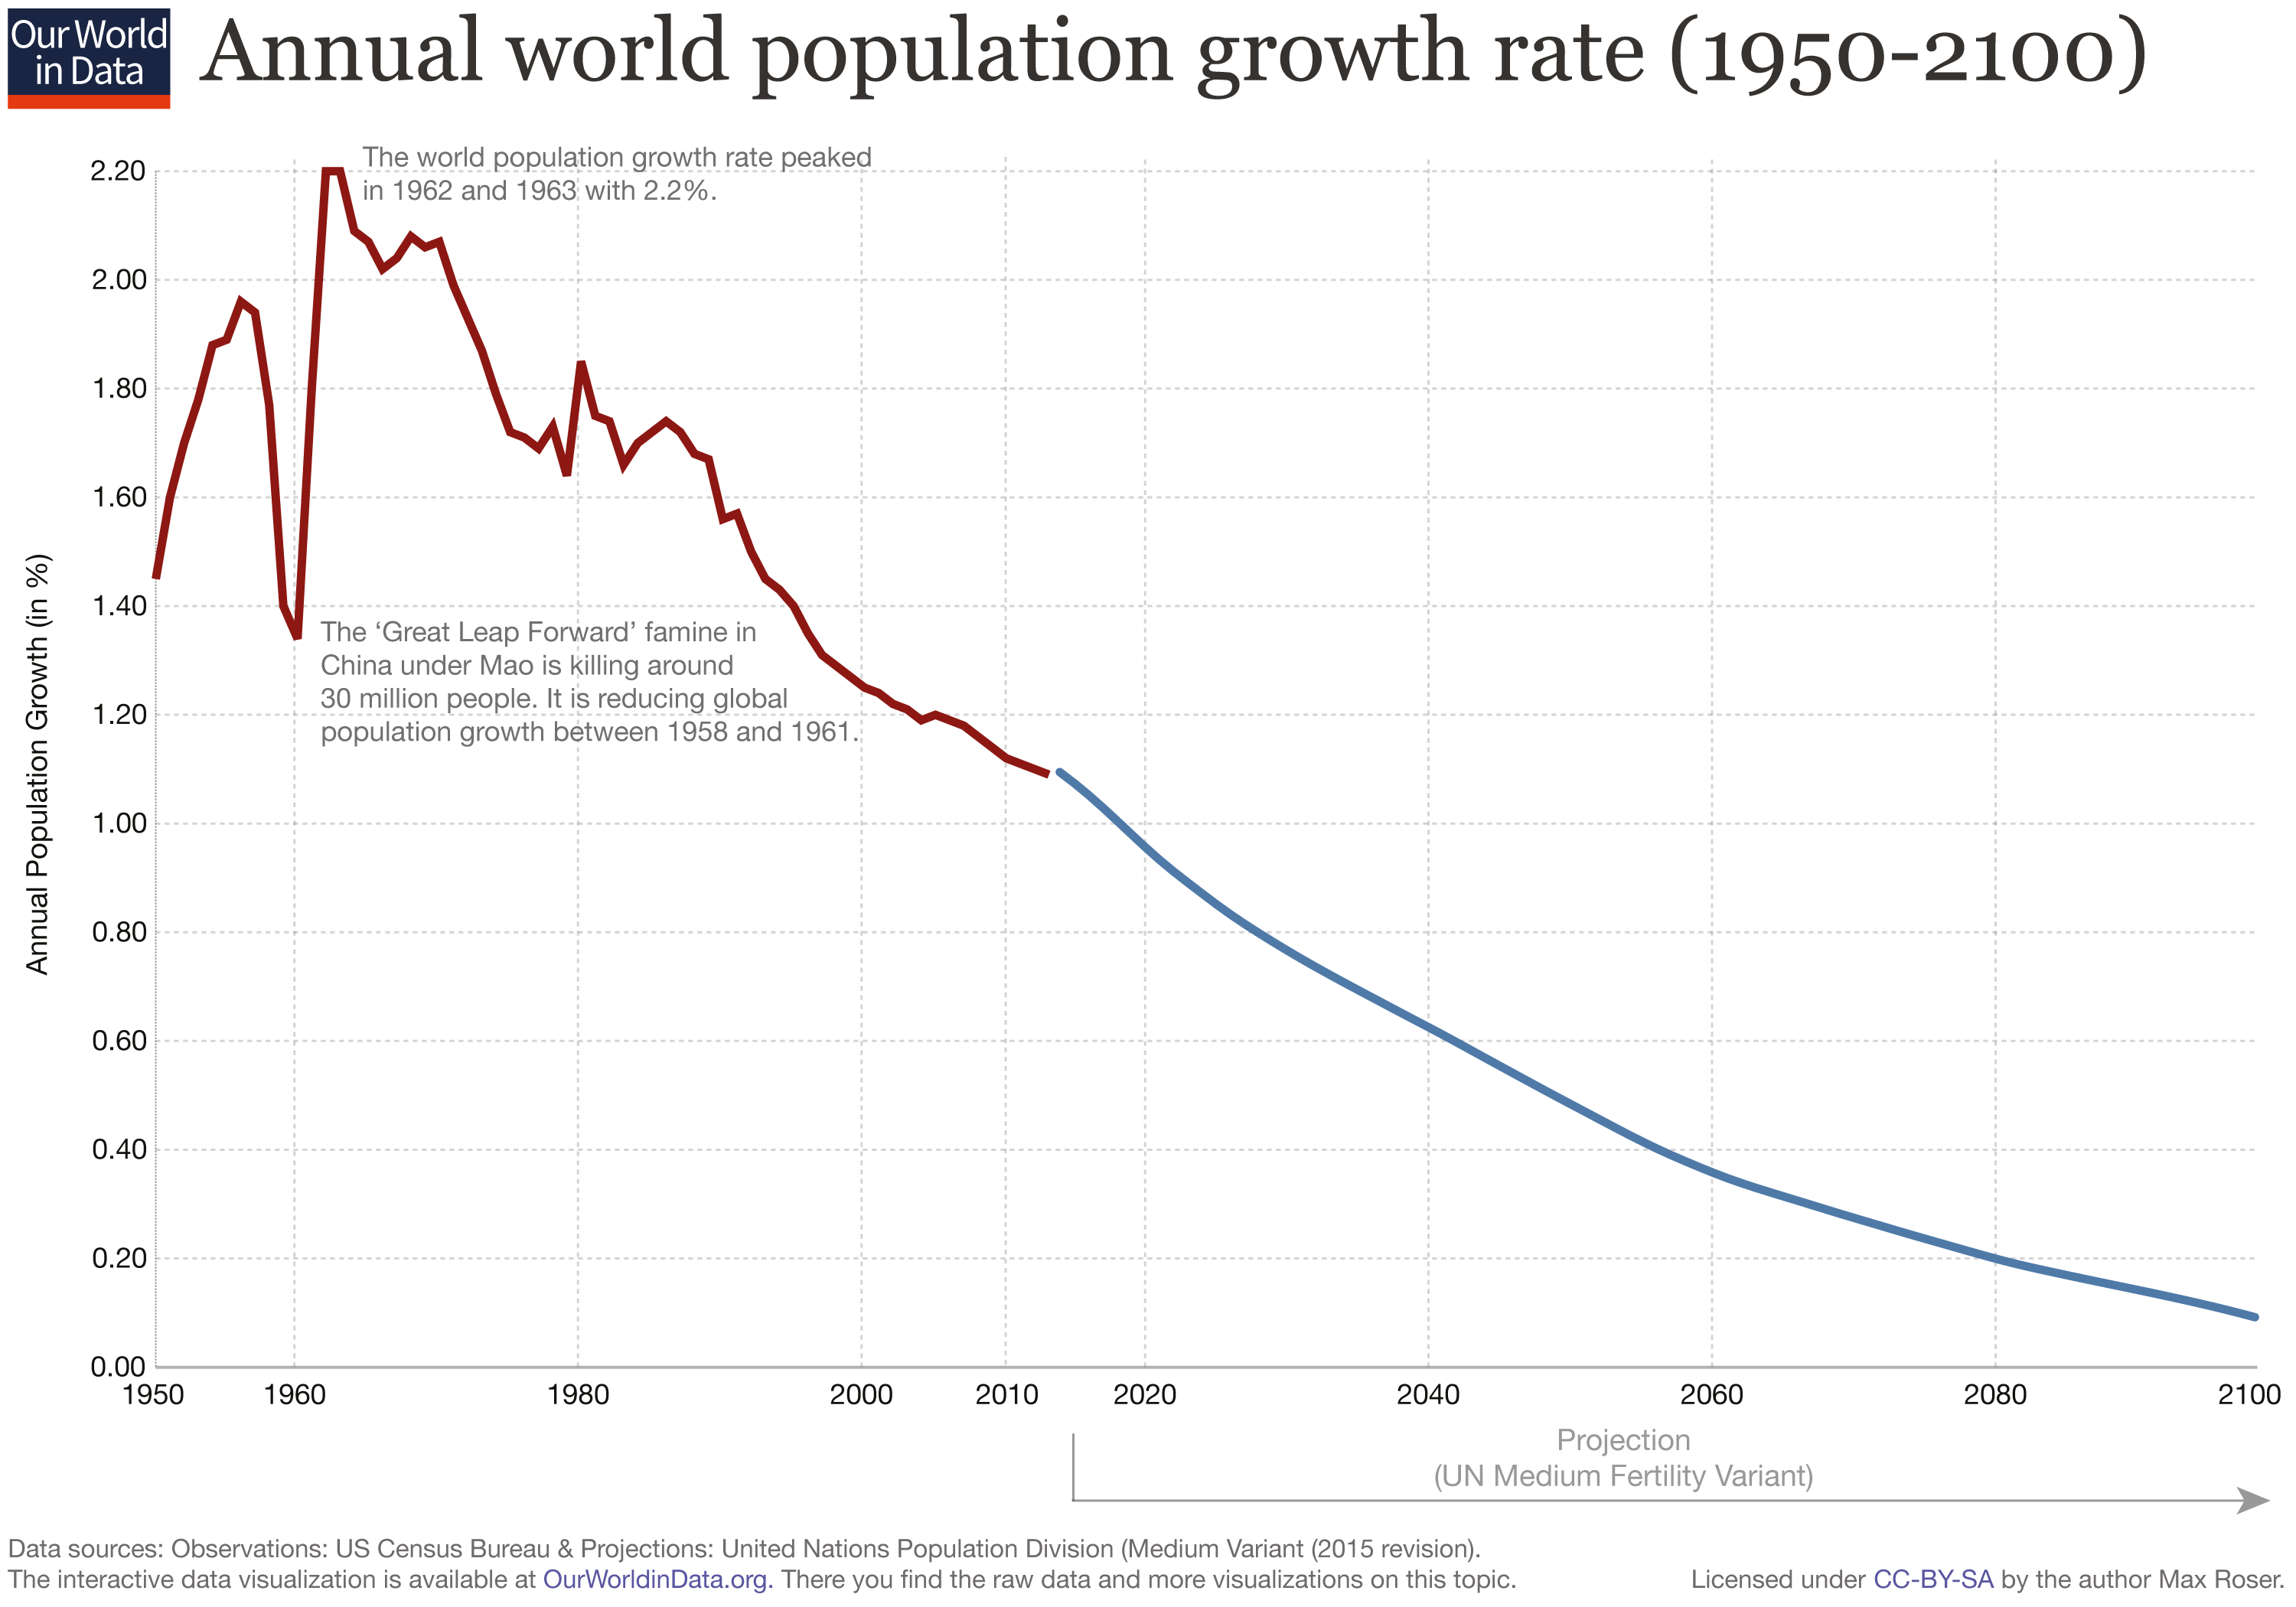
\includegraphics{Unidad-I/Tasa-crec} 

}

\caption{Cambios históricos y proyectados de la tasa de crecimiento de la población humana.}\label{fig:tasa-crec}
\end{figure}

Bajo este escenario, un trabajo interesate para un científico hambiental sería estudiar las causas de las variaciones históricas de \(r\), transformándolo de una cantidad fija, como se asume en la
ecuación \eqref{eq:crec-pobl} a una función de otros factores como la disponibilidad de alimento:

\[r(\mathrm{alimento}) = a + b \mathrm{\ alimento} + c \mathrm{\ alimento}^2\]

Conforme avancemos en el semestre aprenderemos a usar matemáticas más sofisticadas que nos permitirán concebir los sistemas socio-ambientales de un modo dinámico.

\hypertarget{modelos-deterministas}{%
\subsection{Modelos deterministas}\label{modelos-deterministas}}

Todos los modelos que vimos a la fecha:

\begin{enumerate}
\def\labelenumi{\arabic{enumi}.}
\tightlist
\item
  Línea recta
\item
  Parábola
\item
  Cónicas
\item
  Curva normal
\item
  Trigonométricas
\end{enumerate}

Se consideran modelos deterministas, lo que quiere decir que siempre que los resolvamos producirán el mismo resultado. La contraparte de los modelos deterministas son los modelos \textbf{estocásticos}, que con ayuda de una computadora producirán resultados ligeramente diferentes cada vez que los resolvamos.

Este curso se enfoca exclusivamente en modelos deterministas, pues su interpretación y estudio es más sencillo que los modelos estocásticos, aunque en la realidad la inmensa mayoría de los sistemas ambientales son estocásticos.

\hypertarget{unidad-ii-introducciuxf3n-al-uxe1lgebra-de-matrices}{%
\chapter{Unidad II: Introducción al álgebra de matrices}\label{unidad-ii-introducciuxf3n-al-uxe1lgebra-de-matrices}}

\hypertarget{sistemas-lineales}{%
\section{Sistemas lineales}\label{sistemas-lineales}}

Un sistema lineal es un conjunto de ecuaciones lineales donde hay, idealmente, tantas variables como ecuaciones y viceversa. Cuando esta condición se cumple, se dice que el sistema está \textbf{completo}. La contraparte de estos sistemas son \textbf{incompletos}, y pueden tener más variables que ecuaciones ó más ecuaciones que variables.

Un sistema completo de ecuaciones lineales con dos variables sería:

\[2x + 3y = 4\]

\[4x - 2y =10\]
Generalizando tenemos que un cualquier sistema lineal puede ser:

\begin{align}
a_{1,1}x_1+a_{2,1}x_2 + \dots + a_{n,1}x_n & = b_1\\
a_{1,2}x_1+a_{2,2}x_2 + \dots + a_{n,2}x_n & = b_2\\
\vdots & \\
a_{1, n}x_1+a_{2,n}x_2 + \dots + a_{n,n}x_n & = b_n
\end{align}

Cuando nos enfrentamos a un sistema como estos, la meta es encontrar los valores de \(x_1, x_2, \dots , x_3\) que satisfacen las igualdades. Para sistemas de dos ecuaciones, es fácil econtrar la solución utilizando una variedad de métodos, el primero de ellos, por graficación.

\hypertarget{soluciuxf3n-gruxe1fica}{%
\subsection{Solución gráfica}\label{soluciuxf3n-gruxe1fica}}

La solución para el sistema de ecuaciones del primer ejemplo:

\begin{align}
2x + 3y & = 4\\
4x - 2y & =10
\end{align}

sería:

\begin{figure}

{\centering 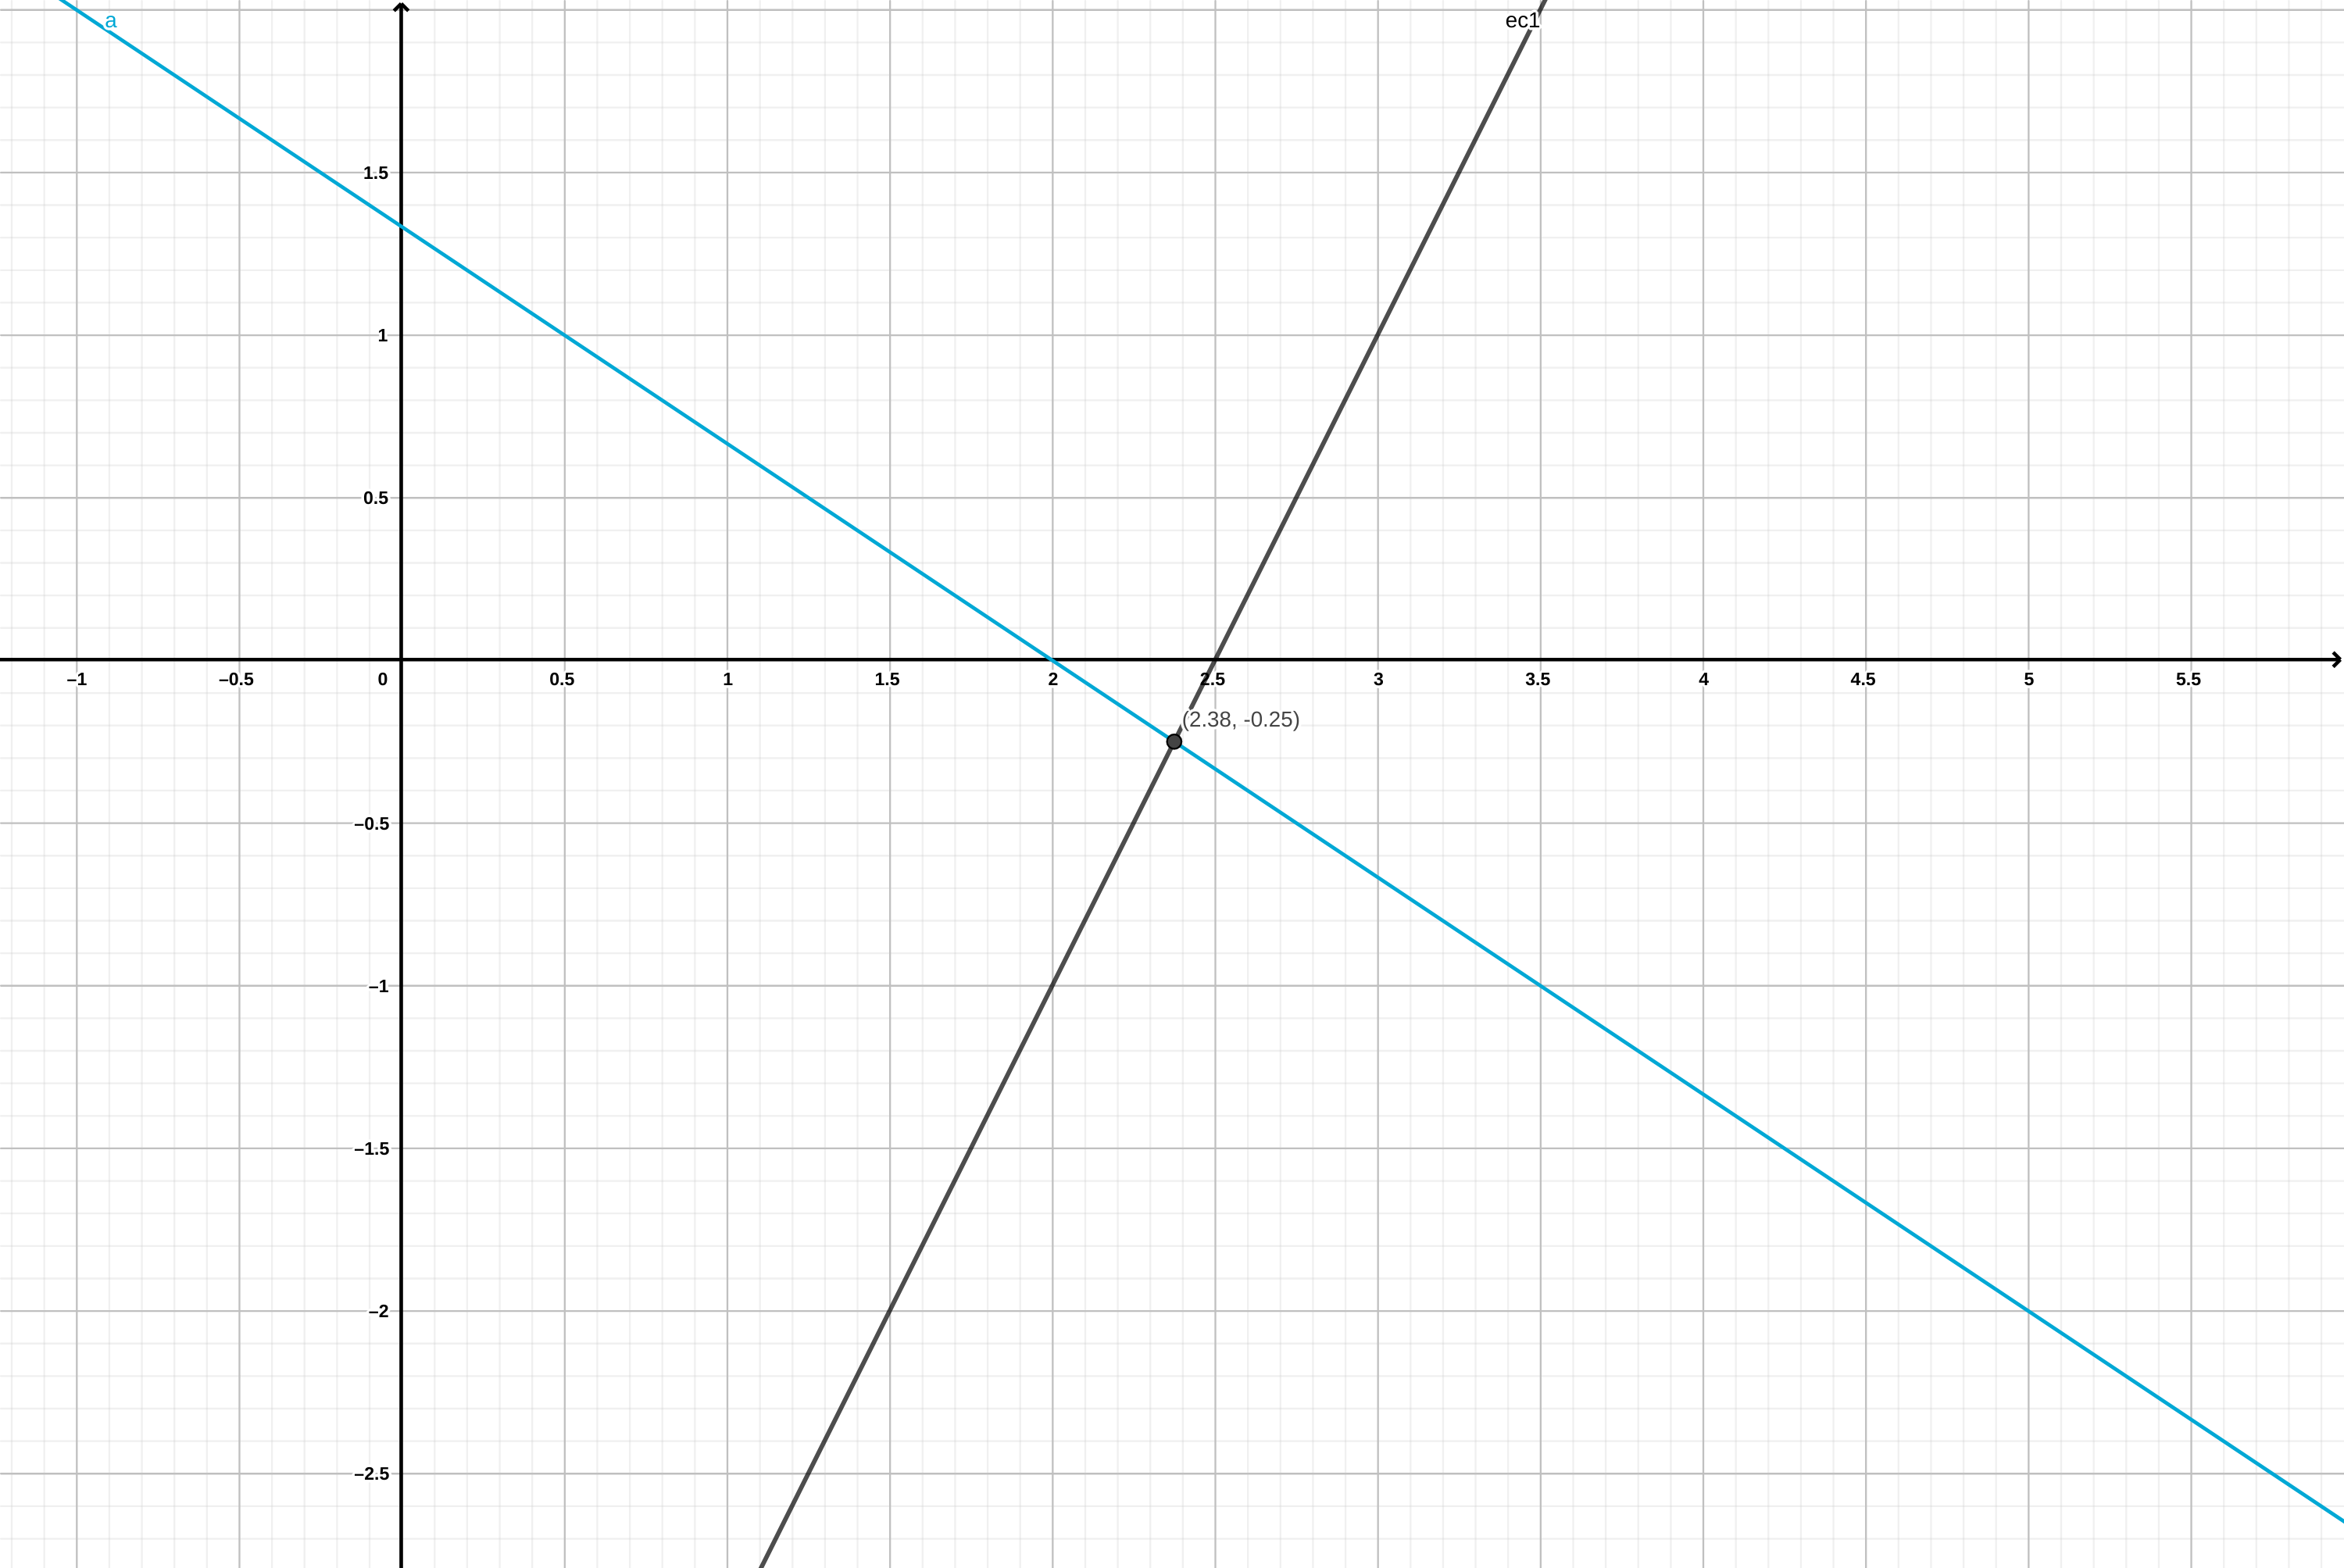
\includegraphics{Unidad-II/Soln-grafica-1} 

}

\caption{Solución gráfica del sistema de ecuaciones para dos variables}\label{fig:unnamed-chunk-23}
\end{figure}

\hypertarget{soluciuxf3n-algebruxe1ica}{%
\subsection{Solución algebráica}\label{soluciuxf3n-algebruxe1ica}}

El método más sencillo en esta ocasión sería resolver la ecuación 2 para \(y\), pues la podemos simplificar dividiendo ambos lados entre 2:

\[ (4x - 2y)/2 = (10)/2 \rightarrow 2x - y = 5\]
de donde obtenemos que:

\[y = 2x-5\]

Este valor de \(y\) en térmonos de \(x\), lo podemos sustituir en, la ecuación 1:

\[2x+3(2x-5) = 4\]

y resolvemos para \(x\) para obtener:

\[8x = 19 \rightarrow x = 19/8=2.375\]

Y entonces sustituimos a \(x\) en:

\(y = 2(2.375) - 5 = -0.25\)

Como se puede apreciar, resolver simples ecuaciones lineales puede ser laborioso. Es por ello que se desarrolló el álgebra de matrices, para resolver de eficientemente, sistemas de ecuaciones lineales con muchas variables. En esta unidad revisaremos brevemente los conceptos y técnicas más importantes del álgebra de matrices.

\hypertarget{sistemas-lineales-sin-soluciuxf3n}{%
\subsection{Sistemas lineales sin solución}\label{sistemas-lineales-sin-soluciuxf3n}}

En ocasiones, aunque un sistema de ecuaciones sea aparentemente completo, puede no tener solución. Por ejemplo el sistema:

\begin{align}
x + y & = 1 \\
2x + 2y & = 4
\end{align}

no tiene solución, lo cual se manifiesta gráficamente como dos líneas paralelas. Esto quiere decir que no existe un par de valores \(x\) y \(y\) que satisfagan las ecuaciones del sistema.

\begin{figure}

{\centering 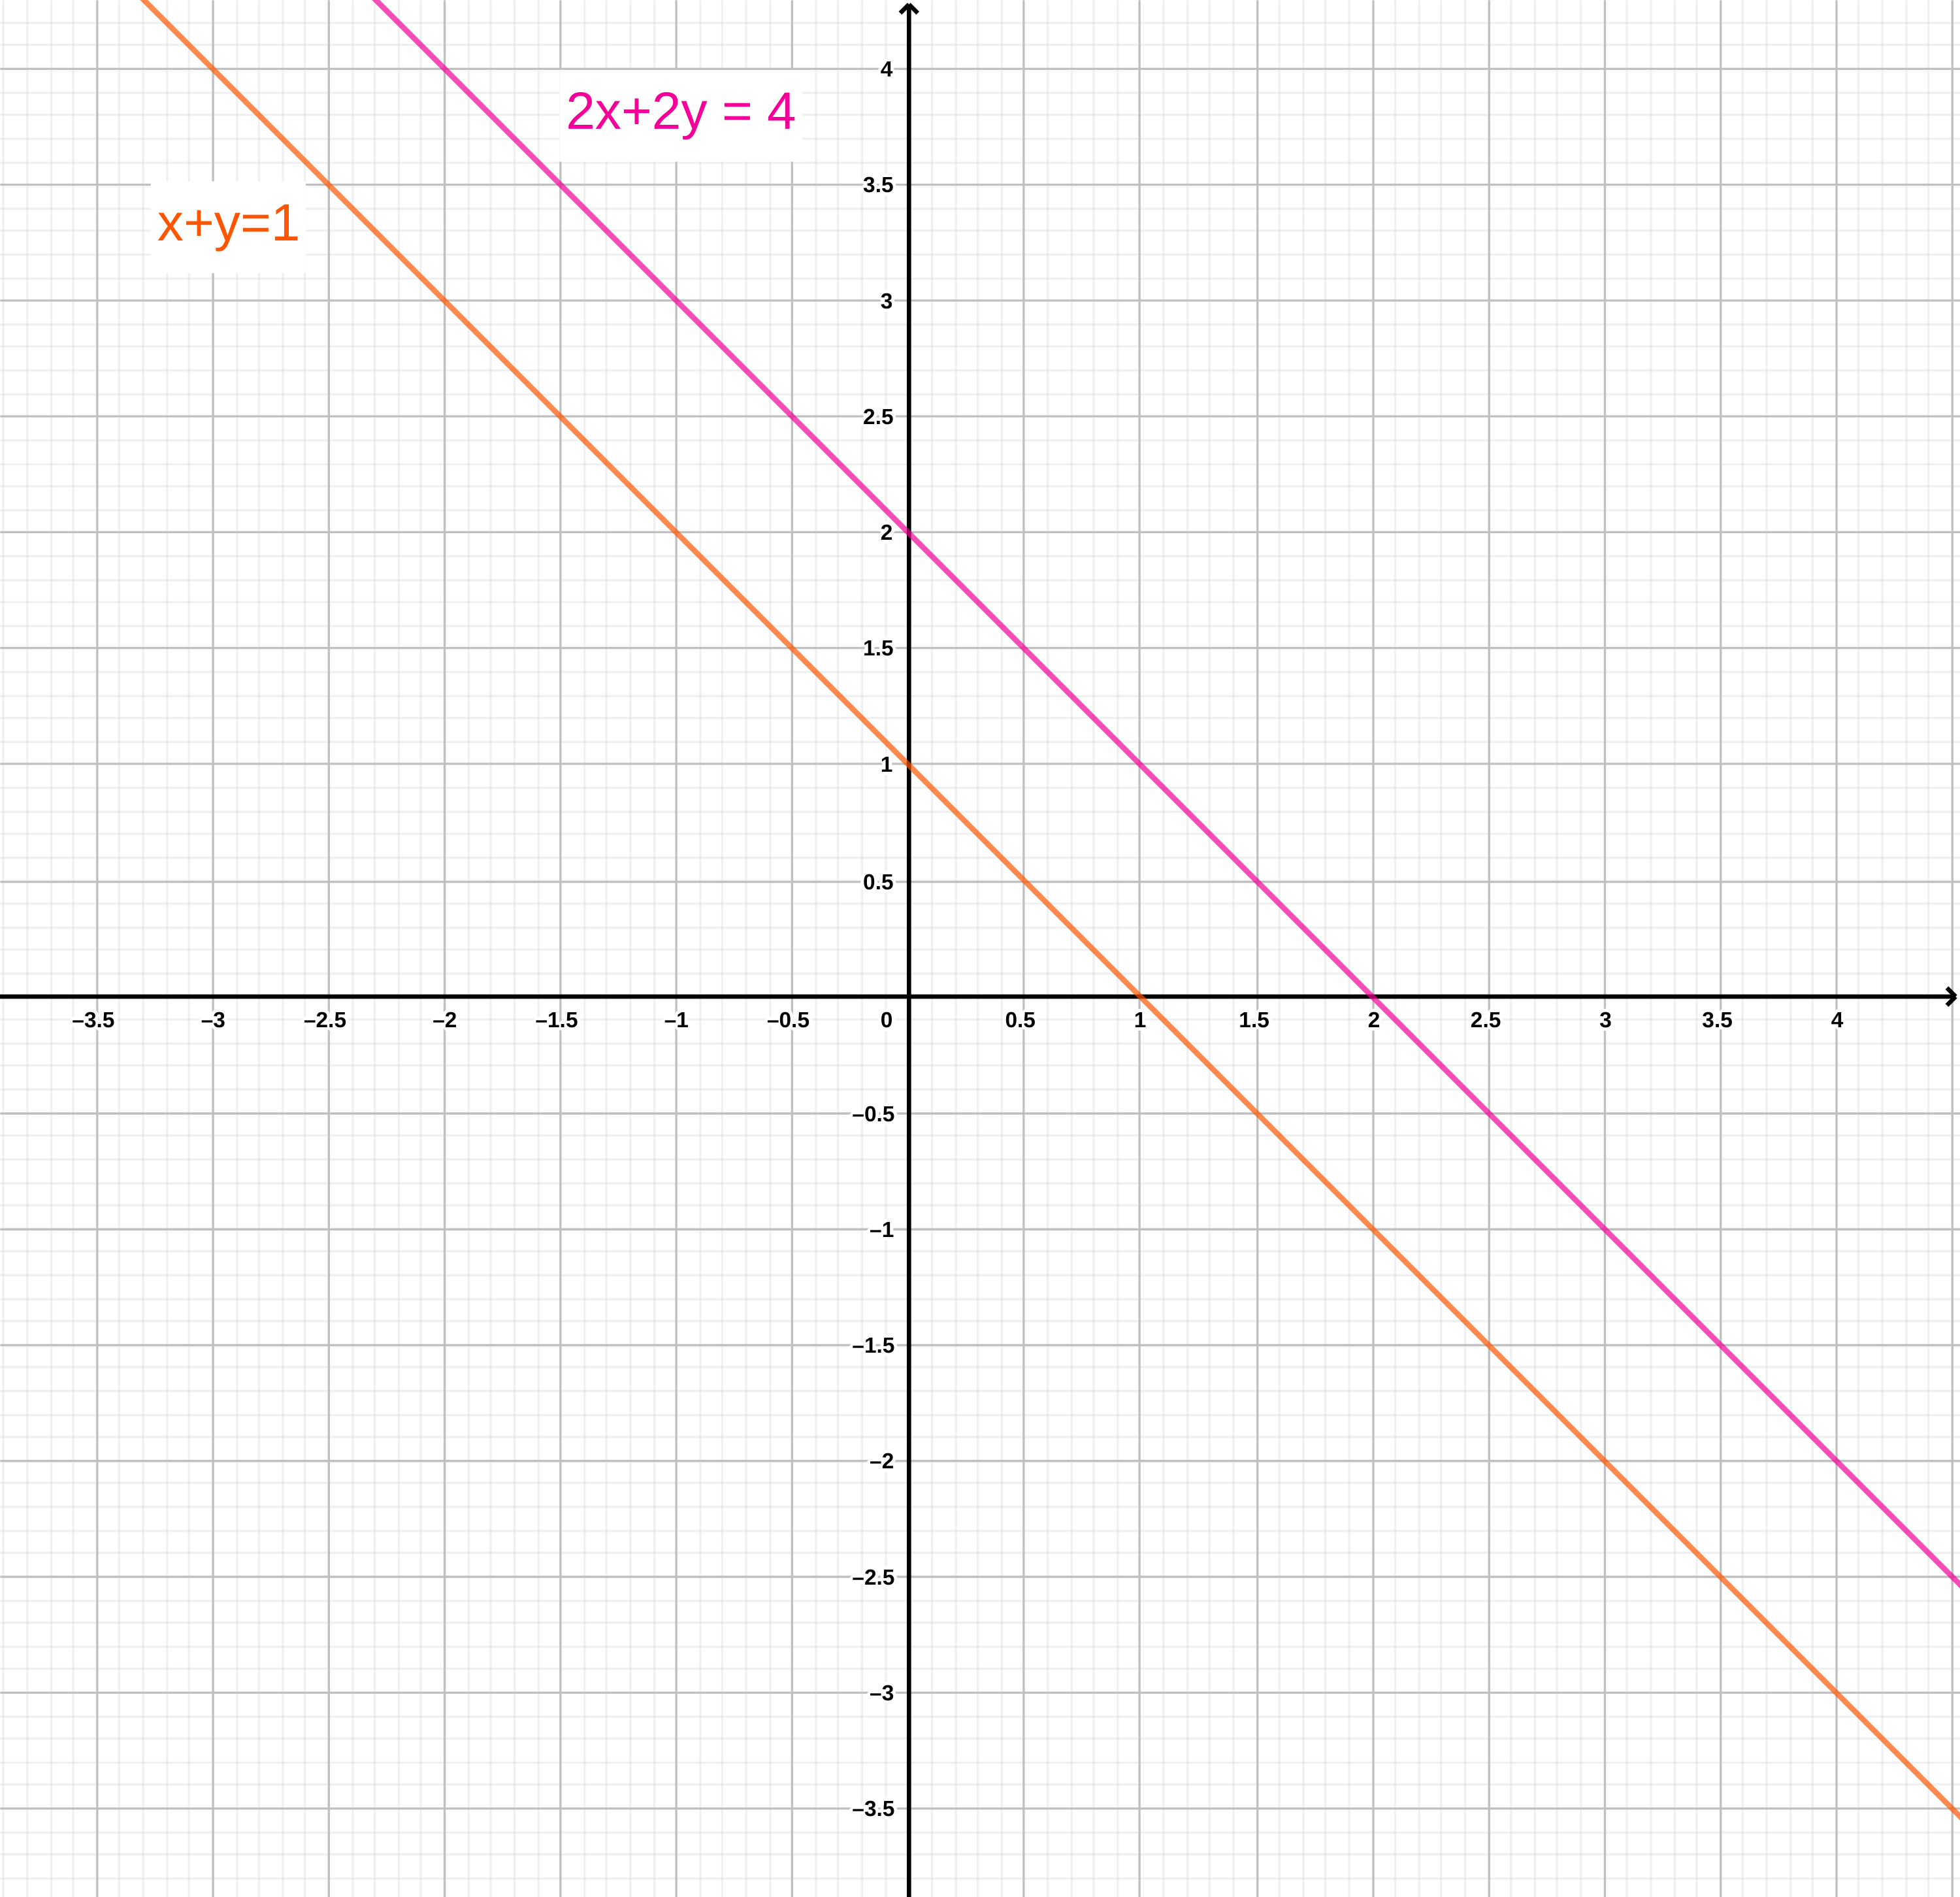
\includegraphics{Unidad-II/Sistema-no-solucion} 

}

\caption{Representación gráfica de un sistema linea sin solución.}\label{fig:sin-soln}
\end{figure}

Si intentamos sumar o restar ambas ecuaciones terminamos con una contradicción. Tomemos por ejemplo la primera ecuación, multiplicada por \(-2\) para obtener:

\[(x + y = 1) \times -2 \rightarrow -2x-2y = -2\]

Y al sumarla a la segunda ecuación:

\[2x - 2x + 2y - 2y = 4-2 \rightarrow 0 = 2\]

\hypertarget{resolviendo-sistemas-lineales-muxe1s-complejos}{%
\subsection{Resolviendo sistemas lineales más complejos}\label{resolviendo-sistemas-lineales-muxe1s-complejos}}

Cualquier sistema de ecuaciones lineales son solución se puede revolver con los métodos que hemos aprendido hasta el momento. Como hemos visto, en estos métodos es fácil cometer errores, máxime con sistemas más complejos con muchas variables y ecuaciones. El método ideal sería aquel que:

\begin{enumerate}
\def\labelenumi{\arabic{enumi}.}
\tightlist
\item
  Evita manipulaciones riesgosas de las ecuaciones
\item
  Permite encontrar todas las soluciones posibles
\item
  Permite identificar sistemas sin solución
\end{enumerate}

En la tarea de aprender a utilizar dichos métodos cabe resaltar que las incógnitas (\(x, y, z, \dots\)) juegan un papel secundario, lo más importante son los coeficientes de cada una en las distintas ecuaciones.

Para comenzar a visualizar un sistema lineal como matriz, echemos un vistazo al siguiente sistema:

\begin{align}
x+y+z+t & = 1 \\
x-y-z+t & = 3 \\
-x-y+z-t & = 1\\
-3x+y-3z-3t &= 4
\end{align}

cuyos coeficientes podemos representar en una matriz como:

\[A = \left[
\begin{array}{rrrr}
1 & 1 & 1 & 1 \\
1 &-1 &-1 & 1 \\
-1&-1 & 1 &-1 \\
-3& 1 &-3 &-3
\end{array}
\right]\]

Nota que cada columna corresponde con cada una de las variables \(x, y, z, t\), y los números que contiene la matriz \(A\) son sus coeficientes. Usando este mismo arreglo, podemos representar todo el sistema de ecuaciones como el producto de un vector \(x, y, z, t\) y la matriz \(A\):

\begin{equation}
\left[
\begin{array} {r}
x \\ y \\ z \\ t
\end{array}
\right]
\left[
\begin{array}{rrrr}
1 & 1 & 1 & 1 \\
1 &-1 &-1 & 1 \\
-1&-1 & 1 &-1 \\
-3& 1 &-3 &-3
\end{array} 
\right] = 
\left[\begin{array}{r}
1 \\ 3 \\ 1 \\ 4
\end{array}\right] \label{eq:sist-matriz}
\end{equation}

Dado que para las operaciones necesarias para resolverlo, sólo necesitamos la matriz de coeficientes \(A\) y el vector de equivalencias podemos representar el sistema con su matriz aumentada:

\begin{equation}
\left[
\begin{array}{rrrr|l}
1 & 1 & 1 & 1 & 1\\
1 &-1 &-1 & 1 & 3\\
-1&-1 & 1 &-1 & 1\\
-3& 1 &-3 &-3 & 4
\end{array} \right] \label{eq:Aumentada}
\end{equation}

Para resolver sistemas como este necesitamos aprender a hacer algunas operaciones con filas que no alteran el estado del sistema lineal:

\begin{enumerate}
\def\labelenumi{\arabic{enumi}.}
\tightlist
\item
  Intercambiar filas
\item
  Multiplicar una fila por un escalar \(c \neq 0\)
\item
  Sumar dos filas
\end{enumerate}

Ninguna de estas operaciones afectan las soluciones posibles del sistema (si las hay). Utilizando estas operaciones, la meta es transformar la matriz aumentada (\eqref{eq:Aumentada}), en un a matriz que contenga ceros bajo la diagonal (\textbf{Triángulo superior}), y así poder sustituir los valores comenzando con la última fila. El sistema de ecuaciones \eqref{eq:sist-matriz}, no tiene solución, por lo que solamente nos sirve, por el momento para establecer los conceptos. A continuación lo aplicamos con un sistema más sencillo.

\hypertarget{ejemplo}{%
\subsection{Ejemplo}\label{ejemplo}}

Dado el sitema linea:

\begin{align}
2x - 1y + 3z &= 9\\
3x + 5y - z  &= 10\\
4x + 2y - 3z &= -1
\end{align}

la matriz aumentada es:

\begin{equation}
\left[
\begin{array}{rrr|l}
 2 & -1& 3 & 9 \\
 3 & 5 &-1 & 10\\
 4 & 2 &-3 &-1
\end{array}
\right]
\begin{array}
\ (F_1) \\ (F_2) \\ (F_3)
\end{array}
\end{equation}

A continuación se muestra en el lado izquierdo, las operaciones correspondientes a las filas de las matrices:

\begin{equation}
\begin{array}{r}
(F_1) \\ -3(F_1)+2(F_2) \\ 2(F_1)-(F_3)
\end{array}
\left[
\begin{array}{rrr|r}
2 &-1 & 3 & 9 \\
0 &13 &-11&-7 \\
0 &-4 & 9 &19
\end{array}
\right]
\begin{array}{r}
\ (F_4) \\ (F_5) \\ (F_6)
\end{array}
\end{equation}

Ahora la fila 1 se llama \((F_4)\), hicimos \(-3(F_1)+2(F_2)\) para eliminar el coeficiente \(a_{2,1} = 3\), y ahora lo llamamos \((F_5)\). Lo único que debemos hacer ahora, es encontrar cómo eliminar \(a_{2,3}\) en \((F_6)\), para obtener la matriz con ceros bajo la diagonal:

\begin{equation}
\begin{array}{r}
(F_4) \\ (F_5) \\ 4(F_5)+13(F_6)
\end{array}
\left[
\begin{array}{rrr|r}
2 &-1 & 3 & 9 \\
0 &13 &-11&-7 \\
0 & 0 &73 &219
\end{array}
\right]
\begin{array}{r}
(F_7) \\ (F_8) \\ (F_9)
\end{array}
\end{equation}

A partir de aquí, tenemos una ecuación on una sola variable:

\[73z = 219\]
Con la cual podemos sustituir desde \((R_9)\) hacia \((R_7)\) para obtener los valores de \(x\) y \(y\) que satisfacen al sistema lineal.

\hypertarget{sistemas-indeterminados}{%
\subsection{Sistemas indeterminados}\label{sistemas-indeterminados}}

Cuando hay más variables que ecuaciones, no es posible encontrar una solución única al sistema, veamos un ejemplo de estos sistemas:

\begin{align}
2x+2y-z &= 1 \\
2x-y+z &= 2
\end{align}

cuya matriz aumentada es:

\begin{equation}
\left[
\begin{array}{rrr|r}
2 & 2 & -1& 1 \\
1 & -1& 1 & 2
\end{array} \right]
\begin{array}
(F_1) \\ (F_2)
\end{array}
\end{equation}

Lo primero que notamos es que, al haber más variables que ecuaciones, la matriz de coeficientes, tiene más columnas que filas. Entonces, vamos a comenzar por eliminar el coeficiente \(a_{2,1} = 2\), haciendo \((F_1)-F_2\):

\begin{equation}
\begin{array}{r}
(R_1) \\ (R_1) - (R_2)
\end{array}
\left[ 
\begin{array}{rrr|r}
2 & 2 &-1 & 1\\
0 & 3 &-2 &-1
\end{array}
\right]
\begin{array}{r}
(R_3) \\ (R_4)
\end{array}
\end{equation}

A partir de este punto sólo podemos expresar las soluciones para \(x\) y \(y\) en términos de \(z\):

\begin{align}
2x + 2y - z &= 1 \\
3y - 2z & = -1
\end{align}

Por lo tanto:

\[y = - \frac{1}{3} + \frac{2}{3}z\]

y sustituyendo \(y\) en la primera ecuación encontramos que:

\[x = \frac{5}{6} - \frac{1}{6}z\]

Para reportar un conjunto de soluciones para todo el sistema, podemos crear una variable ficticia \(t = z\), con lo que la solución al sistema es:

\[\left\{(x, y, z): x = \frac{5}{6} - \frac{1}{6}z, y = - \frac{1}{3} + \frac{2}{3}z, z = t \right\}\]

\hypertarget{operaciones-elementales-con-matrices}{%
\section{Operaciones elementales con matrices}\label{operaciones-elementales-con-matrices}}

Las operaciones elementales con matrices son similares a las aritméticas tradicionales. Para ejemplificarlas aquí denotamos a una matriz cualquiera con letras mayúsculas.

\hypertarget{suma-de-matrices}{%
\subsection{Suma de matrices}\label{suma-de-matrices}}

Si las matrices \(A\) y \(B\) tienenlas mismas dimensiones \(m \times n\) (\(m\) = número de filas, \(n\) = número de columnas):

\[A + B = C\]
La adición de \(A\) con \(B\) resulta en una tercera matriz \(C\) con dimensiones \(m \times n\), tanto si \(m = n\) como \(m \neq n\), es decir si las matrices \(A\) y \(B\) son cuadradas (\(m = n\)) como rectangulares.

Para esto tenemos que considerar qué sucede con los elementos de \(A\) y \(B\) dentro de \(C\):

\begin{equation}
A = \left[ 
\begin{array}{ccc}
a_{1, 2} & \dots & a_{1, n} \\
\vdots   & \ddots & \vdots \\
a_{n, 1} & \dots & a_{n, n}
\end{array} \right]
\end{equation}

\begin{equation}
B = \left[ 
\begin{array}{ccc}
b_{1, 2} & \dots & b_{1, n} \\
\vdots   & \ddots& \vdots \\
b_{n, 1} & \dots & b_{n, n}
\end{array} \right]
\end{equation}

\begin{equation}
C = \left[ 
\begin{array}{ccc}
a_{1, 2} + b_{1, 2} & \dots & a_{1, n} + b_{1, n} \\
\vdots   & \ddots & \vdots \\
a_{n, 1} + b_{n, 1} & \dots & a_{n, n} + b_{n, n}
\end{array} \right]
\end{equation}

Es claro que también:

\[B+A = C\]

Lo cual resulta importante resaltar pues la conmutatividad no funciona para la multiplicación de matrices. Otras cualidades de la adición de matrices, dadas las condiciones de dimensiones son:

\begin{enumerate}
\def\labelenumi{\arabic{enumi}.}
\tightlist
\item
  \((A+B)+C=A+(B+C)\)
\item
  \(A + 0 = A\)
\end{enumerate}

\hypertarget{multiplicaciuxf3n-por-un-escalar}{%
\subsection{Multiplicación por un escalar}\label{multiplicaciuxf3n-por-un-escalar}}

Es frecuente multiplicar una matriz por una constante \(c\), tal que \(c \times A = cA\):

\begin{equation}
c \times A = \left[ 
\begin{array}{ccc}
c  \cdot  a_{1, 2} & \dots & c \cdot a_{1, n} \\
\vdots   & \ddots & \vdots \\
c \cdot  a_{n, 1} & \dots & c  \cdot  a_{n, n}
\end{array} \right]
\end{equation}

\hypertarget{transposiciuxf3n}{%
\subsection{Transposición}\label{transposiciuxf3n}}

La transposición es el cambio de filas y columnas por columnas y filas, por ejemplo:

\begin{equation}
A = \left[ 
\begin{array}{rrr}
1 & 2 & 3 \\
4 & 5 & 6
\end{array}
\right]
\end{equation}

Con lo que la matriz \(A\) transpuesta \(A^T = A'\) es:

\begin{equation}
A' = \left[
\begin{array}{rr}
1 & 4 \\
2 & 5 \\
3 & 6
\end{array}
\right]
\end{equation}

\hypertarget{multiplicaciuxf3n-de-matrices}{%
\subsection{Multiplicación de matrices}\label{multiplicaciuxf3n-de-matrices}}

Para entender la multiplicación de matrices es necesario definirla, pues es más complicada que cualquiera de las operaciones que hemos visto anteriormente.

Supongamos que \(C\) es una matriz producto de la multiplicación de las matrices \(A\) y \(B\):

\[C = AB\]

Para que esto sea posible es necesario que \(A\) y \(B\) tengan dimensiones específicas pues:

\begin{equation}
C = \left[
\begin{array}{rrr}
 &        & \\
 & c_{ij} & \\
 &        &
\end{array}
\right] =
\left[ 
\begin{array}{ccc}
 & & & \\
a_{i, 1} & \dots & a_{i, l} \\
 & & &
\end{array}
\right] \times
\left[ 
\begin{array}{ccc}
 & b_{1, j} & \\
 & \vdots & \\
 & b_{l, j} & 
\end{array}
\right] \label{eq:mat-mult}
\end{equation}

Como resulta evidente, el número de \textbf{columnas} de la matriz \(A\) debe ser igual al número de \textbf{filas} de la matriz \(B\). De modo que podemos resumir que las dimensiones deben ser:

\begin{itemize}
\tightlist
\item
  \(A \rightarrow m \times l\)
\item
  \(B \rightarrow l \times n\)
\end{itemize}

\hypertarget{ejemplos}{%
\subsubsection{Ejemplos}\label{ejemplos}}

\begin{equation}
A = \left[ 
\begin{array}
\ 1 & 2 & 3 \\
-1& 0 & 4
\end{array}
\right]
\end{equation}

y

\begin{equation}
B = \left[ 
\begin{array}
\ 1 & 2 & 3 & -3\\
0 &-1 & 4 & 0 \\
-1& 0 &-2 & 1
\end{array}
\right]
\end{equation}

Solución:

\begin{equation}
C = AB = \left[ 
\begin{array}
\ 1 & 2 & 3 \\
-1& 0 & 4
\end{array}
\right]

\left[ 
\begin{array}
\ 1 & 2 & 3 & -3\\
0 &-1 & 4 & 0 \\
-1& 0 &-2 & 1
\end{array}
\right]
\end{equation}

Como vimos en la definición de multiplicación, tenemos que muiltiplicar las filas de \(A\) por las columnas de \(B\), para así obtener los elementos de \(C\). Hagamos entonces las operaciones elemento por elemento:

\begin{equation}
c_{1, 1} = \left[ 
\begin{array}{rrr}
\ 1 & 2 & 3
\end{array}
\right]
\left[\begin{array}
\ 1 \\ 0 \\ -1 \end{array}
\right] = (1)(1) + (2)(0) + (3)(-1)= -2
\end{equation}

\begin{equation}
c_{1, 2} = \left[
\begin{array}
1 & 2 & 3
\end{array}
\right]
\left[ 
\begin{array}
\ 2 \\ -1 \\0
\end{array}
\right] = (1)(2) + (2)(-1) + (3)(0) = 0
\end{equation}

Y así sucesivamente para obtener:

\begin{equation}
C = \left[ 
\begin{array}
\ c_{1, 1} & c_{1, 2} & c_{1, 3} & c_{1, 4} \\
c_{2, 1} & c_{2, 2} & c_{2, 3} & c_{2, 4} 
\end{array}
\right] =
\left[ 
\begin{array}
\ -2 & 0 & 5 & 0 \\
-5 & -2 & -11 & 7
\end{array}
\right]
\end{equation}

El resultado es una matriz con tantas filas como \(A\) y tantas columnas como \(B\). Es decir que si las dimensiones de \(A\) son \(m \times l\), y las de \(B\) son \(l \times n\), \(C\) tendrá dimensiones \(m \times n\).

\hypertarget{ejercicio-1}{%
\paragraph{Ejercicio}\label{ejercicio-1}}

Haz a mano los cálculos de \(c_{i, j}\) que nos faltaron para obtener los valores de \(C\).

\hypertarget{determinantes-y-matrices-inversas}{%
\section{Determinantes y matrices inversas}\label{determinantes-y-matrices-inversas}}

\hypertarget{matriz-identidad}{%
\subsection{Matriz identidad}\label{matriz-identidad}}

Antes de continuar, consideremos la posible existencia de una matriz \(I\) tal que \(A I = A\), es decir, una matriz que multiplicada por otra matriz de como resultado la matriz original. Esta matriz se conoce como la matriz identidad, y consiste de una matriz cuadrada con ceros en todas las posiciones excepto en la diagonal, por ejemplo:

\begin{equation}
I = \left[ 
\begin{array}{ccc}
\ 1 & 0 & 0 & 0 \\
  0 & 1 & 0 & 0 \\
  0 & 0 & 1 & 0 \\
  0 & 0 & 0 & 1 \\
\end{array}
\right]
\end{equation}

Por el contrario, una matriz inversa es quella matriz \(A^{-1}\), tal que \(AA^{-1} = I\), al multiplicarla por una matriz cualquiera \(A\) da como resultado la matriz identitaria.

\hypertarget{matriz-inversa}{%
\subsection{Matriz inversa}\label{matriz-inversa}}

La utilidad de este concepto se puede ejemplificar con un sistema de una sola ecuación:

\[2x = 10\]

Esta ecuación podemos concebirla como el producto de dos vectores con dimensiones \(1 \times 1\). Para resolverla es necesario multplicar ambos lados de la ecuación por el \textbf{inverso} del coeficiente de \(x\), de modo que:

\[2^{-1} \cdot 2x = 2^{-1} \cdot 10\]

\[x = \frac{1}{5}\]

Por lo tanto, si tenemos que para un sistema lineal la matriz \textbf{cuadrada} \(A\) de coeficientes puede ser invertida como \(A^{-1}\), esta última contiene la solución al sistema mismo:

\[XA = B\]

\[A^{-1}XA = A^{-1}B \rightarrow X = A^{-1}B\]

\hypertarget{definciuxf3n-de-matriz-inversa}{%
\subsubsection{Definción de matriz inversa}\label{definciuxf3n-de-matriz-inversa}}

Una matriz inversa de \(A\) es aquella matriz \(B\) que:

\[AB = BA = I_n\]

al ser multiplicada por \(A\) tiene como resultado la matriz identidad \(I_n\), con dimensiones \(n \times n\). La matriz inversa de \(A\) también recibe, como ya se mencionó el nombre \(A^{-1}\). Cuando se puede obtener la matriz \(A^{-1}\) de \(A\), se dice que esta última es \textbf{invertible} o \textbf{no-singular}, de lo contrario se le llama \textbf{singular}. Cabe resaltar que la matriz inversa \(A^{-1}\) es única para \(A\). Si llegaran a existir dos matrices inversas \(B\) y \(C\) de \(A\), entonces \(B=C\).

\hypertarget{obteniendo-una-matriz-inversa}{%
\subsubsection{Obteniendo una matriz inversa}\label{obteniendo-una-matriz-inversa}}

Para obtener una matriz inversa, también tenemos que resolver un sistema de ecuaciones lineales. Supongamos que \(A\) es una matriz de \(2 \times 2\):

\begin{equation}
A = \left[\begin{array}{ccc}
a_{1, 1} & a_{1, 2} \\
a_{2, 1} & a_{2, 2}
\end{array}
\right]
\end{equation}

Recordemos que \(A\) es la matriz de coeficientes para las variables \(x_1, x_2, \dots, x_n\). Entonces la matriz inversa de \(A\) es:

\begin{equation}
B = \left[\begin{array}{ccc}
b_{1, 1} & b_{1, 2} \\
b_{2, 1} & b_{2, 2}
\end{array}
\right]
\end{equation}

Por lo tanto la ecuación a resolver es:

\begin{equation}
\left[\begin{array}{ccc}
a_{1, 1} & a_{1, 2} \\
a_{2, 1} & a_{2, 2}
\end{array}
\right]
\left[\begin{array}{ccc}
b_{1, 1} & b_{1, 2} \\
b_{2, 1} & b_{2, 2}
\end{array}
\right] =
\left[\begin{array}{ccc}
1 & 0 \\
0 & 1
\end{array}
\right]
\end{equation}

donde las incógnitas son los elementos \(b_{1,1}, \dots b_{n,n}\) de \(B\), la matriz inversa.

\hypertarget{ejemplo-1}{%
\paragraph{Ejemplo}\label{ejemplo-1}}

Tenemos que encontrar la matriz inversa de la matriz de coeficientes:

\begin{equation}
A =
\left[\begin{array}{ccc}
2 & 5 \\
1 & 3
\end{array}
\right]
\end{equation}

Por lo tanto el sistema de ecuaciones a resolver es:

\begin{equation}
\left[\begin{array}{ccc}
2 & 5 \\
1 & 3
\end{array}
\right]
\left[\begin{array}{ccc}
b_{1, 1} & b_{1, 2} \\
b_{2, 1} & b_{2, 2}
\end{array}
\right] =
\left[\begin{array}{ccc}
1 & 0 \\
0 & 1
\end{array}
\right]
\end{equation}

Para ver las ecuaciones a resolver para \(B\), tenemos que multiplicar \(AB\), con lo que obtenemos:

\begin{align}
2 b_{1,1} + 5b_{2,1} = 1\ (F_1) & & 2b_{1, 2} + 5b_{2,2} = 0\ (F_1) \\ \notag
b_{1, 1} + 3b_{2,1} = 0\ (F_2) & & b_{1, 2} + 3b_{2, 2} = 1 (F_2 ) \notag
\end{align}

Utilizando los métodos que ya conocemos, podemos obtener las soluciones:

\begin{equation}
B = \left[ 
\begin{array}
\ b_{1, 1} & b_{1, 2} \\
b_{2, 1} & b_{2, 2}
\end{array}
\right] =
\left[ 
\begin{array}
\ 3 & -5 \\
-01 & 2
\end{array}
\right]
\end{equation}

\hypertarget{ejercicio-2}{%
\paragraph{Ejercicio}\label{ejercicio-2}}

Verifica que las soluciones para \(b_{1,1}, b_{1,2}, b_{2,1}, b_{2,2}\) sean las reportadas y que \(AB = I_2\)

\hypertarget{determinante-de-una-matriz}{%
\subsection{Determinante de una matriz}\label{determinante-de-una-matriz}}

Encontrar la matriz inversa de otra matriz \(A\) con dimensiones \(2 \times 2\), es más fácil de lo que parece, resolviendo el sistema \(AB = I_2\). Para cualquier matriz:

\begin{equation}
A = \left[
\begin{array}
\ a_{1,1} & a_{1,2} \\
a_{2,1} & a_{2,2}
\end{array}
\right]
\end{equation}

\(A\) es invertible si \(a_{1,1}a_{2,2} - a_{1,2}a_{2,1} \neq 0\) y si:

\begin{equation}
A^{-1} = 
  \frac{1}{a_{1,1}a_{2,2} - a_{1,2}a_{2,1}}
    \left[
      \begin{array}
        \ a_{2,2} & a_{1,2} \\
        a_{2,1} & a_{1,1}
      \end{array}
    \right] \label{eq:dos-dos}
\end{equation}

La expresión \(a_{1,1}a_{2,2} - a_{1,2}a_{2,1}\) para una matriz \(A\) de \(2 \times 2\) se conoce como el determinante y se denota como \(\mathrm{det} A\) ó \(|A|\).

Es posible calcular determinantes para cualquier matriz \(A\) con dimensiones \(n \times n\), y en todos los casos, es posible obtener \(A^{-1}\) si \(\mathrm{det}A \neq 0\). Las fórmulas para calcular el determinante de cualquier matriz se van complicando considerablemente conforme aumenta su tamaño, por lo que es necesario utilizar una calculadora de determinantes.

Aquí nos limitaremos a las fórmulas para determinantes de \(2\times 2\) (ecuación \eqref{eq:dos-dos}. La figura \ref{fig:det-3} muestra el procedimiento para una matrix de \(3 \times 3\).

\begin{figure}

{\centering 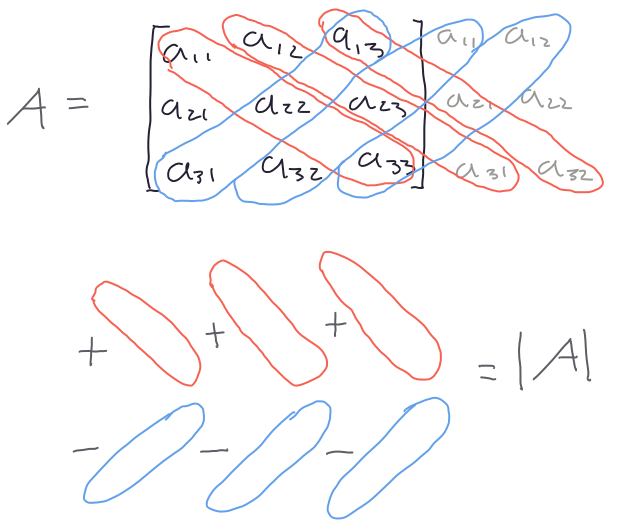
\includegraphics{Unidad-II/determ} 

}

\caption{Esquema del procedimiento para calcular el determinante de una matriz de 3 x 3.}\label{fig:det-3}
\end{figure}

\hypertarget{valores-y-vectores-propios}{%
\section{Valores y vectores propios}\label{valores-y-vectores-propios}}

Para hablar de vectores y valores propios necesitamos definir a un vector como una matriz con una sola columna y \(n\) filas. Todos los ejemplos que veremos aquí son de vectores de \(2 \times 1\).

Los vectores en el sentido en que los trataremos aquí, representan \emph{indicaciones} de movimiento en el plano cartesiano. Por ejemplo el vector:

\[\left[ 
\begin{array}{cc}
2 \\ 3
\end{array}
\right]\]

indica un movimiento de dos posiciones a la derecha en el eje \(x\) y tres posiciones arriba en el eje \(y\) (vector \(\mathbf{u}\) en la figura )

\begin{figure}

{\centering 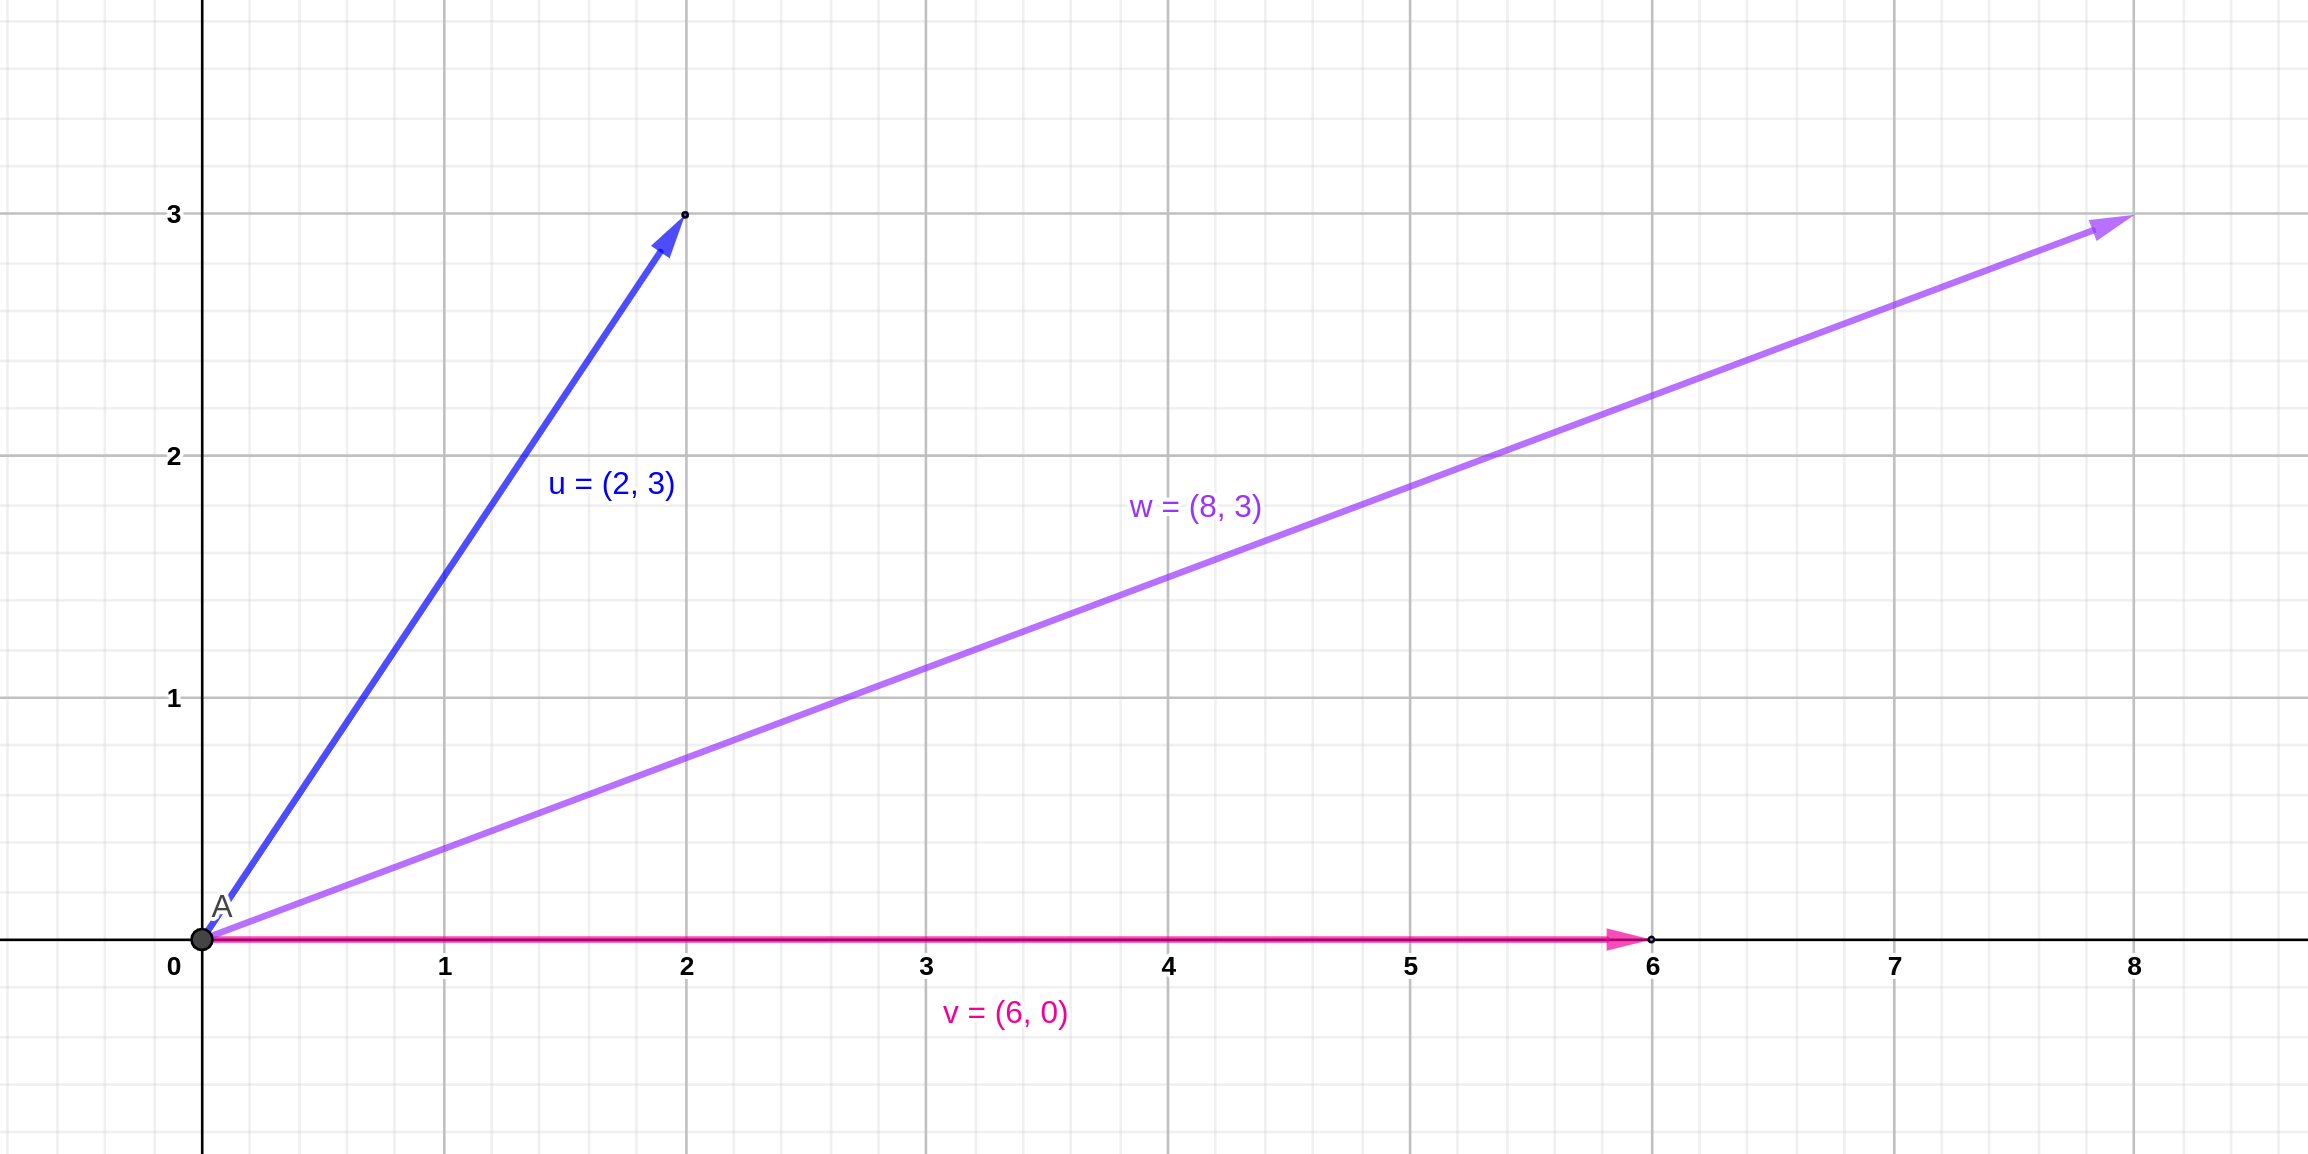
\includegraphics{Unidad-II/Vectores} 

}

\caption{Ejemplos de vectores **u** = (2, 3), **u**=(6, 0) y **w** = **u** + **v**.}\label{fig:vectores}
\end{figure}

Las operaciones con vectrores son iguales que las operaciones con matrices, de modo que el vector \(\mathbf{w}\) de la figura \ref{fig:vectores} es:

\[\mathbf{w} =\left[
\begin{array}{c}
2 \\ 3
\end{array}
\right]  + 
\left[
\begin{array}{c}
6 \\ 0
\end{array}
\right] = 
\left[
\begin{array}{c}
2 + 6 \\ 3 +0
\end{array}
\right] =
\left[
\begin{array}{c}
8 \\ 3
\end{array}
\right]\]

Cuando multiplicamos un vector cualquiera por un escalar, éste alargará el vector en relación a su magnitud, tal que :

\[
\mathbf{a} = 2 \times \mathbf{u} = \left[ \begin{array}{c} 4 \\ 6 \end{array} \right]
\]

\begin{figure}

{\centering 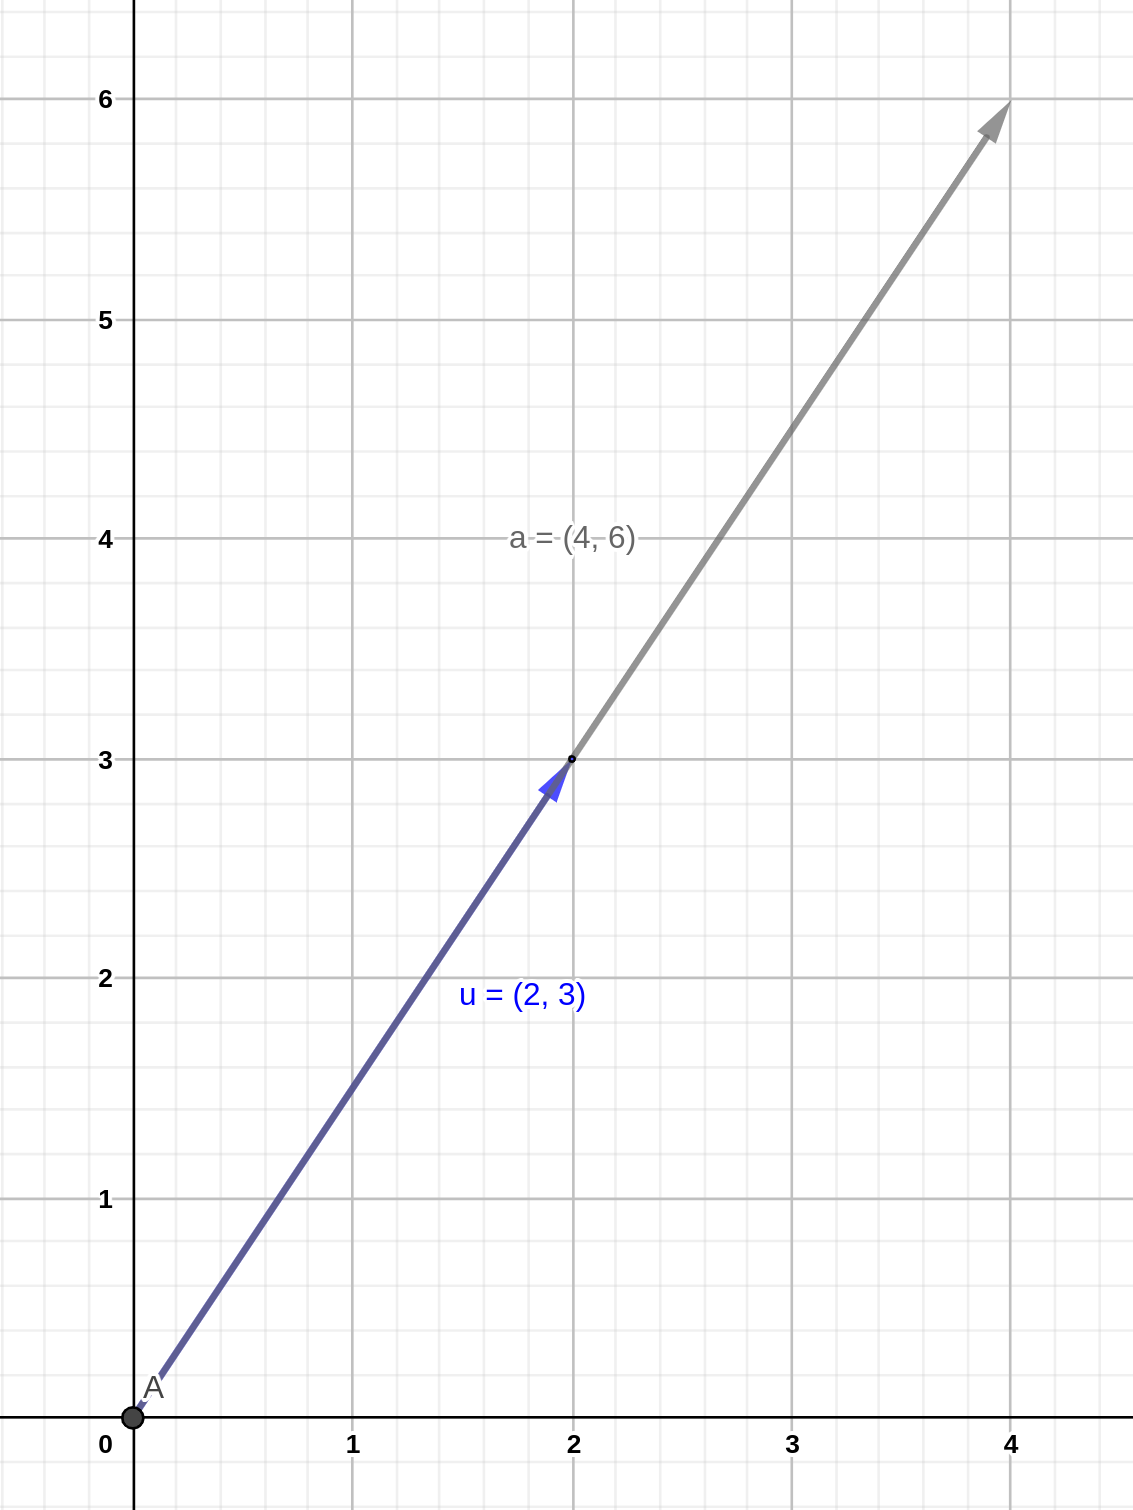
\includegraphics{Unidad-II/Mult-vector} 

}

\caption{Multiplicación de vector por un escalar.}\label{fig:vector-escalar}
\end{figure}

La operación que nos más concierne, sin embargo, en el caso de los valores y vectores propios es la multiplcación de un vector \(\mathbf{x}\) por una matriz \(A\).

Con base en las reglas de multiplicación sabemos que para el vector \(\mathbf{x}\) con dimensiones \(2 \times 1\) y la matriz \(A\) con dimensiones \(2 \times 2\), el producto \(A \mathbf{x}\) tendrá dimensiones de \(2 \times 1\). Dicha multiplicación se conoce como el mapa de \(\mathbf{x}\) y se escribe:

\begin{equation}
\mathbf{x} \mapsto A\mathbf{x} \label{eq:mapa}
\end{equation}

Por ejemplo:

\begin{equation}
    \left[ 
    \begin{array}{c}
    1 \\ 2
    \end{array}
    \right]
    \cdot
    \left[
    \begin{array}{cc}
    3 & 2 \\
    1 & 4
    \end{array}
    \right] = 
    \left[
    \begin{array}{c}
    7 \\ 9
    \end{array}
    \right]
\end{equation}

donde \(\mathbf{x}\) es el vector \((1, 2)\), y el mapa \(A \mathbf{x}\) es el vector \((7, 9)\).

El concepto de \textbf{vector y valor propio} está basado en \(\mathbf{x} \mapsto A \mathbf{x}\). Específicamente \(A \mathbf{x}\) es el vector propio y el valor propio es una constante que satisface:

\begin{equation}
A \mathbf{x} = \lambda \mathbf{x} \label{eq:valor-propio}
\end{equation}

Este tipo de operaciones tiene muchas aplicaciones, entre ellas está el resolver sistemas de ecuaciones. Aunque sólo veremos ejemplos con vectores de \(2 \times 1\), todos los ejemplos son generalizables a vectores con cualquier número de filas. El efecto de multiplicación de un vector propio \(\mathbf{x}\) por una matriz \(A\) es mostrado en la figura \ref{fig:vector-mat}. Todos los vectores fueron multiplicados por la misma matriz

\[A= \left[
\begin{array}{cc}
2 & 3 \\
0 & 1
\end{array}
\right]\]

\begin{figure}

{\centering 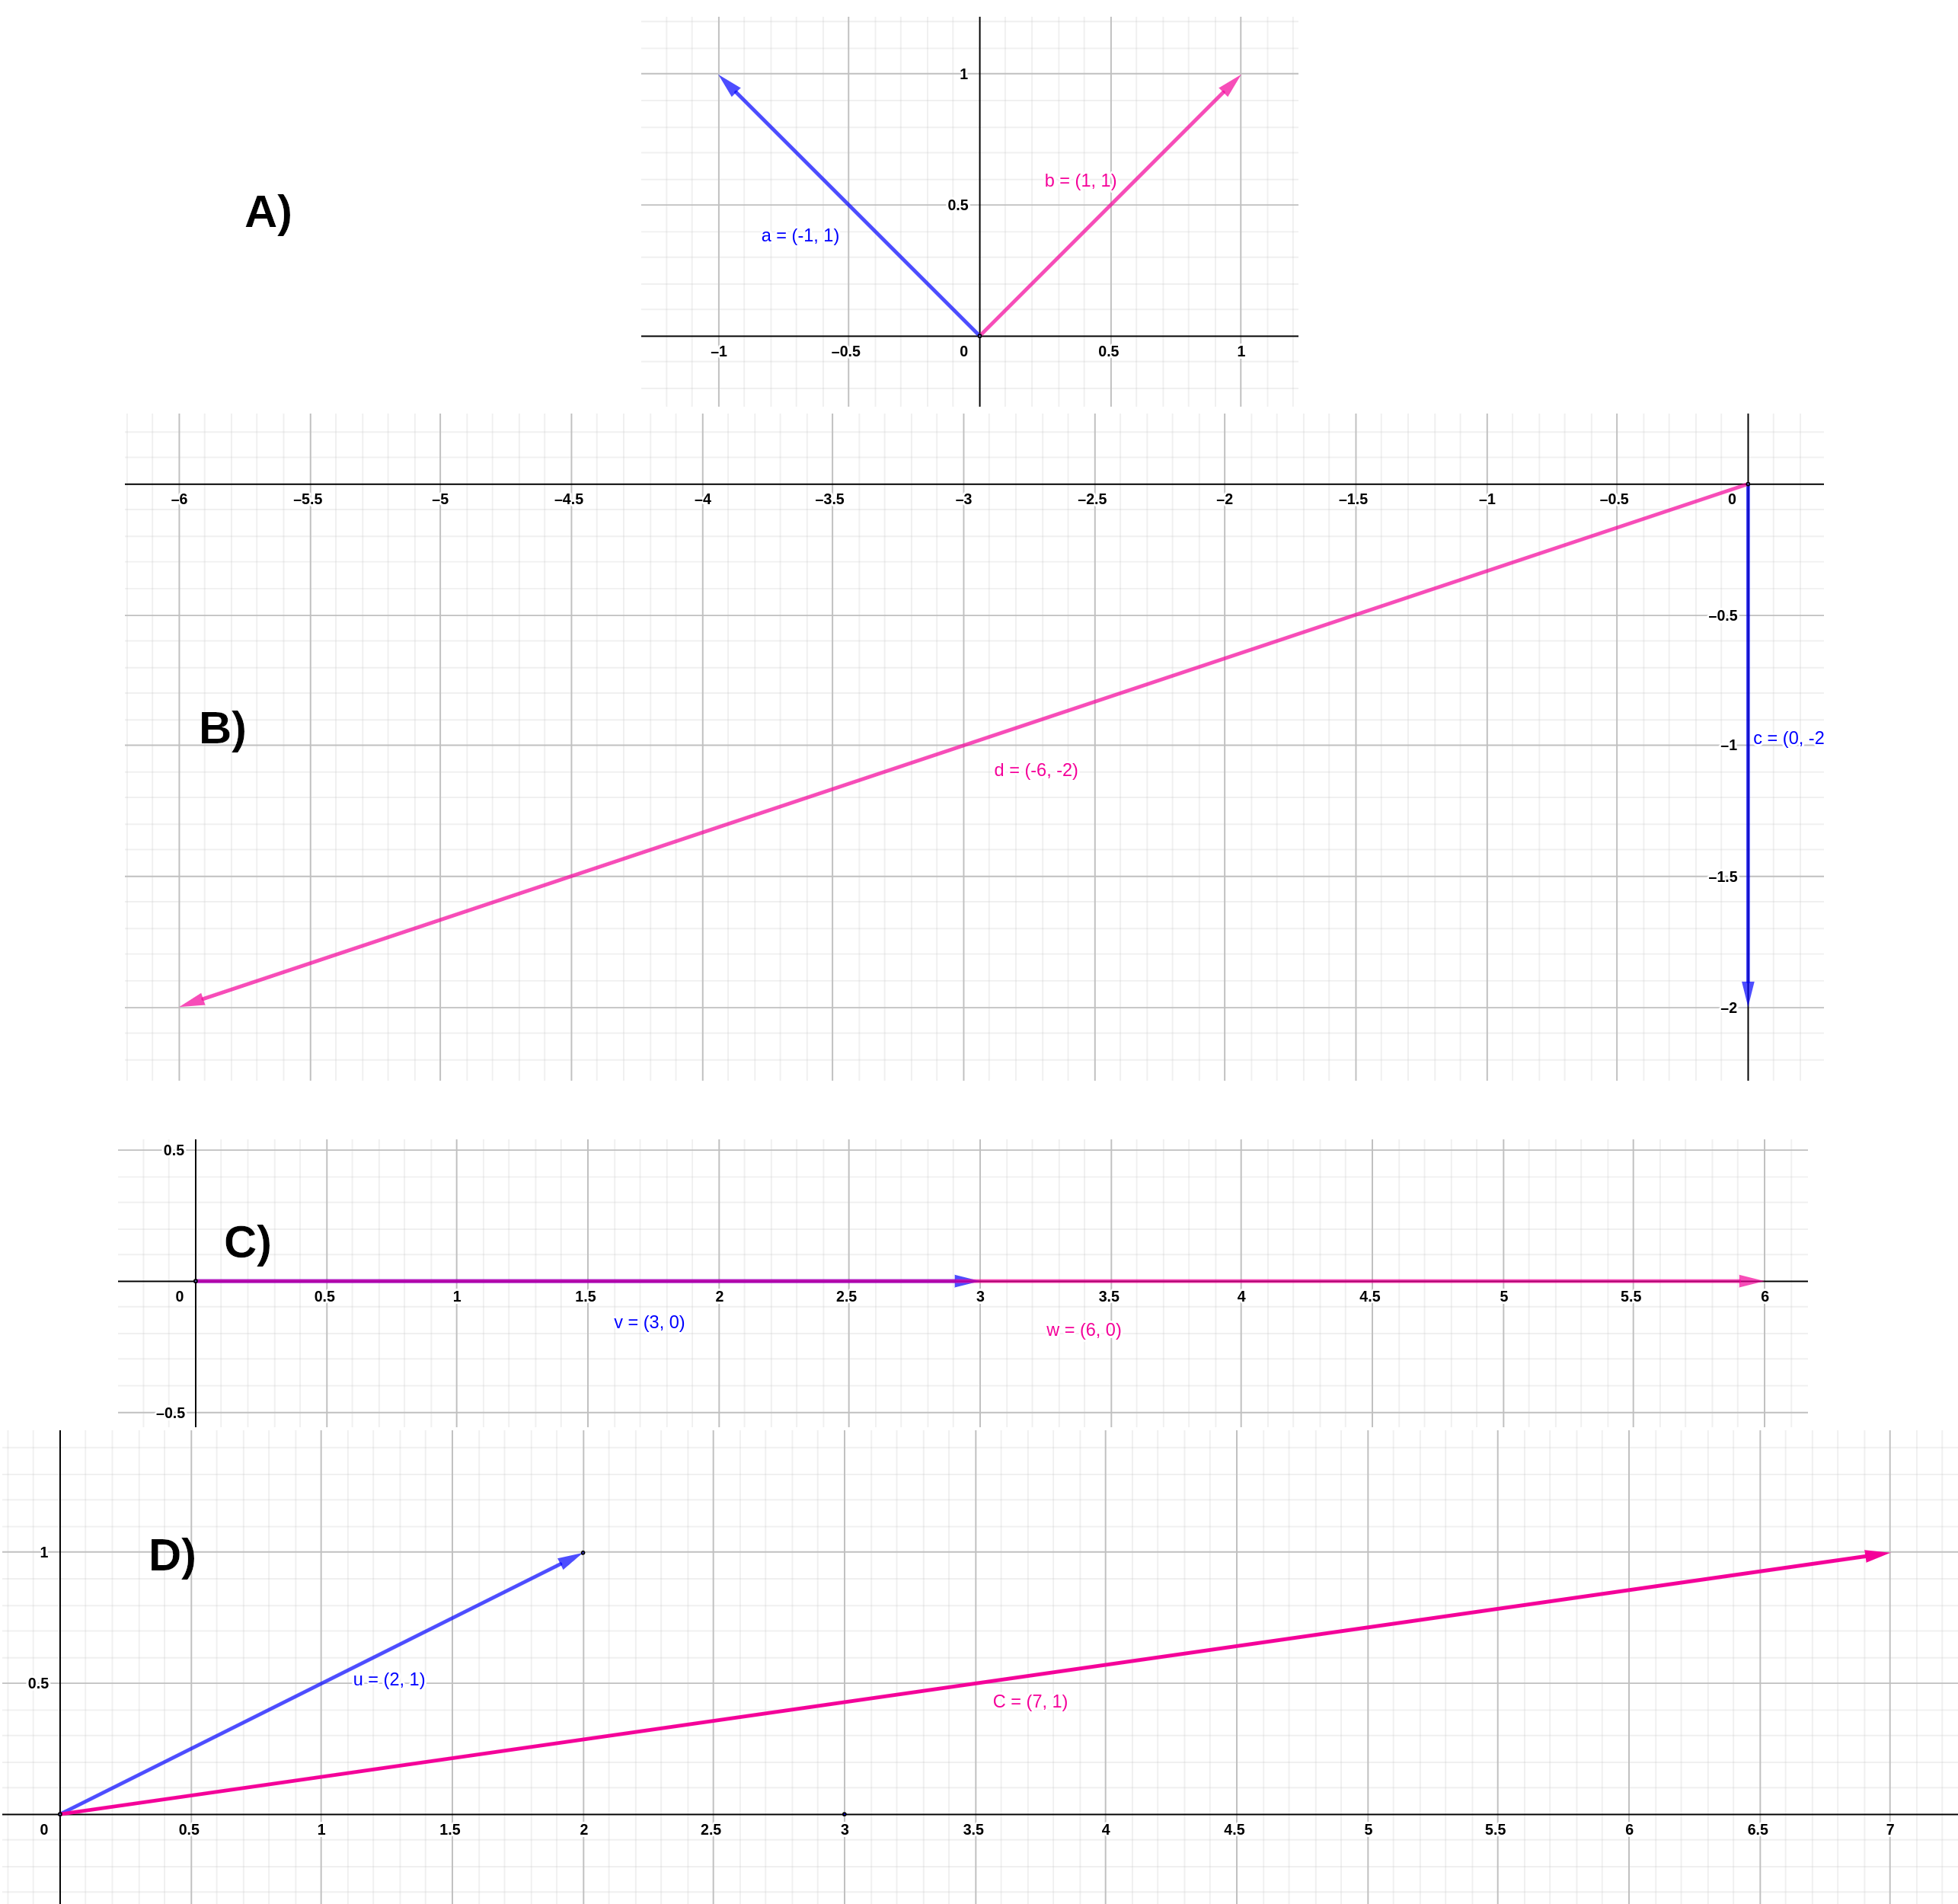
\includegraphics{Unidad-II/Eig-ejemplos} 

}

\caption{Ejemplos de multiplicación de un vector (azul) por una matriz y el resultante vector (rosa).}\label{fig:vector-mat}
\end{figure}

Como podemos ver, la multiplicación de \(\mathbf{x}\) por \(A\) tiene el efecto de rotar y cambiar la longitud del vector.

Existe una serie de técnicas para calcular \(\lambda\), y comenzaremos al igual que como hicimos para \(A^{-1}\), resolviendo la ecuación \eqref{eq:valor-propio}:

\[A \mathbf{x} = \lambda I \mathbf{x} \rightarrow (A - \lambda I) \mathbf{x} = 0\]
La parte \(\lambda I \mathbf{x}\) se debe a que \(I \mathbf{x} = \mathbf{x}\), pero necesitamos una matriz cuadrada para resolver a continuación.

Dado que \(\mathbf{x} \neq 0\), necesitamos que \(A - \lambda I\) sea singular (\(|A| = 0\)), de modo que necesitamos encontrar un valor de \(\lambda\) que satisfaga \(\det (A - \lambda I) = 0\). Entonces si nuestra matriz:

\[A = \left[
\begin{array}{cc}
1 & 2 \\
3 & 2
\end{array}
\right]\]

entonces:

\begin{equation}
A - \lambda I = \left[
\begin{array}{cc}
1 - \lambda & 2 \\
3 & 2 - \lambda
\end{array}
\right] \label{eq:A-problema}
\end{equation}

cuyo determinante será:

\[\begin{align}
(1 - \lambda)(2-\lambda) - (2)(3) &= 2 - 3 \lambda +\lambda^2 -6\\
& = \lambda^2 - 3 \lambda -4 \\
& = (\lambda + 1)(\lambda - 4)
\end{align}\]

por lo tanto tenemos las soluciones \(\lambda_1 = -1\) y \(\lambda_2 = 4\). Como es evidente, los vectores propios \(A \mathbf{x}\) que satisfacen los valores propios no son únicos, pero cada valor propio \(\lambda\) está asociado a un vector propio. Para los sistemas lineales con más de dos variables habrá tantos valores propios como dimensiones.

\hypertarget{vectores-propios}{%
\subsection{Vectores propios}\label{vectores-propios}}

Como se mostró arriba, el proceso del cálculo de los valores propios \(\lambda\) no requiere de conocer \(\vec{x}\), aunque mostramos una serie de ejemplos para vectores específicos. Entonces, debido a que \(\lambda\) es un atributo de la matriz de coeficientes \(A\), se puede generalizar el vector \(\vec{x}\) para encontrar todos los valores que contiene y que satisfacen \(A \vec{x} = \lambda \vec{x}\).

Utilizando la matriz \eqref{eq:A-problema}, tenemos que para \(\lambda_1 = -1\):

\begin{equation}
\left[
\begin{array}{cc}
1 & 2 \\
3 & 2
\end{array} 
\right]
\left[
\begin{array}{cc}
x_1  \\
x_2
\end{array} 
\right]
=
\left[
-1 \begin{array}{cc}
x_1  \\
x_2
\end{array}
\right]
\end{equation}

lo que se traduce en las siguiente ecuaciones

\begin{align}
x_1 + 2x_2 &= -x_1 \\ \notag
3x_1 + 2x_2 &= -x_2 \notag
\end{align}

y al resolverlas, encontramos las soluciones:

\begin{equation}
\left[ 
\begin{array}{c}
x_1 \\ x_2
\end{array}
\right] =
\left[ 
\begin{array}{c}
1 \\ -1
\end{array}
\right] 
\end{equation}

Sustituyendo \(\lambda_2 = 4\), obtenemos el vector propio \(\left[ \begin{array}{c} 2 \\ 3 \end{array} \right]\).

\hypertarget{unidad-iii-introducciuxf3n-al-cuxe1lculo-diferencial-e-integral}{%
\chapter{Unidad III: Introducción al cálculo diferencial e integral}\label{unidad-iii-introducciuxf3n-al-cuxe1lculo-diferencial-e-integral}}

\hypertarget{sucesiones}{%
\section{Sucesiones}\label{sucesiones}}

En matemáticas, de manera muy general, las sucesiones pueden ser entendidas como una función cuyo dominio \textbf{siempre} es el conjunto o un subconjunto de los números naturales, mientras que el codominio puede pertenecer a cualquier otro conjunto. En notación tradicional de funciones tenemos entonces que \(x \in \mathbb{N}\), mientras que:

\begin{equation}
y(x) \in \begin{cases}\mathbb{R}\\ \mathbb{Z}\\ \mathbb{N} \end{cases}
\end{equation}

La mayoría de las sucesiones, sin embargo que se utilizan en ecología, corresponden a:

\begin{equation}
    f: 
    \begin{aligned}[t] 
            \mathbb{N}_0 \rightarrow \mathbb{R} \\
            n \rightarrow f(n)
    \end{aligned}
\end{equation}

una función \(f\) de los números naturales, incluido el cero (\(\mathbb{N}_0\)) que produce números reales (\(\mathbb{R}\)), cuyo dominio es \(n\), y codominio es \(f(n)\).

Otra característica de las sucesiones es que sus elementos están ordenados, es decir, cada elemento en el dominio y codominio tiene un sitio particular, de modo que si los conjuntos \(a_n = \{A, B, C\}\) y \(a_m = \{C, A, B\}\), \(a_n \neq a_m\), puesto que, aunque contengan los mismos elementos \(A, B\) y \(C\), estos tienen posiciones diferentes dentro de \(a_n\) y \(a_m\).

\hypertarget{notaciuxf3n-de-sucesiones}{%
\subsection{Notación de sucesiones}\label{notaciuxf3n-de-sucesiones}}

Una sucesión de los números naturales suele nombrarse como \(\{a_n\}\), seguida de la regla de correspondencia entre el conjunto \(n\) y \(a\). Así por ejemplo:

\begin{equation} 
    \{a_n\} = 2n \label{eq:a2n}
\end{equation}

es una sucesión de los números naturales pares, tal que:

\[a_1 = 1, a_2 = 4, a_3 = 6, a_4 = 8 \dots\]
Esta notación, sin embargo no es universal, por ejemplo:

-\((a_n) = a_1, a_2, a_3, \dots\)

-\((a_k)_{k=1}^m = a_1, a_2, a_3, \dots, a_m\)

-\(\{a_n\}_{n \in \mathbb{N}} = a_1, a_2, a_3, \dots\)

\hypertarget{tipos-de-sucesiones}{%
\subsection{Tipos de sucesiones}\label{tipos-de-sucesiones}}

La sucesión anterior es un ejemplo muy sencillo y poco útil en la modelación ecológica, pero es un punto de partida para entender la notación y el concepto. Existen sucesiones, sin embargo, que tienen implicaciones importantes para el desarrollo de modelos dinámicos, como las \textbf{sucesiones por recurrencia}.

\hypertarget{sucesiones-recurrentes}{%
\subsubsection{Sucesiones recurrentes}\label{sucesiones-recurrentes}}

En estas sucesiones, la regla de correspondencia indica algún tipo de operación con elementos de \(n\) en posiciones previas. Así por ejemplo, la sucesión:

\begin{equation}
\{a_n\} = a_{n-1} + a_{n-2} \label{eq:fibonacci}
\end{equation}

se conoce como sucesión de Fibonacci, en la que, el elemento \(n\) se obtiene sumando los elementos \(n-1\) y \(n-2\) de la secuencia \(\{a_n\}\).

\begin{table}

\caption{\label{tab:fibo-tabla}Secuencia de Fibonacci para los diez primeros números naturales.}
\centering
\begin{tabular}[t]{r|r}
\hline
n & a\\
\hline
1 & 1\\
\hline
2 & 1\\
\hline
3 & 2\\
\hline
4 & 3\\
\hline
5 & 5\\
\hline
6 & 8\\
\hline
7 & 13\\
\hline
8 & 21\\
\hline
9 & 34\\
\hline
10 & 55\\
\hline
\end{tabular}
\end{table}

La secuencia de finonacci, tiene un comportamiento parecido a la función exponencial, en el sentido de que el crecimiento de \(a\) es más rápido conforme los valores de \(a\) son mayores.

\begin{figure}

{\centering 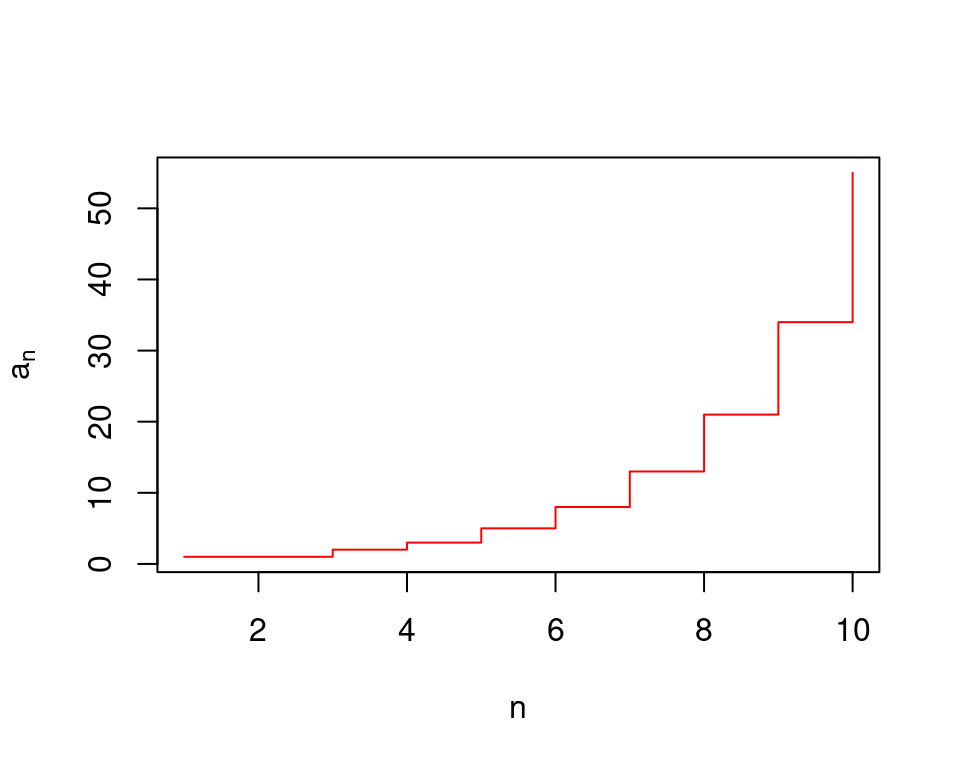
\includegraphics{Model-mate_files/figure-latex/fibo-fig-1} 

}

\caption{Representación gráfica de la secuencia de Fibonacci.}\label{fig:fibo-fig}
\end{figure}

\hypertarget{sucesiones-recurrentes-muxe1s-avanzadas}{%
\subsubsection{Sucesiones recurrentes más avanzadas}\label{sucesiones-recurrentes-muxe1s-avanzadas}}

Las sucesiones recurrentes pueden ser también concebidas como modelos dinámicos en tiempo discreto, donde el tiempo está representado por el conjunto de los números naturales, así, por ejemplo, el crecimiento de una población lo podemos representar como:

\begin{equation}
    N_{t} = r N_{t-1} \label{eq:susc-crec}
\end{equation}

Como podemos ver, en \eqref{eq:susc-crec}, el crecimiento por unidad de tiempo es lineal con respecto del número de individuos en el periodo de tiempo inmediatamente previo (\(rN_{t-1}\)).

\begin{figure}

{\centering 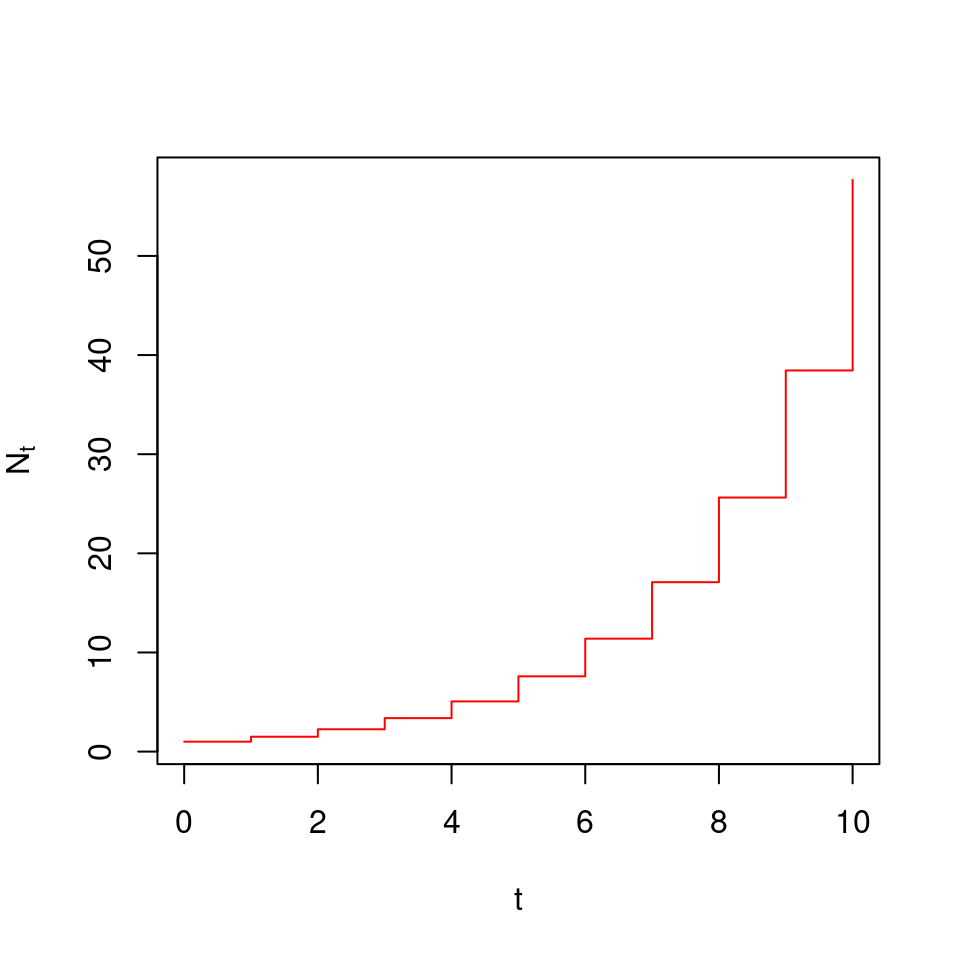
\includegraphics{Model-mate_files/figure-latex/susc-crec-1} 

}

\caption{Simulación de la sucesión de crecimiento poblacional en tiempo discreto, para 10 unidades de tiempo, con r = 1.5, y una población inicial de N = 1.}\label{fig:susc-crec}
\end{figure}

La sucesión descrita por la ecuación \eqref{eq:susc-crec} es fácil de simular con una computadora, con aplicaciones tan populares como las hojas de cáculo como excel.

Con este tipo de sucesiones, es posible comenzar a utilizar conceptos básicos de cálculo. Podemos por ejemplo, tomar la misma sucesión de la ecuación \eqref{eq:susc-crec}, con una población inicial de \(N = 50\), y \(r = 0.6\), y simular por un periodo de tiempo de 20, para ver hacia qué valor se aproxima \(N_t\) (\ref{fig:susc-decrec}).

\begin{figure}

{\centering 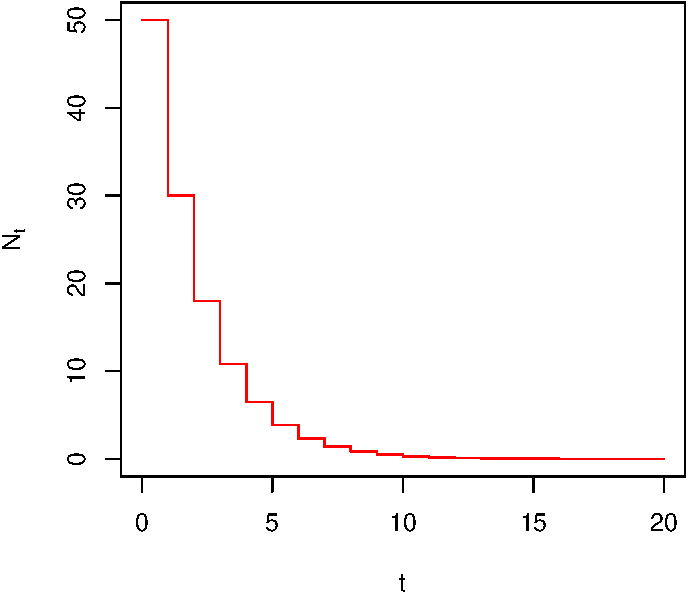
\includegraphics{Model-mate_files/figure-latex/susc-decrec-1} 

}

\caption{Simulación para un valor inicial de N = 50, por 20 unidades de tiempo, y r = 0.6}\label{fig:susc-decrec}
\end{figure}

En cada simulación, \(N_t\) cambia de acuerdo con el valor de \(N_{t-1}\). Como es evidente, si \(r > 1\), \(N_t\) crece, y mientras \(t \rightarrow \infty\), \(N_t \rightarrow \infty\). En el caso contrario, cuando \(r < 1\) y \(t \rightarrow \infty\), \(N_t \rightarrow 0\)

En estos casos, decimos que por ejemplo para \(r < 1\), \(N\) está acotada por \(0\). Hay otras sucesiones, por ejemplo la de crecimiento logístico, que está acotada por la capacidad de carga, incluso si \(r > 0\).

\begin{figure}

{\centering 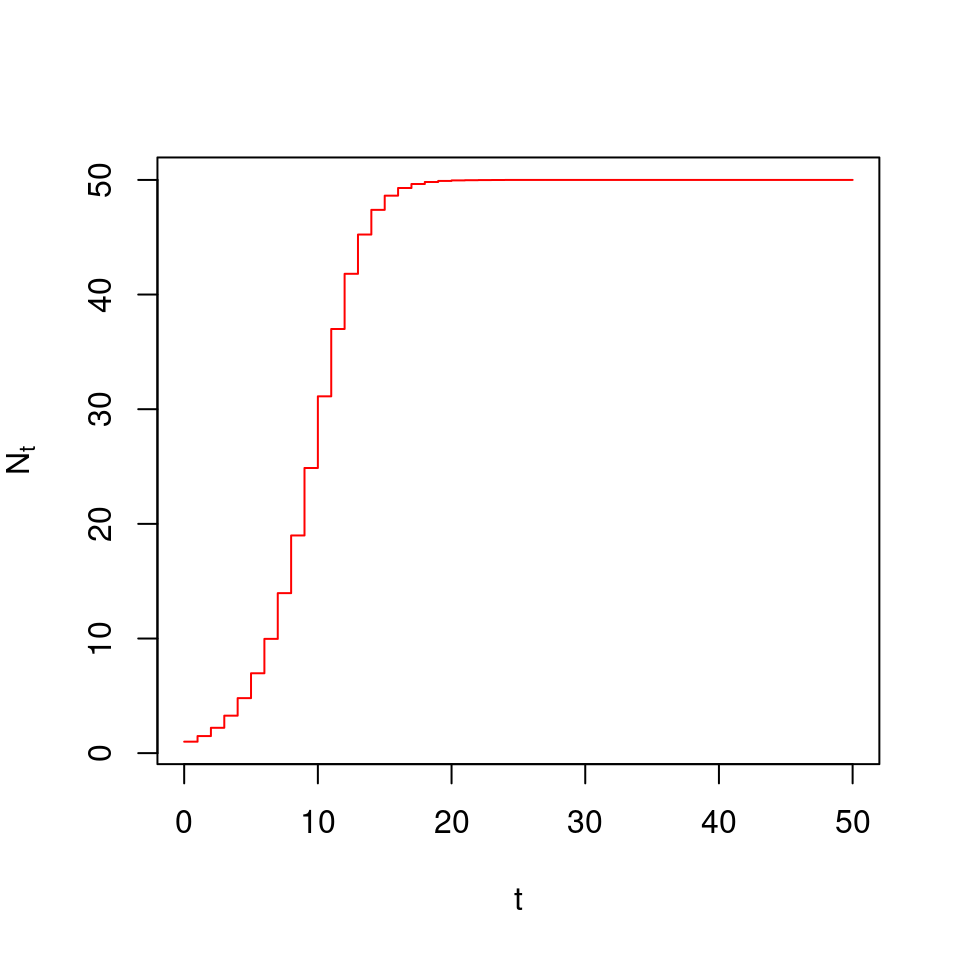
\includegraphics{Model-mate_files/figure-latex/susc-logis-1} 

}

\caption{Simulación para un valor inicial de N = 1, por 50 unidades de tiempo, r = 0.5, y capacidad de carga K = 50}\label{fig:susc-logis}
\end{figure}

La sucesión para el crecimiento logístico en tiempo discreto es:

\begin{equation}
N_{t} = N_{t-1} + r N_{t-1} \left(1 - \frac{N_{t-1}}{K} \right) \label{eq:susc-logis}
\end{equation}

\hypertarget{ejercicio-3}{%
\subsubsection{Ejercicio}\label{ejercicio-3}}

Utilizando la hoja de cálculo para la sucesión de crecimiento poblacional en tiempo discreto, adaptala para simular el crecimiento poblacional probando los valores de \(r\) dese 0.5 hasta 3.5 en incrementos de 0.25, y grafícalos. ¿Qué pasa con \(N_t\) con los valores de \(r\) probados?

\hypertarget{continuidad-y-luxedmites}{%
\section{Continuidad y límites}\label{continuidad-y-luxedmites}}

La continuidad y los límites son la puerta de entrada a la derivación y por lo tanto a las ecuaciones diferenciales. Cuando decimos que una función es contínua en un intervalo definido del dominio \((x_1, x_2)\), quiere decir que \(f(x)\) está definida para todos y cada uno de los posibles valores de \(x\) en ese intervalo. Existen muchas funciones que no son contínuas, por ejemplo:

\begin{equation}
    f(x) = \frac{x - 1}{x - 1} \label{eq:disc-1}
\end{equation}

Como es evidente, dicha ecuación está definida para todos los valores posibles de \(x\), excepto \(x = 1\), porque \(f(1) = \frac{1 - 1}{1-1} = \frac{0}{0}\), lo cual es una indeterminación, no existe.

\begin{figure}

{\centering 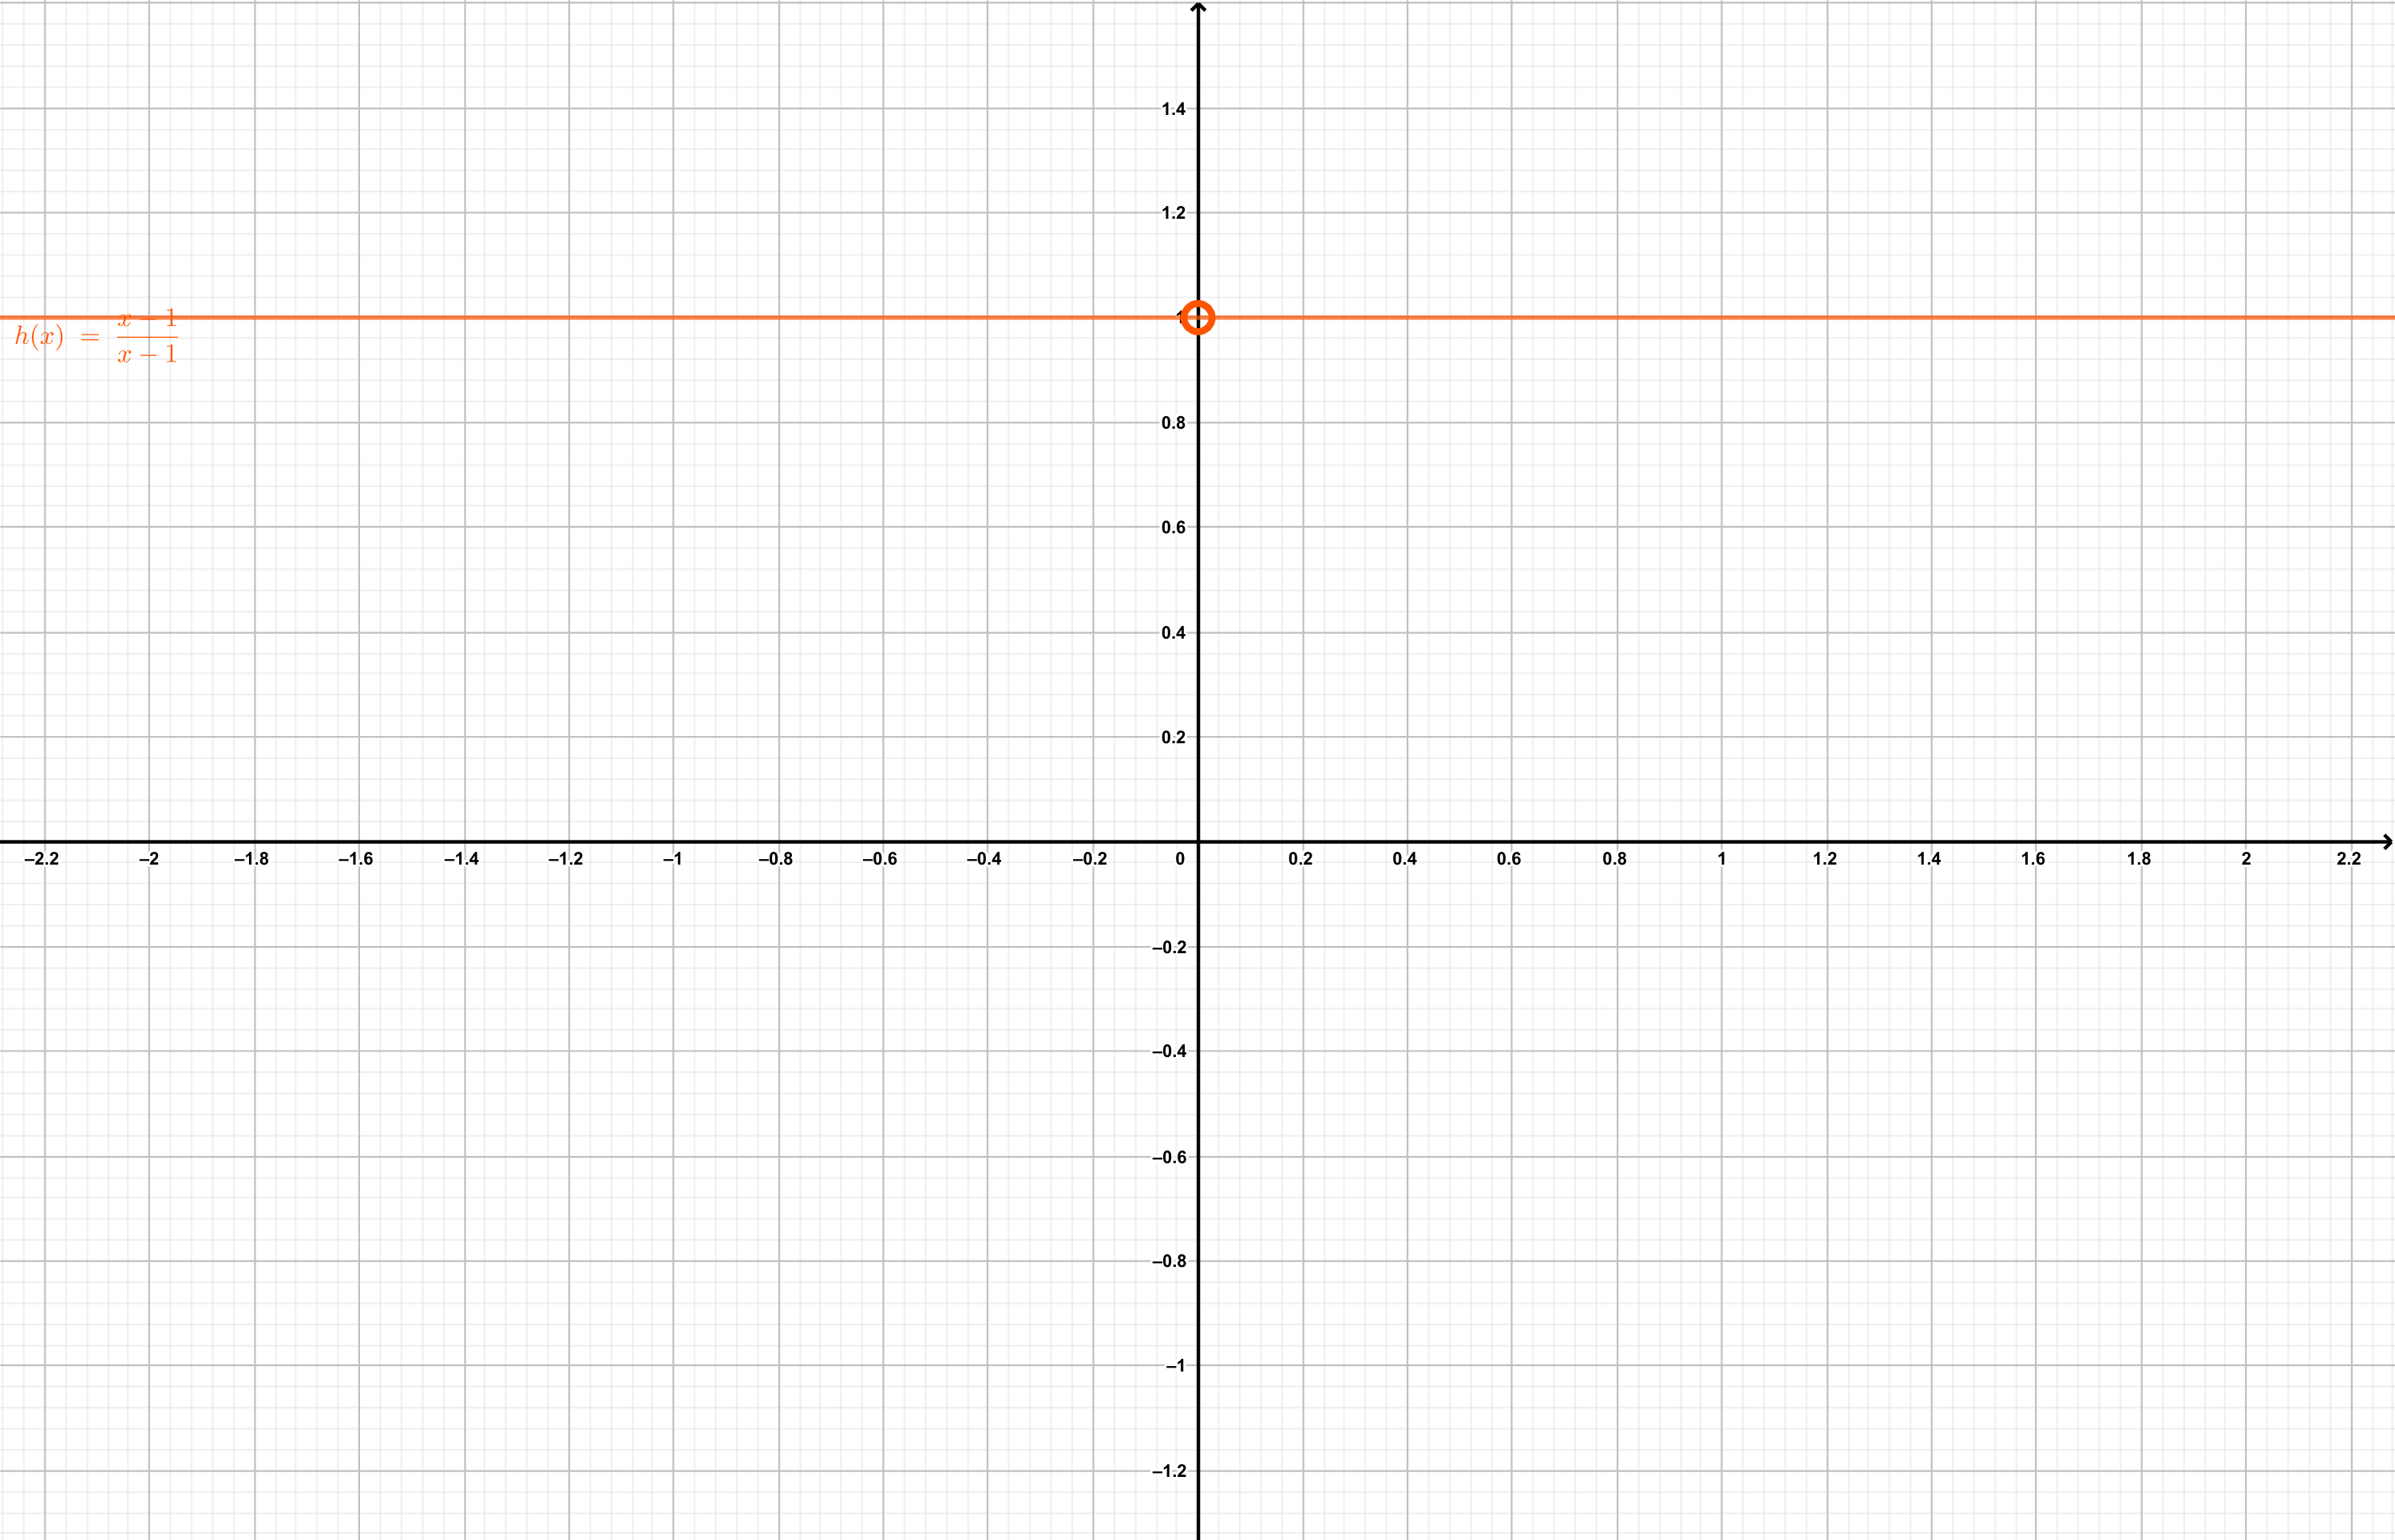
\includegraphics{Unidad-III/Func-discont} 

}

\caption{Ejemplo de función con discontinuidad.}\label{fig:discont}
\end{figure}

Hay funciones con discontinuidades, gráficamente más evidentes que \eqref{eq:disc-1}, como la hipérbola, \(f(x) = 1/x\) (figura \ref{fig:hiperb}) o \(g(x) = |x|/x\), o aquellas con condicionales.

\begin{figure}

{\centering 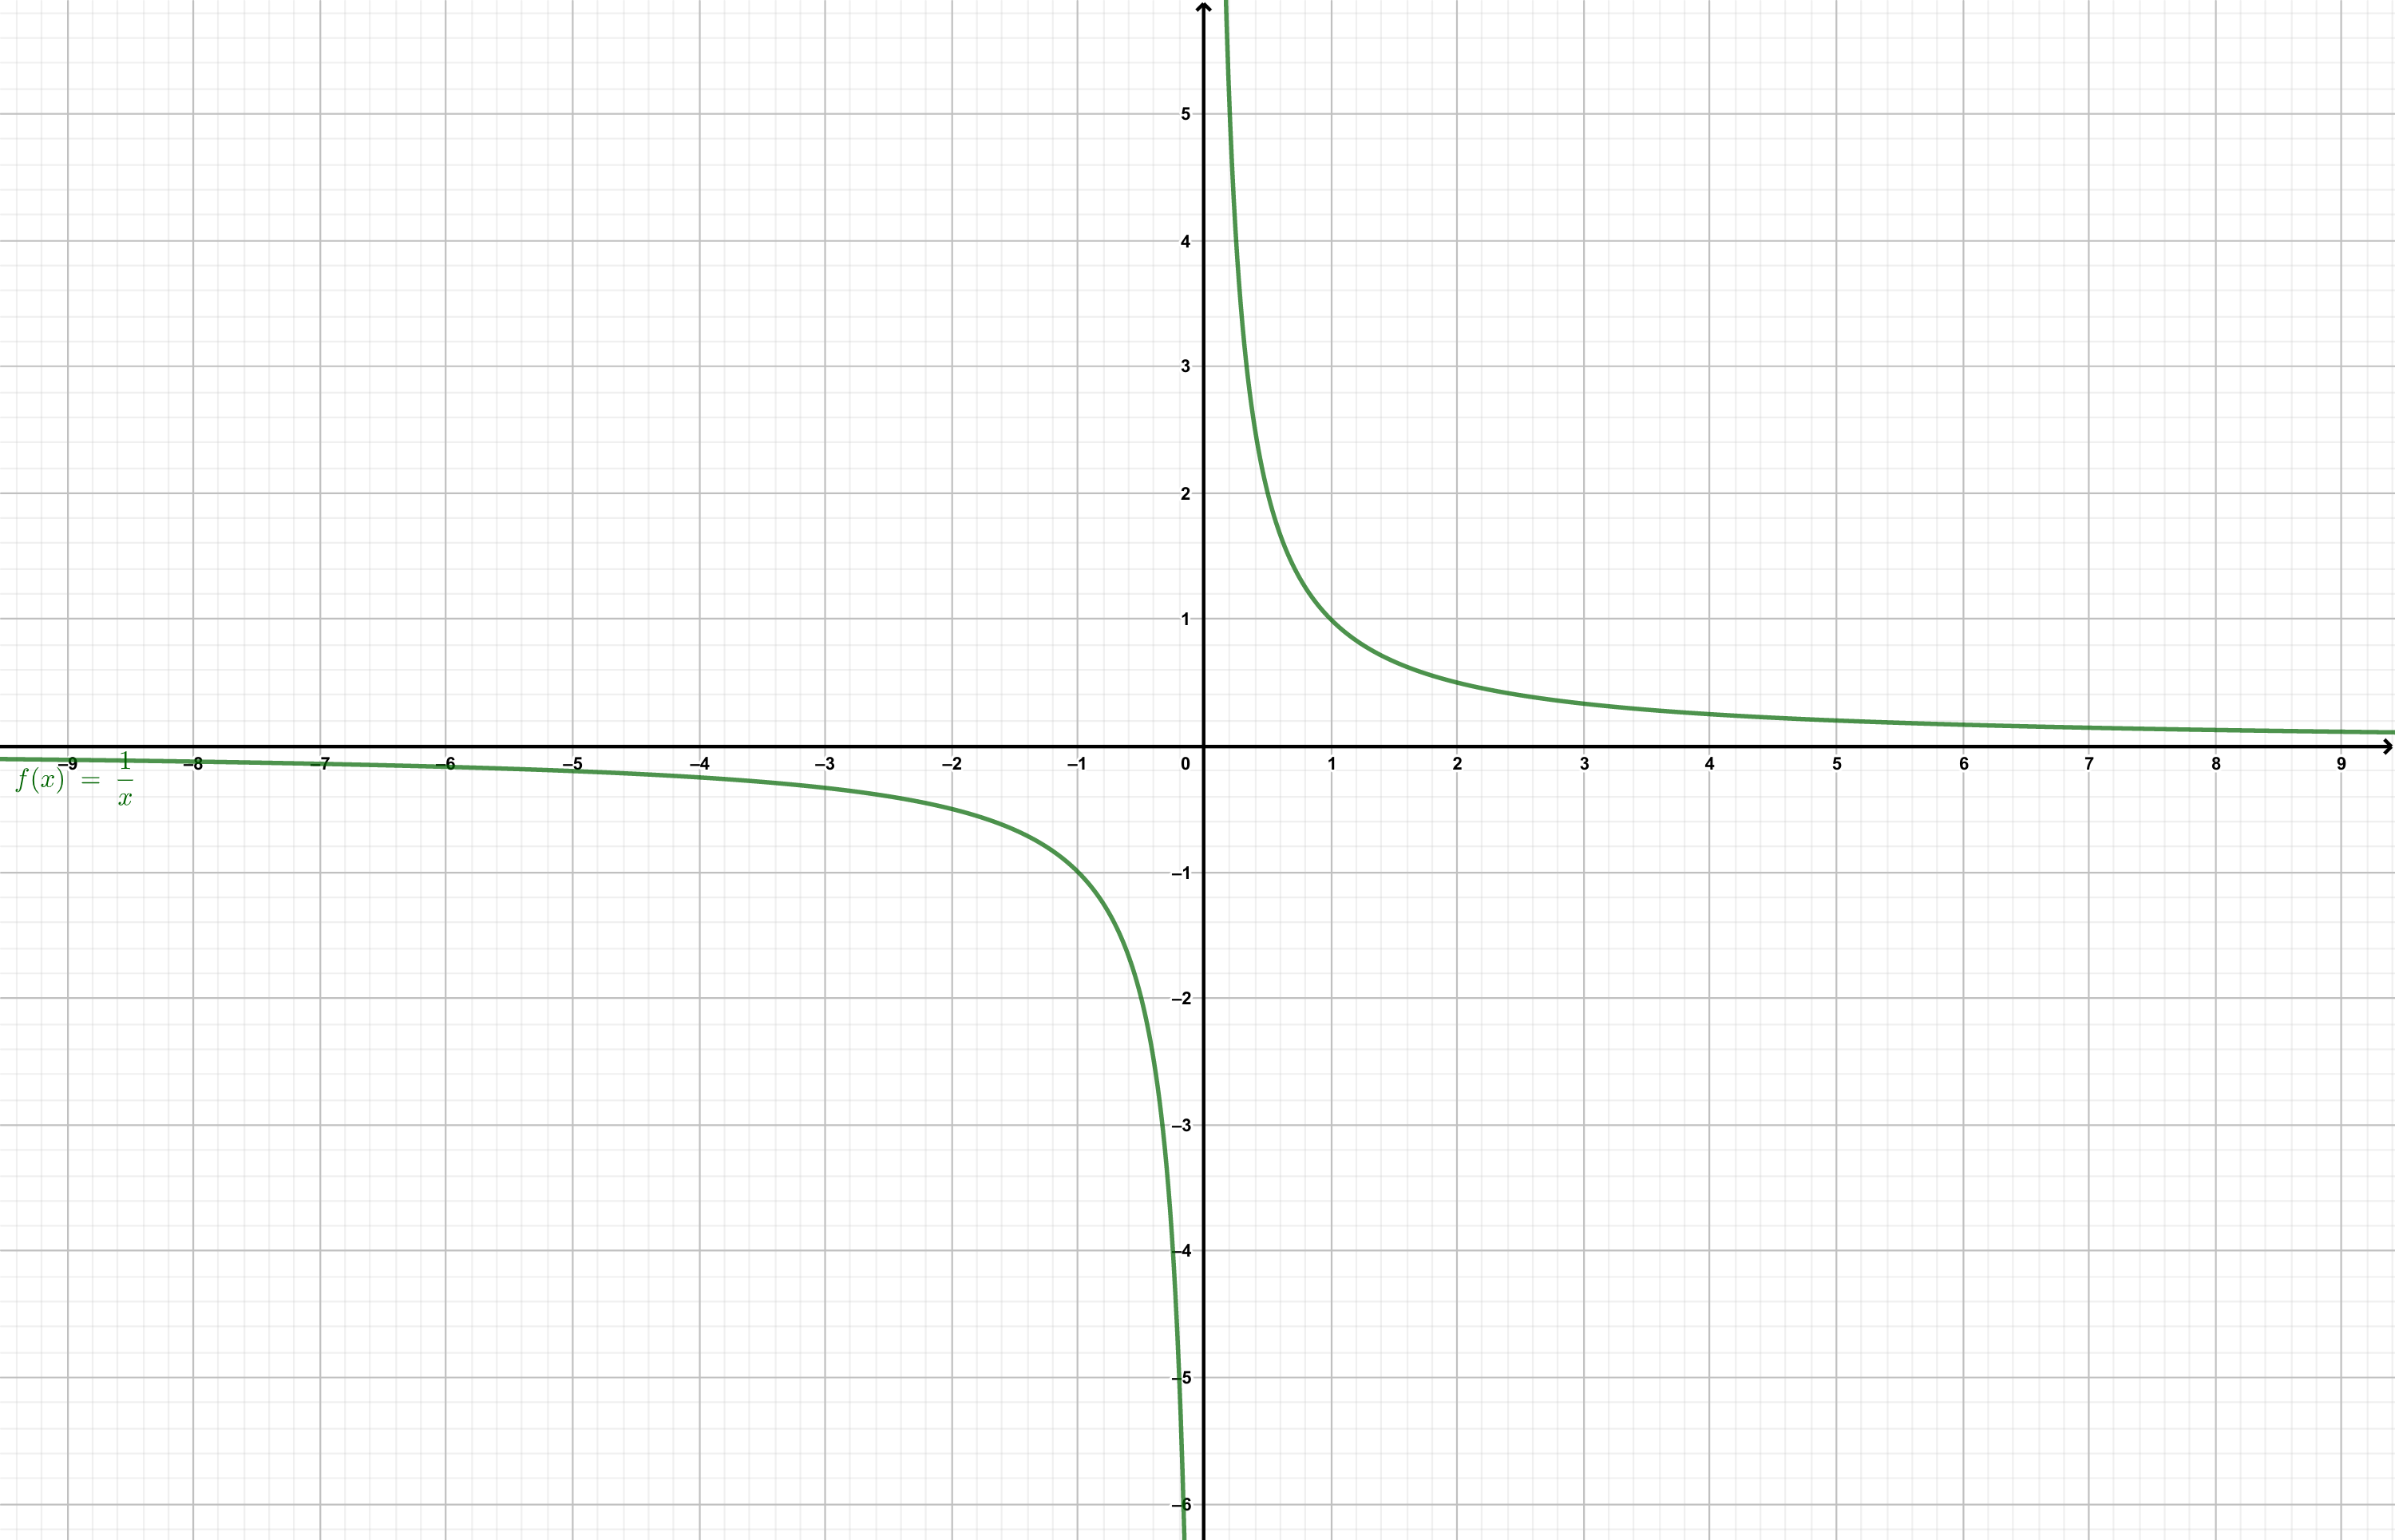
\includegraphics{Unidad-III/Hiperbola} 

}

\caption{La hipérbola.}\label{fig:hiperb}
\end{figure}

\begin{figure}

{\centering 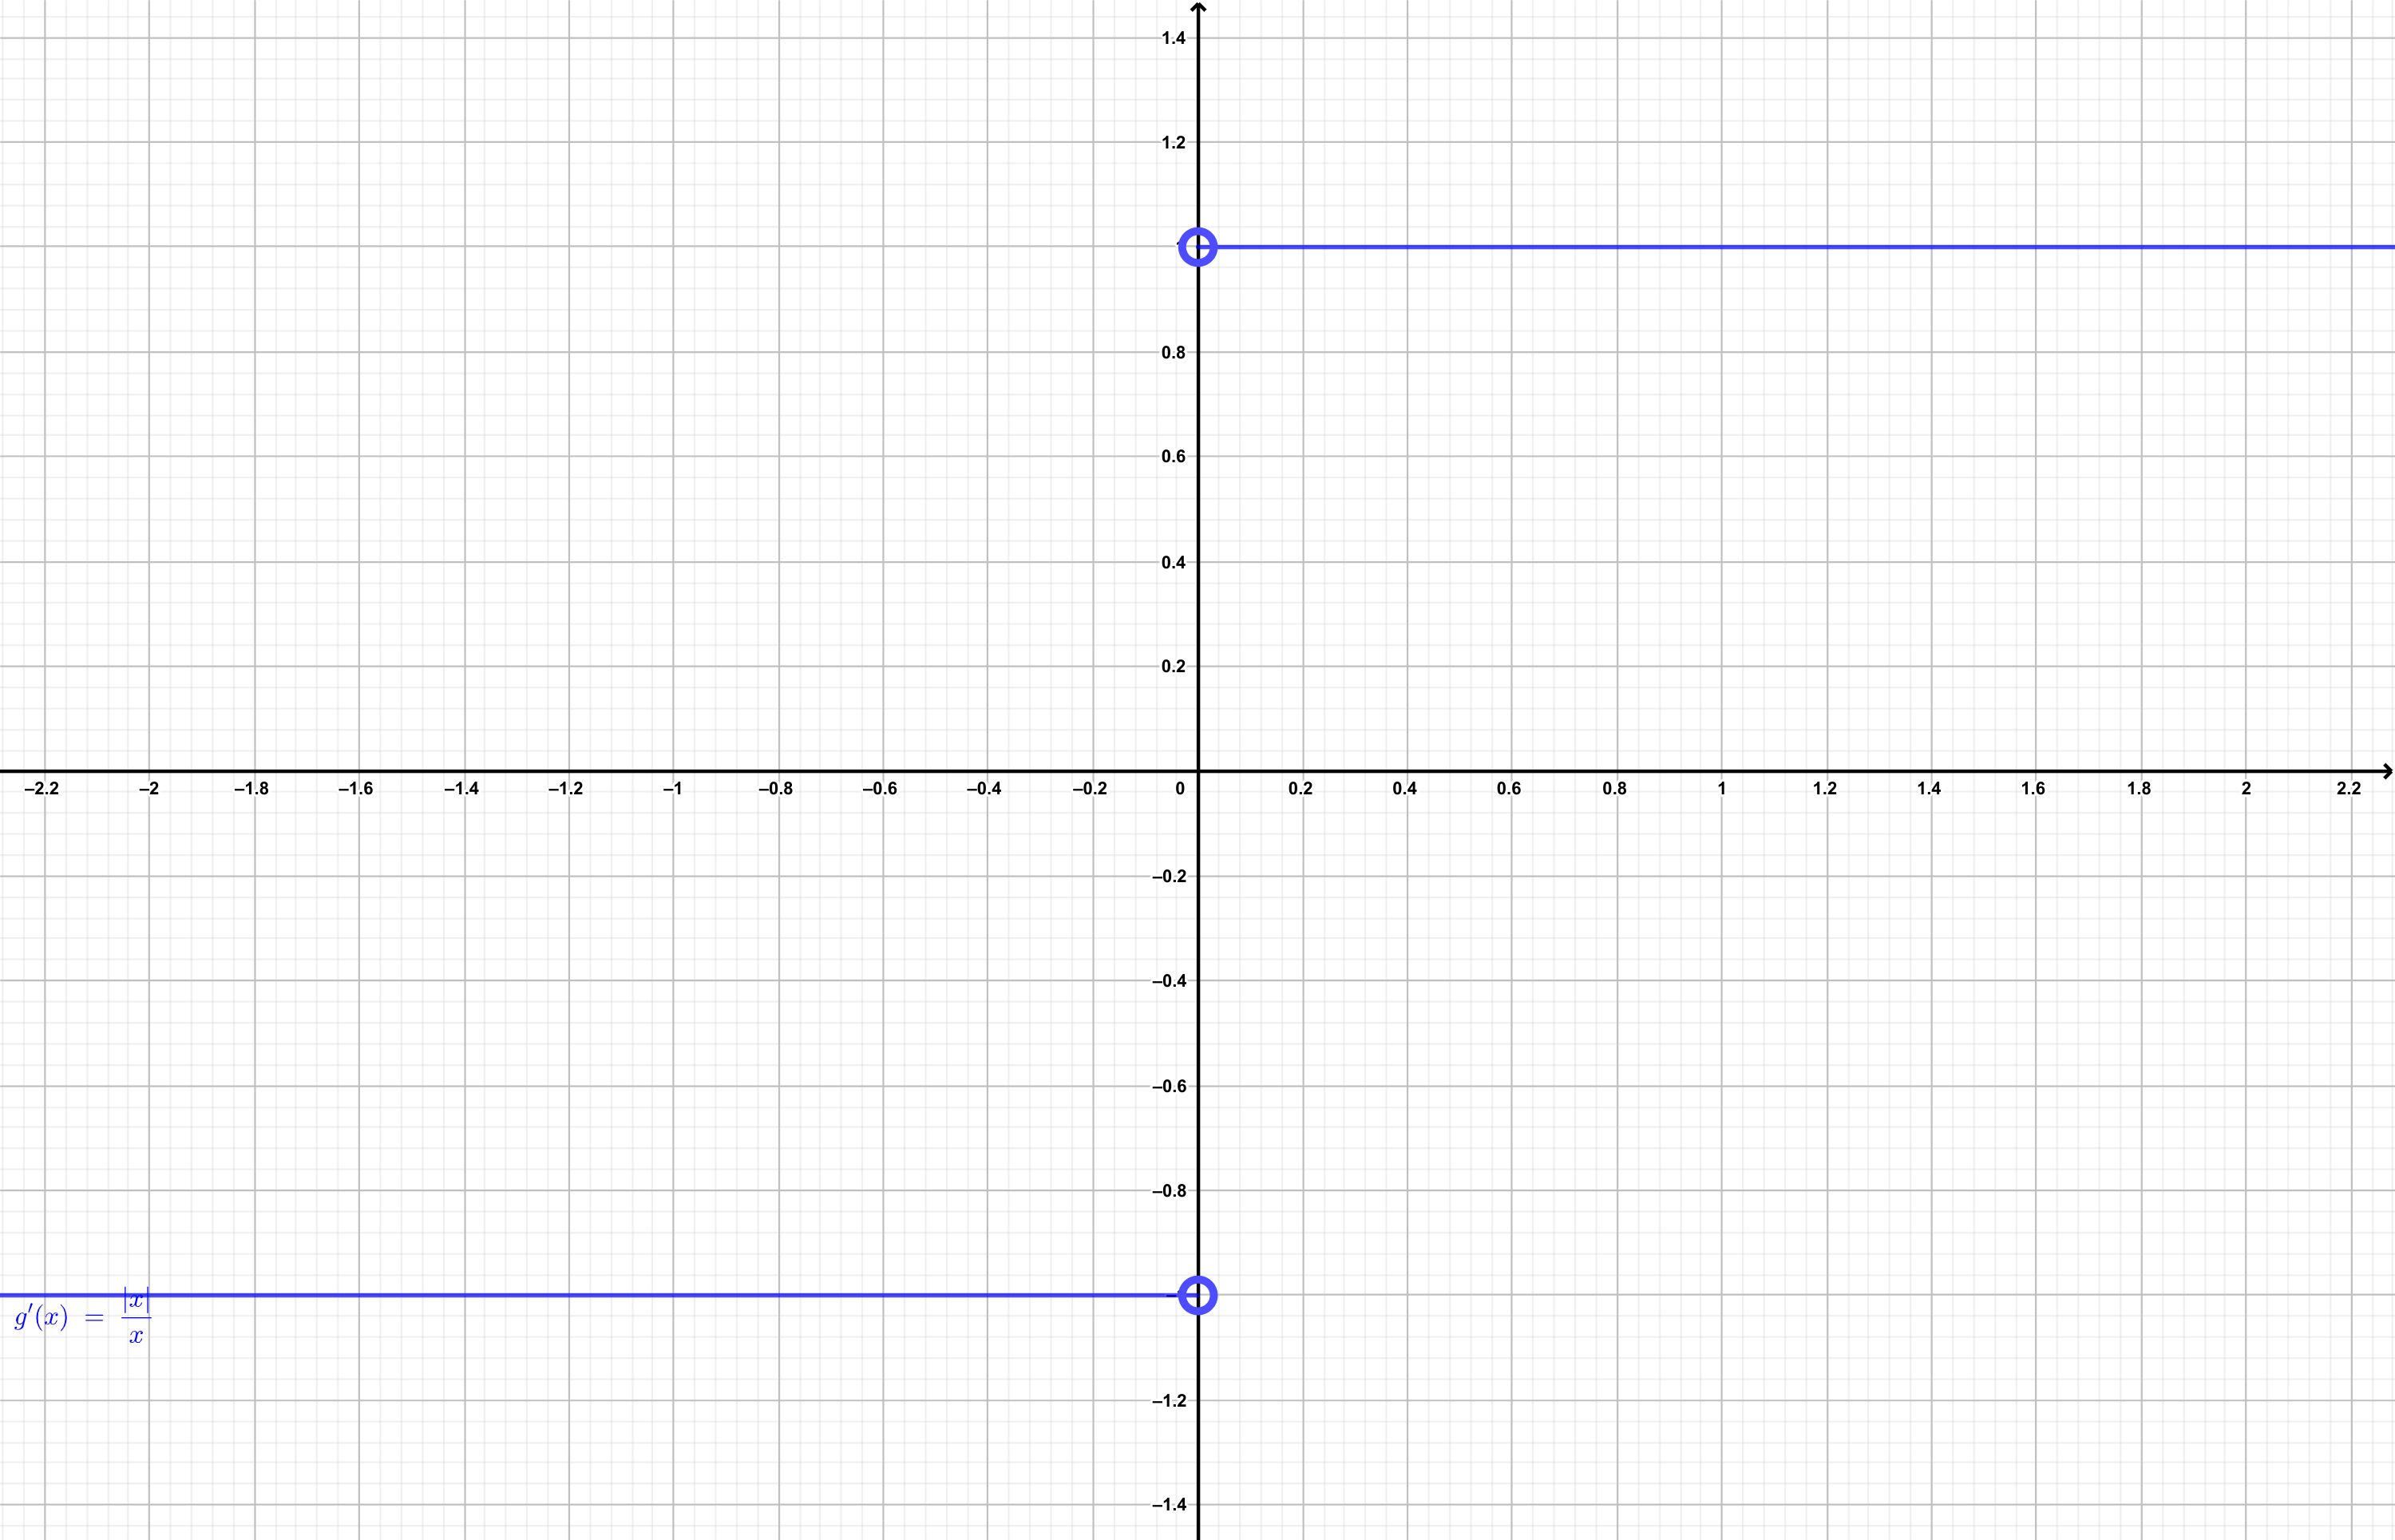
\includegraphics{Unidad-III/Deriv-absol} 

}

\caption{Cociente de valor absoluto.}\label{fig:absol}
\end{figure}

Como resulta geométricamente evidente, todas estas funciones son discontínuas para algún valor de \(x\), sin embargo existe una diferencia muy importante entre ellas y es que el valor que pueden tomar en torno al punto en que son discontínuas depende de qué lado nos acerquemos a este punto. Para la equación \(f(x) = \frac{x-1}{x-1}\), resulta claro que si nos acercamos a \(f(1)\) desde un valor \(x>1\), llegamos a un valor similar de \(f\) que si nos acercamos a \(f(1)\) por medio de un valor de \(x < 1\). Esto no sucede con las función \(g(x) = |x|/x\) puesto que si nos acercamos a \(g(0)\) por el lado positivo de \(x\) nos acercamos a \(g = 1\), mientras que, por el lado negativo, nos acercamos a \(g = -1\).

En este momento entonces es necesario comenzar a hablar del concepto de \textbf{límite}.

\hypertarget{el-luxedmite}{%
\subsection{El límite}\label{el-luxedmite}}

En el sentido estricto de la palabra, límite es el valor al que se acerca una función para un valor específico del dominio. En matemáticas, existe una notación específica para decir esto:

\begin{equation}
\lim \limits_{x \rightarrow a} x + 1
\end{equation}

donde \(\lim\) indica que necesitamos estimar el límite de la función, cuando su dominio \(x\) toma valores cada vez más cercanos a algún valor específico \(a\) (\(x \rightarrow a\)). Aquí es necesario especificar que cuando hablamos de límites \textbf{siempre} nos acercamos al valor de interés \(a\) tanto por medio de valores de \(x>a\) como \(x<a\), es decir alrededor de un intervalo de valores de \(x\) que comunmente se denomina como \(a \pm \delta\). Entonces, el límite de \(f(x)\) existe si todos los valores de \(f(a \pm \delta)\) convergen alrededor de un mismo punto.

Revisa la aplicación de Geogebra \href{https://www.geogebra.org/classic/b76f7gpx}{Límites} para visualizar este fenómeno. Juega con los valores de \(\delta\) y \(a\) para ver cómo están definidos los valores de la función alrededor de \(a\) para la función de la línea recta. Posteriormente, cambia la ecuación por:

\begin{enumerate}
\def\labelenumi{\arabic{enumi}.}
\tightlist
\item
  \(f(x) = \frac{|x|}{x}\)
\item
  \(f(x)= \frac{1}{x}\)
\end{enumerate}

para examinar qué pasa con \(f(x)\) cuando \(x \rightarrow 0\)

En los casos en que los valores de \(f(x)\) tienden a un valor único para \(f(a + \delta)\) y \(f(a - \delta)\), el límite de la función sí existe (figura \ref{fig:discont}). En cambio, como ocurre para funciones como \(1/x\) y \(|x|/x\), existe más de un valor al que ambas funciones se aproximan (figuras \ref{fig:hiperb} y \ref{fig:absol}) dependiendo se si se evalúa \(f(a + \delta)\) ó \(f(a - \delta)\), el límite no existe.

\begin{figure}

{\centering 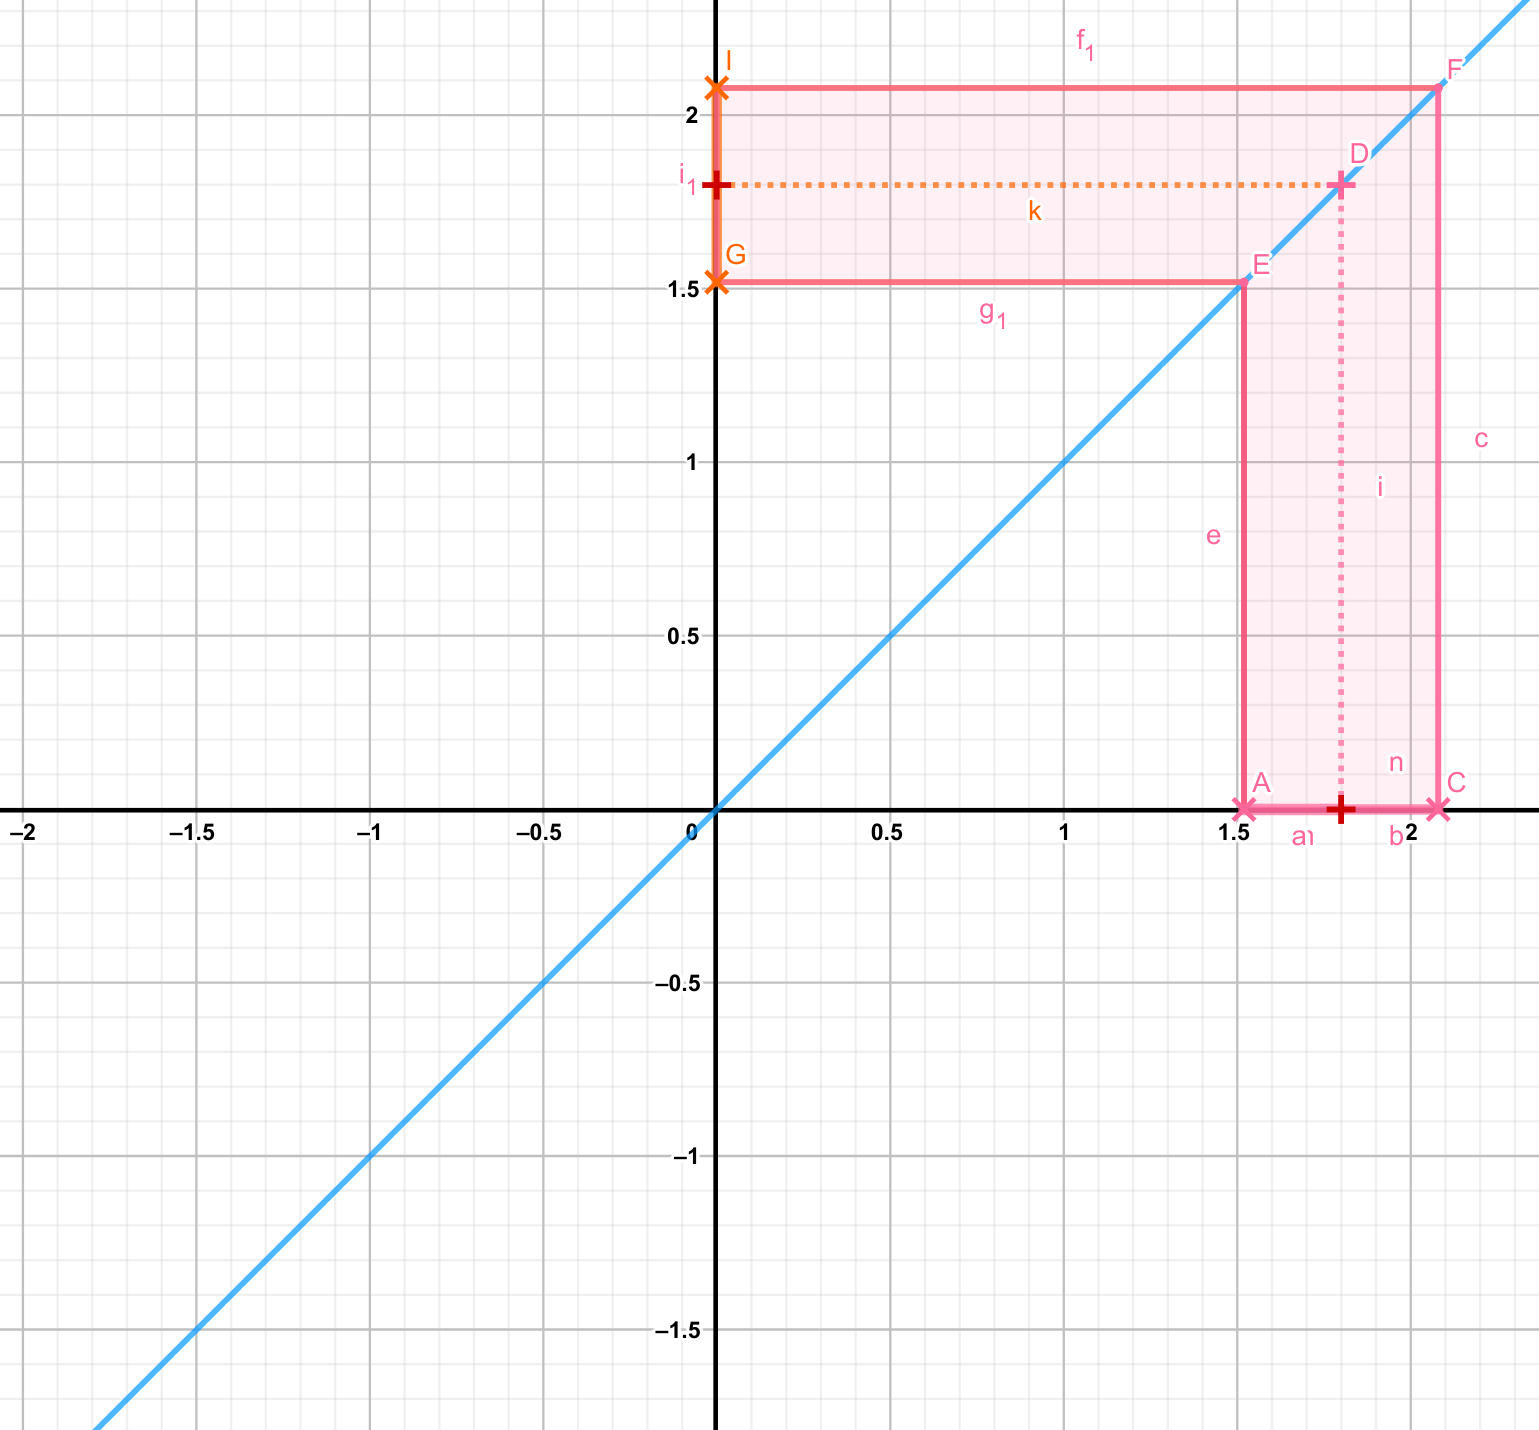
\includegraphics{Unidad-III/Limite-x} 

}

\caption{Ejemplo gráfico de una función con límite definido para cualquier valor de $x$. El valor $a$ al que $x$ se aproxima está marcado en el eje $x$ con una cruz roja, y el tamaño de ð alrededor de $a$ está delimitado con las marcas rosas. Nota cómo todos los valores posibles de $f(x)$ alrededor de $f(a)$ convergen en el mismo punto correspondiente a $f(a)$.}\label{fig:limite-def}
\end{figure}

\begin{figure}

{\centering 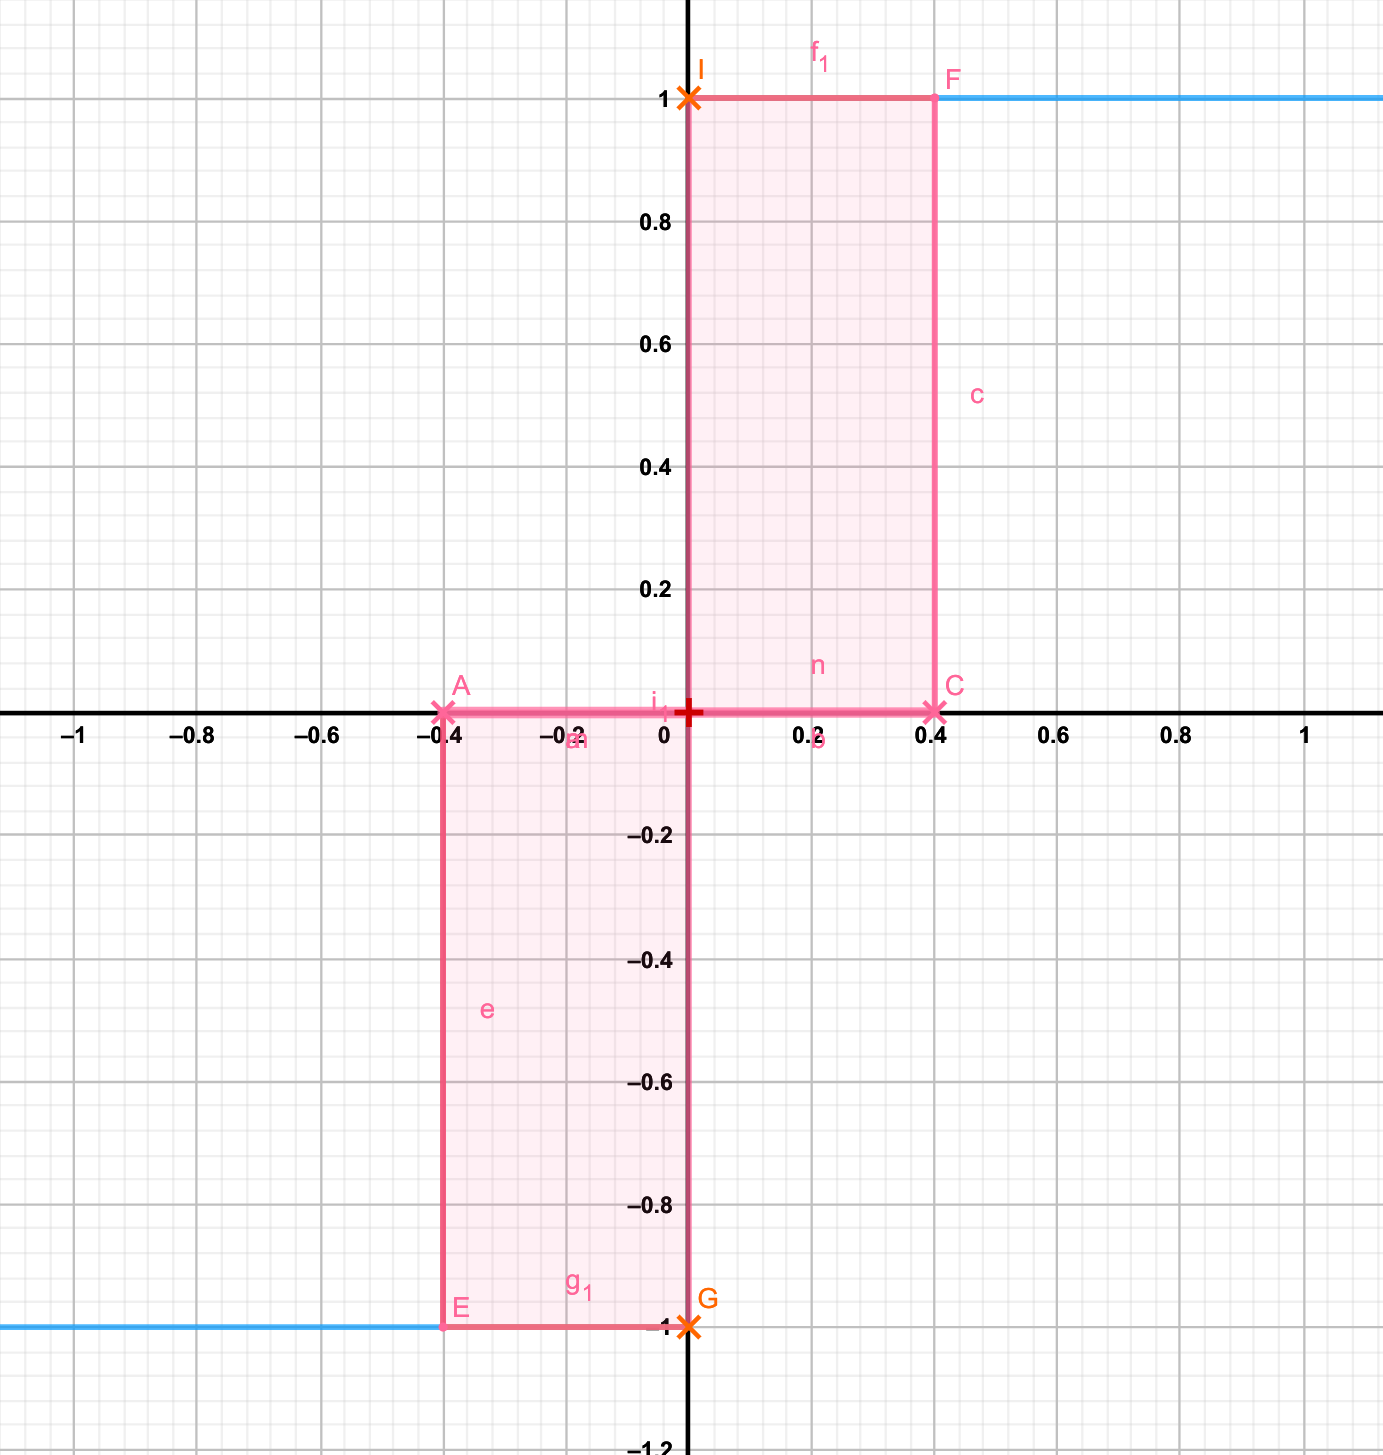
\includegraphics{Unidad-III/Limite-abs-x} 

}

\caption{Ejemplo gráfico de una función sin límite definido cuando x→0 (equis tiende a cero). Nota cómo hay dos valores posibles a los que la función se acerca cuando x→0, ya sea cuando uno se acerca a 0 por el lado positivo de $x$ o el lado negativo de $x$.}\label{fig:limite-indef}
\end{figure}

Aún cuando estas funciones no satisfacen la definición estricta de límite, es posible encontrar los límites de la función para \(f(a)\), dependiendo del lado por el que \(x \rightarrow a\). Veamos el ejemplo de \(f(x) = |x|/x\) dado en la figura \ref{fig:limite-indef}. El límite que nos interesa es

\[ \lim \limits_{x \rightarrow 0} \frac{|x|}{x}\]
Por lo que sabemos hay dos maneras que acercarnos a \(0\), una por el lado positivo, \(x \rightarrow 0^{+}\), y otra por el lado negativo \(x \rightarrow 0^-\). Así entonces podemos establecer dos límites:

\begin{enumerate}
\def\labelenumi{\arabic{enumi}.}
\tightlist
\item
  \(\lim \limits_{x \rightarrow 0^+} \frac{|x|}{x} = 1\)
\item
  \(\lim \limits_{x \rightarrow 0^-} \frac{|x|}{x} = -1\)
\end{enumerate}

\hypertarget{cuxf3mo-se-encuentran-los-luxedmites}{%
\subsubsection{¿Cómo se encuentran los límites?}\label{cuxf3mo-se-encuentran-los-luxedmites}}

Enncontrar límites puede ser problemático, por lo que existe una variedad de estrategias cuyo uso depende del tipo de expresión que estemos evaluando. Por lo general, si tenemos \(\lim\limits_{x \rightarrow a} f(x)\) se puede comenzar por evaluar \(f(a)\), con lo que tenemos tres posibilidades:

\begin{enumerate}
\def\labelenumi{\arabic{enumi}.}
\tightlist
\item
  \(f(a) = \frac{b}{0}, b \neq 0\) (una asíntota vertical como en \(1/x\))
\item
  \(f(a) = b\) (límite encontrado)
\item
  \(f(a) = \frac{0}{0}\) (indeterminación)
\end{enumerate}

En el caso \textbf{1}, es probable que el límite no exista, lo cual depende de que \(\lim\limits_{x \rightarrow a^-} f(x) = \lim\limits_{x \rightarrow a^+} f(x)\). Para el caso \textbf{2}, el límite está claramente definido y no hay mayor problema. En el caso \textbf{3}, es necesario encontrar una manera equivalente de representar a \(f(a)\).

\hypertarget{representaciuxf3n-equivalente-de-las-funciones}{%
\subsubsection{Representación equivalente de las funciones}\label{representaciuxf3n-equivalente-de-las-funciones}}

Las tres estrategias más comunes para resolver límites donde \(f(a) = \frac{0}{0}\) son:

\begin{enumerate}
\def\labelenumi{\arabic{enumi}.}
\tightlist
\item
  Factorizar \(f(a)\)
\item
  Conjugar \(f(a)\)
\item
  Usar identidades trigonométricas
\end{enumerate}

Cabe aclarar que muchas de las transformaciones aquí descritas surten efecto bajo el supuesto de que \(x \neq a\), aunque una vez transformadas las funciones en efecto las evaluamos asumiendo que \(x = a\). Con esto en mente veamos un ejemplo para cada estrategia.

\hypertarget{factorizaciuxf3n}{%
\paragraph{Factorización}\label{factorizaciuxf3n}}

Factorizar consiste en representar un polinomio como una serie de productos de binomios (generalmente). Así, por ejemplo:

\begin{equation}
    \lim \limits_{x \rightarrow -3} \frac{x^2 + x -6}{x + 3}
\end{equation}

por sustitución directa tenemos que

\begin{equation}
\frac{(-3)^2 - 3 - 6}{-3 + 3} = \frac{0}{0}
\end{equation}

Y una vez factorizado, asumiendo que \(x \neq 3\) tenemos

\begin{equation}
 \frac{x^2 + x - 6}{x + 3} = \frac{(x + 3)(x - 2)}{x + 3} = x-2
 \end{equation}

por lo tanto, utilizando sustitución directa en la forma factorizada tenemos que:

\begin{equation}
 \lim\limits_{x \rightarrow 3} x - 2 = - 3 - 2 = -5
\end{equation}

\hypertarget{conjugaciuxf3n-racional}{%
\paragraph{Conjugación racional}\label{conjugaciuxf3n-racional}}

Una expresión conjugada de un binomio está basada en la identidad:

\[ a^2 - b^2 =(a + b)(a - b)\]

Esta identidad se puede extender a los radicales:

\[ a - b = (\sqrt{a} + \sqrt{b})(\sqrt{a} - \sqrt{b})\]

De modod que el conjugado de \(a + b\) es \(a-b\), y el de \(\sqrt{a} + \sqrt{b}\) es \(\sqrt{a} - \sqrt{b}\).

La aplicación de conjugados entonces es particularmente útil cuando queremos evaluar un el límite de una funcion racional con radicales. Por ejemplo en:

\begin{equation}
\lim \limits_{x \rightarrow 0} \frac{\sqrt{1 + x}-1}{x}
\end{equation}

por sustitución directa obtenemos \frac{0}{0}, pero no es posible factorizar el numerador, por lo tanto podemos utilizar el conjugado de \(\sqrt{1 + x} - 1\). La manera de hacerlo es, primero identificar el cojugado como:

\begin{equation}
    \sqrt{1 + x} + 1
\end{equation}

Y multiplicar tanto el nuemerados como denominador por el conjugado:

\begin{equation}
  \frac{\sqrt{1 + x}-1}{x} \cdot  \frac{\sqrt{1 + x} + 1}{\sqrt{1 + x} + 1} = \frac{1 + x-1}{x(\sqrt{1 + x} + 1)} = \frac{1}{\sqrt{1 + x} + 1}
\end{equation}

Con lo que ya podemos evaluar:

\begin{equation}
\lim\limits_{x \rightarrow 0} \frac{1}{\sqrt{1 + x} + 1} = \frac{1}{1 + 1} = \frac{1}{2}
\end{equation}

\hypertarget{identidades-trigonomuxe9tricas}{%
\paragraph{Identidades trigonométricas}\label{identidades-trigonomuxe9tricas}}

Cuano es necesario evaluar el límite de una función trigonométrica, es útil echar mano de las identidades, además de las ya bien conocidas, las pitagóricas:

\begin{enumerate}
\def\labelenumi{\arabic{enumi}.}
\tightlist
\item
  \(\mathrm{sen}^2 \theta + \cos^2 \theta = 1\)
\item
  \(\sec^2 \theta - \tan^2 \theta = 1\)
\item
  \(\csc^2 \theta - \cot^2 \theta = 1\)
\end{enumerate}

Comencemos por ver un ejemplo basado en las identidades basadas en los cocientes.

\begin{equation}
\lim \limits_{x \rightarrow 0} \frac{3x \tan x}{\mathrm{sen}x}
\end{equation}

por sustitución directa tenemos que:

\begin{equation}
\frac{3(0)\tan 0}{\mathrm{sen} 0} = \frac{0}{0}
\end{equation}

lo que indica que necesitamos representar a la función de una manera alternativa, echando mano de las identidades. Sabemos que:

\begin{equation}
\tan \theta = \frac{\mathrm{sen} \theta}{\cos \theta}
\end{equation}

por lo tanto podemos representar la función como:

\begin{equation}
\frac{3x \tan x}{\mathrm{sen}x} = \frac{3x \mathrm{sen} x}{\cos^2 x} = \frac{3x}{\cos x}
\end{equation}

Entonces, tenemos el límite que puede ser evaluado por sustitución directa:

\begin{equation}
\lim \limits_{x \rightarrow 0} \frac{3x}{\cos x} = \frac{3(0)}{\cos 0} = \frac{0}{1} = 0
\end{equation}

\hypertarget{equivalencias-de-luxedmites}{%
\subsubsection{Equivalencias de límites}\label{equivalencias-de-luxedmites}}

Los límites, como hemos visto, son números reales, por lo que todos los axiomas que ya conocemos aplican a los números reales:

\begin{enumerate}
\def\labelenumi{\arabic{enumi}.}
\item
  \(\lim \limits_{x \rightarrow a} f(x) + g(x) = \lim \limits_{x \rightarrow a} f(x) + \lim \limits_{x \rightarrow a} g(x)\)
\item
  \(\lim \limits_{x \rightarrow a} f(x) \cdot g(x) = \lim \limits_{x \rightarrow a} f(x) \cdot \lim \limits_{x \rightarrow a} g(x)\)
\item
  \(\lim \limits_{x \rightarrow a} \frac{f(x)}{g(x)} = \frac{\lim \limits_{x \rightarrow a} f(x) }{ \lim \limits_{x \rightarrow a} g(x)}\)
\item
  \(\lim \limits_{x \rightarrow a} c f(x) = c \lim \limits_{x \rightarrow a} f(x)\)
\item
  \(\lim \limits_{x \rightarrow a} f(x)^2 = \left( \lim \limits_{x \rightarrow a} f(x) \right)^2\)
\end{enumerate}

\hypertarget{derivaciuxf3n}{%
\section{Derivación}\label{derivaciuxf3n}}

Hasta el momento hemos mencionado en repetidas ocasiones una serie de conceptos relacionados muy íntimamente con la derivación. En esencia, en cálculo, el proceso de derivación se utiliza para estimar la pendiente de una recta tangente a un punto cualquiera que forma parte de una función (Figura \ref{fig:deriv}).

\begin{figure}

{\centering 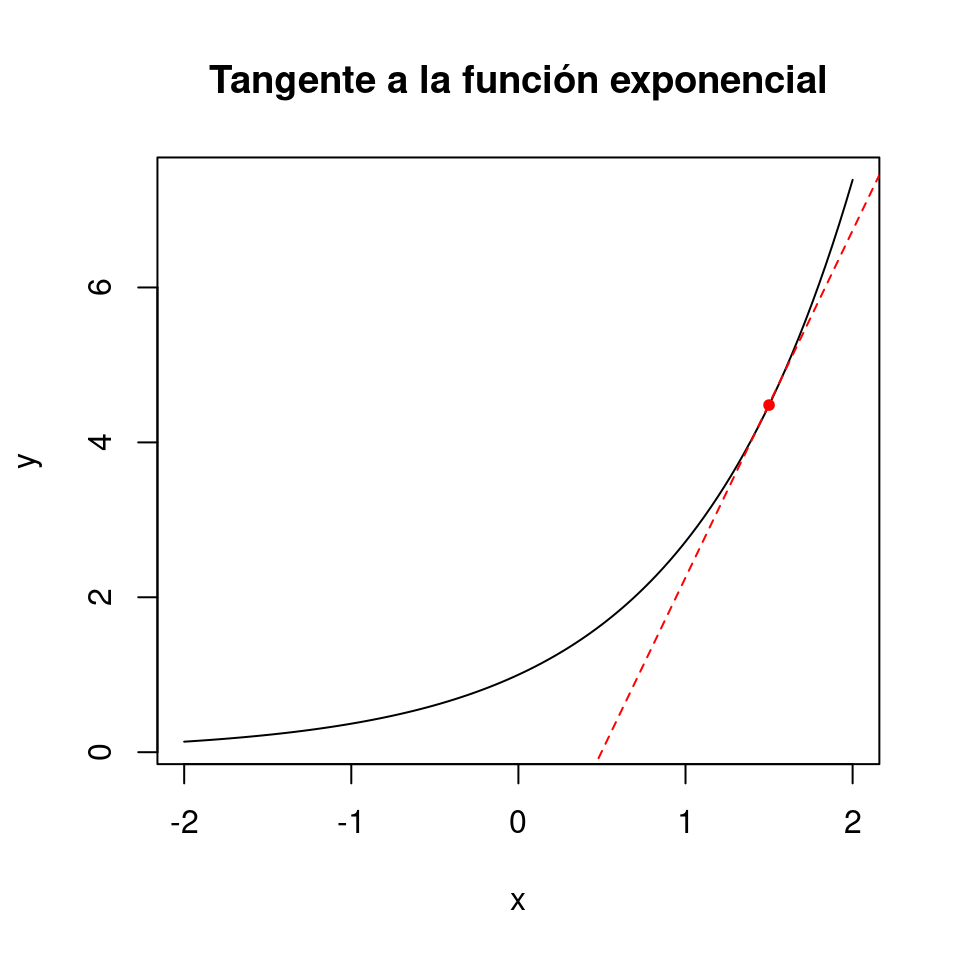
\includegraphics{Model-mate_files/figure-latex/deriv-1} 

}

\caption{Representación gráfica de la tangente a un punto en la curva exponencial.}\label{fig:deriv}
\end{figure}

El proceso de estimar la pendiente de una tangente a la función en un punto \((x, f(x))\) consiste en estimar el límite:

\begin{equation}
\lim \limits_{h \rightarrow 0} \frac{f(x + h) - f(x)}{x - (x + h)} \label{eq:derivada}
\end{equation}

Resolverlo no requiere de un conocimiento profundo para encontrar que por sustitución directa de \(h = 0\), se obtiene una undeterminación (\(0/0\)). Sin embargo para entender mejor de qué se trata el límite de la ecuación \eqref{eq:derivada} podemos explorarlo con la \href{https://www.geogebra.org/classic/rjttr8kq}{aplicación para derivadas}.

\hypertarget{ejemplos-1}{%
\subsection{Ejemplos}\label{ejemplos-1}}

\hypertarget{ecuaciuxf3n-cuadruxe1tica}{%
\subsubsection{Ecuación cuadrática:}\label{ecuaciuxf3n-cuadruxe1tica}}

\[ y = x^2\]
Con lo que la derivada sería:

\begin{equation}
\lim \limits_{h \rightarrow 0} \frac{(x + h)^2 - x^2}{(x+h) - x}
\end{equation}

Utilizando las técnicas para resolver límites podemos que con este último se puede utilizar factorización para obtener:

\begin{equation}
\lim \limits_{h \rightarrow 0} \frac{(x + h)^2 - x^2}{(x+h) - x} = \lim \limits_{h \rightarrow 0} \frac{((x + h) - x)((x + h) - x)}{(x + h) + x} = \lim \limits_{h \rightarrow 0} (x + h) + x = \lim \limits_{h \rightarrow 0} 2x + h
\end{equation}

Con este resultado podemos ahora sí sustituir \(h\) directamente para ver que la derivada \(y' = 2x\).

\hypertarget{hiperbola}{%
\subsubsection{Hiperbola}\label{hiperbola}}

\[ y = \frac{1}{x}\]
Derivada:

\begin{equation}
\lim \limits_{h \rightarrow 0} \frac{\frac{1}{x + h} - \frac{1}{x}}{(x+h) - x}
\end{equation}

Podemos comenzar por simplificar las fracciones:

\begin{equation}
\lim \limits_{h \rightarrow 0} \frac{\frac{x - (x + h)}{x(x + h)}}{h} = \lim \limits - \frac{h}{x^2 + xh} \frac{1}{h} = \lim \limits_{h \rightarrow 0} -\frac{1}{x^2}
\end{equation}

Por lo tanto \(y' = \frac{1}{x^2}\)

\hypertarget{notaciuxf3n}{%
\subsection{Notación}\label{notaciuxf3n}}

La técnica de derivación se le atribuye a dos científicos, Isaac Newton y Gottfried Leibniz. La notación que se tradicionalmente enseña para comenzar con cáculo es la de Newton:

\begin{equation}
f'(x) = \lim \limits_{h \rightarrow 0} \frac{f(x + h) - f(x)}{h} \label{eq:Newton}
\end{equation}

la cual adolece de claridad, pues a menos que uno conozca bien la fórmula de la derivada no especifica el significado de \(f'(x)\). La notación de Leibniz en cambio, sí lo especifica:

\begin{equation}
\frac{df}{dx} = f'(x) \label{eq:Leibniz}
\end{equation}

donde el numerador \(df = \Delta f = f(x + h) - f(x)\) y el denominador \(dx = \Delta x = (x+h) - x = h\). La letra \(d\) se utiliza en lugar de \(\Delta\) para indicar que se trata de un cambio contínuo, en lugar de discreto, el uso tradicional de \(\Delta\).

\hypertarget{reglas-de-derivaciuxf3n}{%
\subsection{Reglas de derivación}\label{reglas-de-derivaciuxf3n}}

\hypertarget{potencias}{%
\subsubsection{Potencias}\label{potencias}}

Como ya se habrán dado cuenta, la primera regla de la derivación está relacionada con los exponentes. Por ejemplo, la derivadas de \(f(x) = x^2\) y \(f(x) = \frac{1}{x}\), son \(\frac{df}{dx} = 2x\) y \(\frac{df}{dx} = - \frac{1}{x^2}\) respectivamente. Nota, que en ambos casos, los exponentes de cada \(x\), se convirtieron en coeficientes en \(\frac{df}{dx}\), y que restamos \(1\) a cada exponente de \(x\):

\begin{enumerate}
\def\labelenumi{\arabic{enumi}.}
\tightlist
\item
  \(x^2 \rightarrow 2x^{2-1} = 2x^1 = 2x\)
\item
  \(1/x = x^{-1} \rightarrow -1x^{-1-1} = -x^{-2} = - 1/x^2\)
\end{enumerate}

Entonces la primera regla de la derivación, se puede aplicar a muchas funciones. Si \$f(x) = x\^{}n \$, \$\frac{df}{dx} = nx\^{}\{n-1\} \$.

En casos donde \(x\) aparece más de una vez, se considera que:

\[f(x) = f_1(x) + f_2{x} + \dots + f_n(x)\]

Y dado que la derivada es un límite, sabemos que \(f'(x) = f'_1(x) + f'_2(x) + \dots + f'_n(x)\).

Por ejemplo, si tenemos la función

\[y = a + bx + cx^2 + dx^3 = ax^0 + bx^1 + cx^2 + dx^3\]

su derivada será

\[ \frac{dy}{dx} = 0ax^{0-1} + bx^{1-1} + 2cx^{2-1} + 3dx^{3-1}= b + 2cx + 3dx^2\]

\hypertarget{productos}{%
\subsubsection{Productos}\label{productos}}

Si \(h(x) = f(x)g(x)\) entonces:
\[h'(x) = f'(x)g(x) + f(x)g'(x)\]

\hypertarget{cocientes}{%
\subsubsection{Cocientes}\label{cocientes}}

Si \(h(x) = \frac{f(x)}{g(x)}\), entonces:

\[h'(x) = \frac{f'(x)g(x) - f(x)g'(x)}{g(x)^2}\]

\hypertarget{funciones-en-cadena}{%
\subsubsection{Funciones en cadena}\label{funciones-en-cadena}}

Una función en cadena es aquella en que \(h(x) = (f \circ g)(x) = f(g(x))\), entonces:

\[h'(x) = f'(g(x))g'(x) = (f \circ g)'(x) g'(x)\]

Aquí es preciso dar un ejemplo:

\[h(x) = (3x-1)^2\]

donde está claro que \(g(x) = 3x^2-1\) y que \(f(u) = u^2\). Por lo tanto si evaluamos \(f'(u)\) cuando \(u = 3x^2-1\), entonces \(f'(u) = 2(3x^2-1)\). Por el otro lado, tenemos que, aplicando la regla de las potnecias, \(g'(x) = 6x\). Entonces:

\[h'(x) = 2(3x^2-1)6x\]

\hypertarget{representaciuxf3n-geomuxe9trica-de-la-derivada}{%
\subsection{Representación geométrica de la derivada}\label{representaciuxf3n-geomuxe9trica-de-la-derivada}}

Como resultado del proceso de derivación de una función \(f(x)\) se obtiene una segunda función \(f'(x)\) ó \(\frac{d}{dx}f\) cufo valor corresponde a la pendiente de una tangente para cada par de valores \((x, f(x))\).

La aplicación \href{https://www.geogebra.org/classic/w3spjhc7}{Interpretación de la derivada}, muestra ambas funciones y la recta tangente a \((x,f(x))\). Observa la pendiente de esta tangente y las coordenadas \((x, f'(x))\).

\hypertarget{aplicaciones}{%
\subsection{Aplicaciones}\label{aplicaciones}}

Uno de los modelos más generalizables que se utilizan en ecología es el de crecimiento exponencial:

\[N(t) = e^{rt}\]

Como vimos anteriormente, este modelo se puede linealizar utilizando el logaritmo:

\begin{equation}
\ln N(t) = rt \label{eq:log-N}
\end{equation}

y si resolvemos para \(r\), obtenemos que:

\[r = \frac{\ln N}{t}\]

la pendiente, o tasa de crecimiento de una poblaciones equivalente a \(\ln N/t\), para cualquier período de tiempo. Volvamos sin embargo a la ecuación \eqref{eq:log-N}, diferenciándola. Para esto utilizaremos la diferenciación implícita, pues necesitamos conocer:

\begin{enumerate}
\def\labelenumi{\arabic{enumi}.}
\tightlist
\item
  \(\frac{d}{dt}rt = r\)
\item
  \(\frac{d}{dt}N(t) \ln N = \frac{d}{dt} \frac{1}{N}\)
\end{enumerate}

por lo tanto:

\[\frac{dN}{dt} \frac{1}{N} = t\]

Con lo que obtenemos la siguiente ecuación diferencial:

\begin{equation}
\frac{dN}{dt} = rN
\end{equation}

De este modo podemos ver que, el crecimiento instantáneo de una población durante el intervalo \(dt\) es equivalente a la tasa de crecimiento exponencial \(r\). Más adelante veremos por qué \(f(x) = \ln x\), \(f'(x) = 1/x\), por el momento esta equivalencia nos sirve para ver que si \(N(t) = e^{rt}\):

\[\frac{dN}{dt} = e^{rt} = rN\]
Y si separamos ambos lados \(N\) y \(t\), tenemos:

\[\frac{dN}{N} = r \cdot dt\]

Por lo tanto, la derivada nos sirve para estudiar de cerca la tasa de crecimiento en relación al cambio de población \(dN\) y de tiempo \(dt\), con un modelo lineal.

\hypertarget{integraciuxf3n}{%
\section{Integración}\label{integraciuxf3n}}

La integración es el proceso de estimación del área bajo la curva de una función, y para nosotros como ecólogxs es muyimportante, pues la mayoría de los modelos dinámicos se formulan como ecuaciones diferenciales, los cuales debemos integrar para obtener las soluciones.

Al igual que con límites y derivadas, hay toda una notación particular de la integración:

\begin{equation}
    \int_a^b \!f(x) dx
\end{equation}

Y se lee, la integral de \(f(x)\) entre \(a\) y \(b\). \([a, b]\) corresponde a dos valores, mínimo (\(a\)) y máximo (\(b\)), de \(x\) entre los cuales se evaluará el área. El símbolo \(\int\), es una ``S'', e indica la suma de valores contínuos. Al igual que en la derivada, el signo \(d\) es la versión contínua de \(\Delta\), en las integrales \(\int\) es la versión contínua de \(\sum\).

Otra similitud entre la dericada y la integral es que est última es un límite:

\begin{equation}
    \int_a^b \!f(x) dx = \lim \limits_{n \rightarrow \infty} \sum_{i = 1}^n f(x_i) \Delta x; \Delta x = \frac{b-a}{n} \label{eq:integ-limite}
\end{equation}

Para comprederla, enfoquémonos en el lado derecho, que comenzando con el operador de sumatoria \(\sum\) indica que para cada valor \(x_i\), se evalúa la función \(f\), y se multiplica por la distancia que hay entre \(x_i\) y \(x_{i-1}\) (\(\Delta x\)). Si pensamos esto en el plano cartesiano, \(f(x_i)\) es la distancia entre \(0\) y el valor de \(y\) en \(f(x_i)\), por lo que al multiplicarlo por \(\Delta x\) estamos obteniendo el área de un rectángulo con lados de longitud \(\Delta x\) y \(f(x_i)\). Nota que conforme \(n \rightarrow \infty\), la longiud de \(\Delta x\) disminuye tanto, que el número de rectángulos con área \(\Delta x \times f(x_i)\) tiende a infinito.

\begin{figure}

{\centering 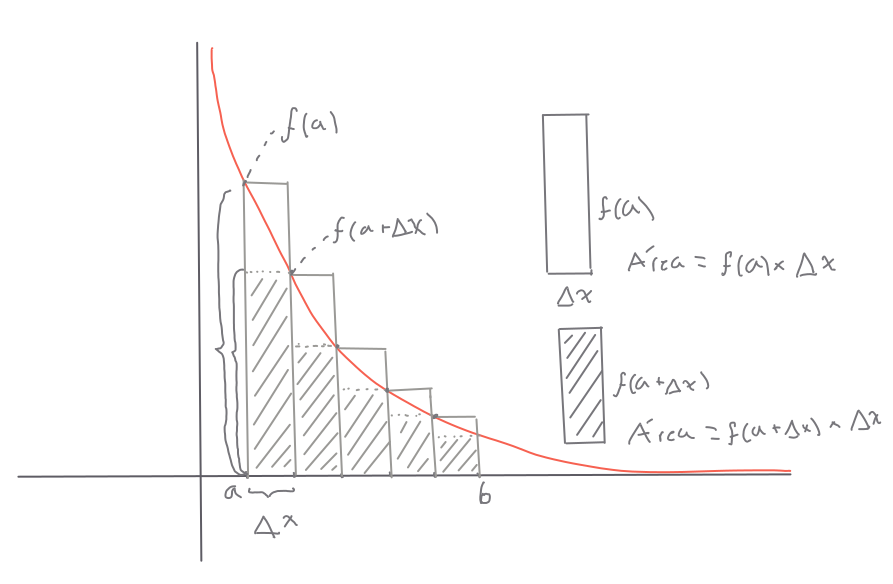
\includegraphics{Unidad-III/Esquema-integral} 

}

\caption{Representación esquemática de la integral. Nota quq utilizando los rectángulos, es posible aproximar el valor de una integral con rectángulos que pasen por arriba o abajo de la curva.}\label{fig:La-integral}
\end{figure}

Puedes explorar estos conceptos con la \href{https://www.geogebra.org/classic/wmpqmr4a}{aplicación para el área bajo una recta de Geogebra}.

\hypertarget{uxe1rea-bajo-una-recta}{%
\subsection{Área bajo una recta}\label{uxe1rea-bajo-una-recta}}

Un ejemplo clásico de integración es el área bajo una recta con pendiente \(m \neq 0\) e intercepto \(0\), la cual corresponde al área de un triángulo (figura \ref{fig:Area-recta}).

\begin{figure}

{\centering 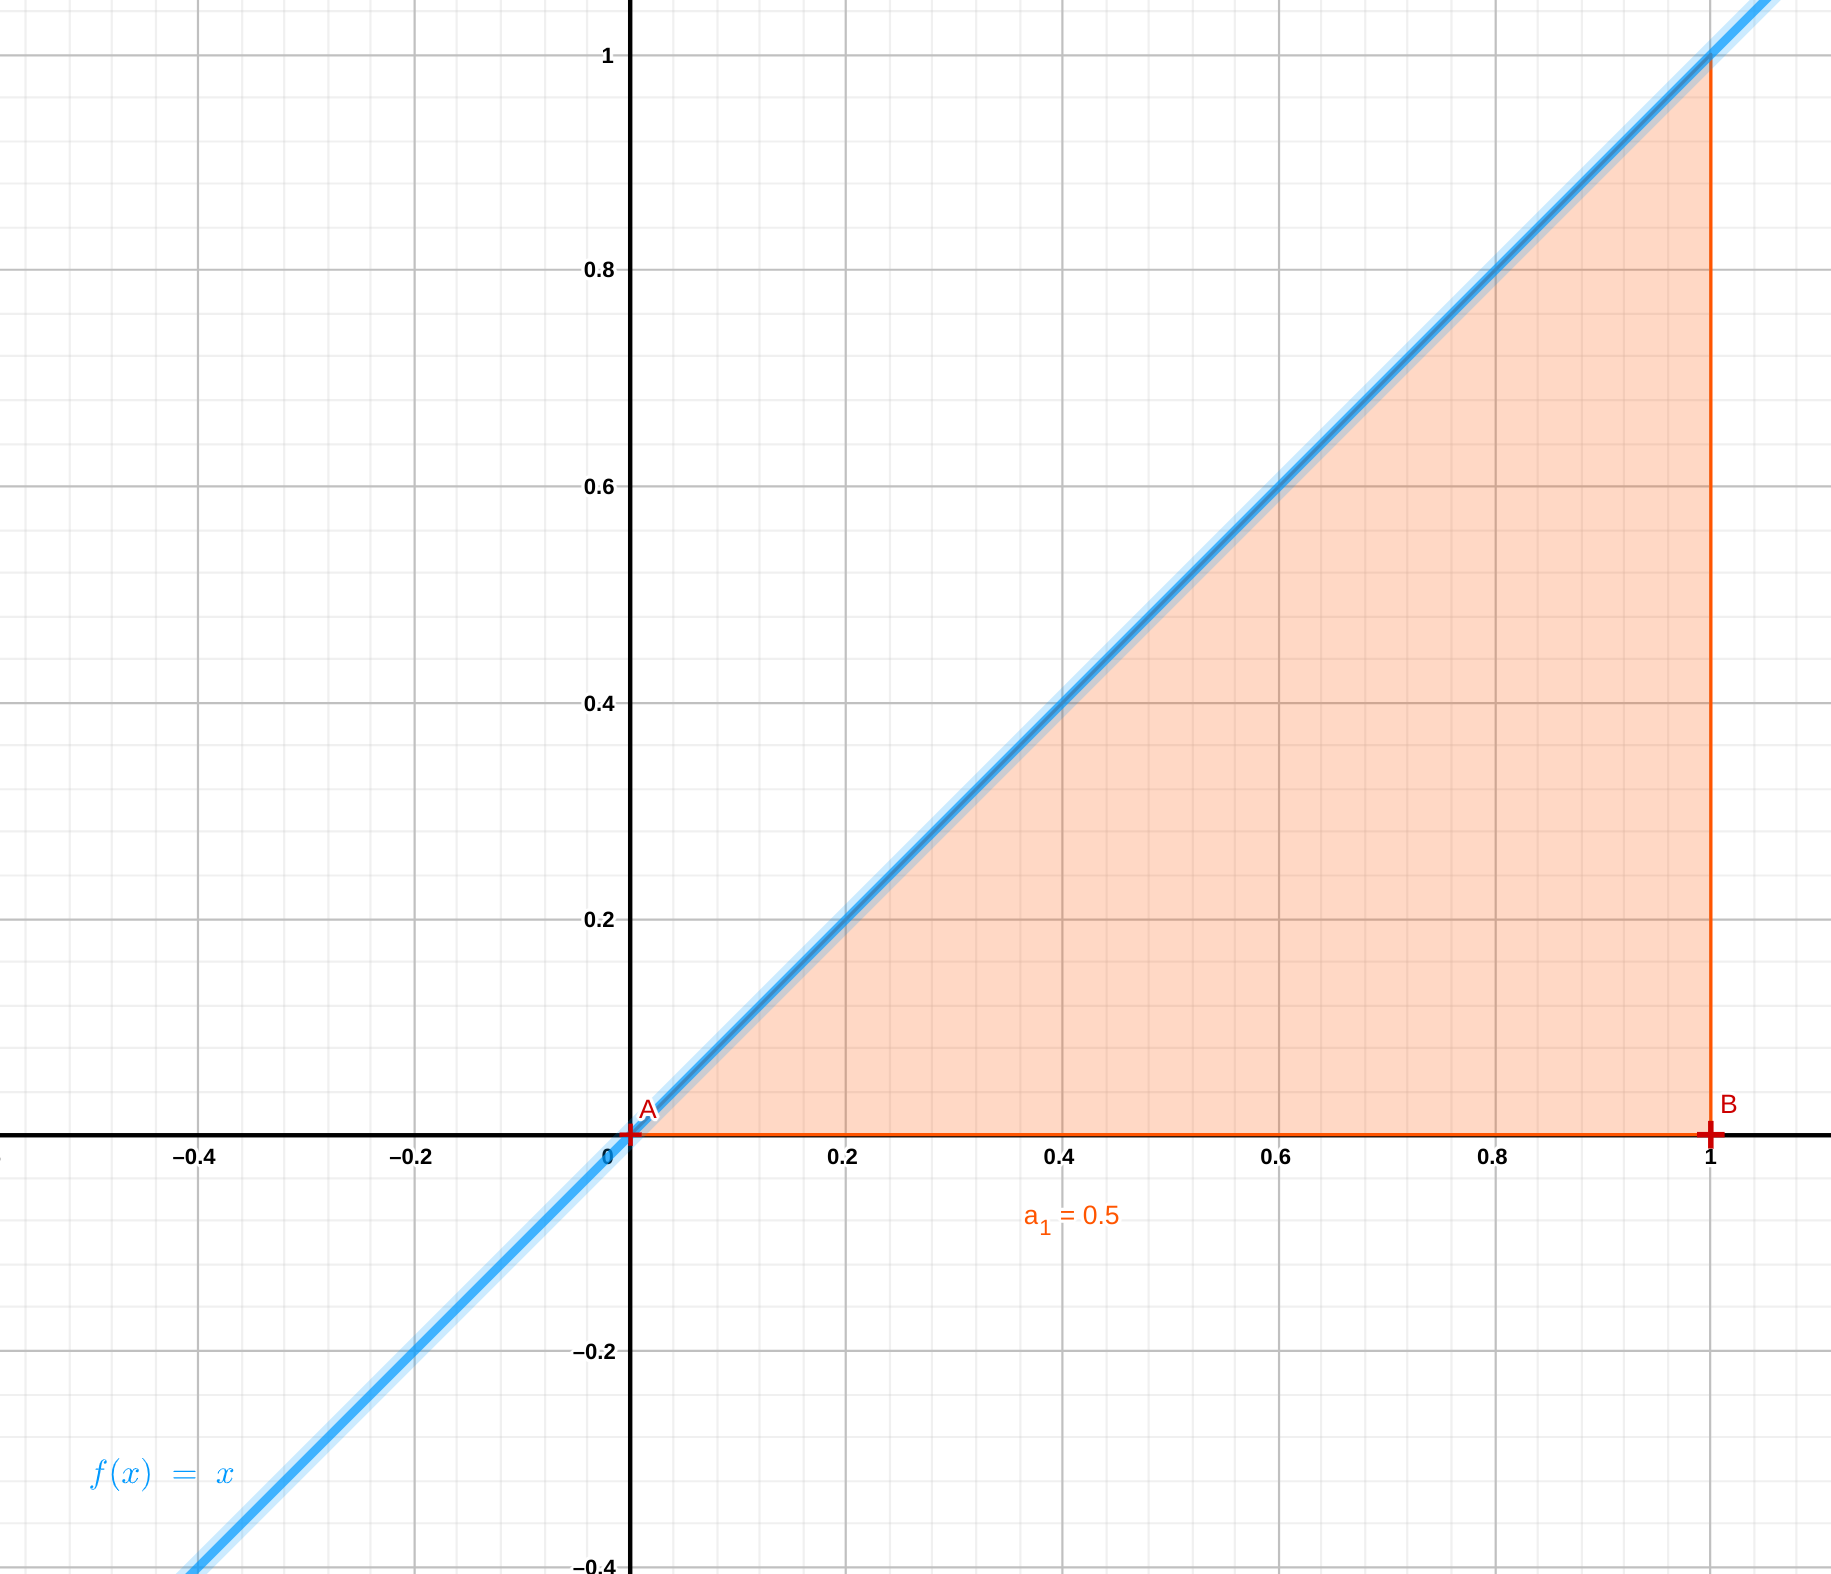
\includegraphics{Unidad-III/Area-bajo-recta} 

}

\caption{Área bajo la recta f(x) = x, entre el punto 0 y a = 1.}\label{fig:Area-recta}
\end{figure}

Utilizando el método de los rectángulos tenemos que el área sombreada en la figura \ref{fig:Area-recta} entre los puntos \(0\) y \(a\) se puede aproximar sumando rectángulos con altura \(f(x)\) y ancho \(\Delta x\).

\begin{figure}

{\centering 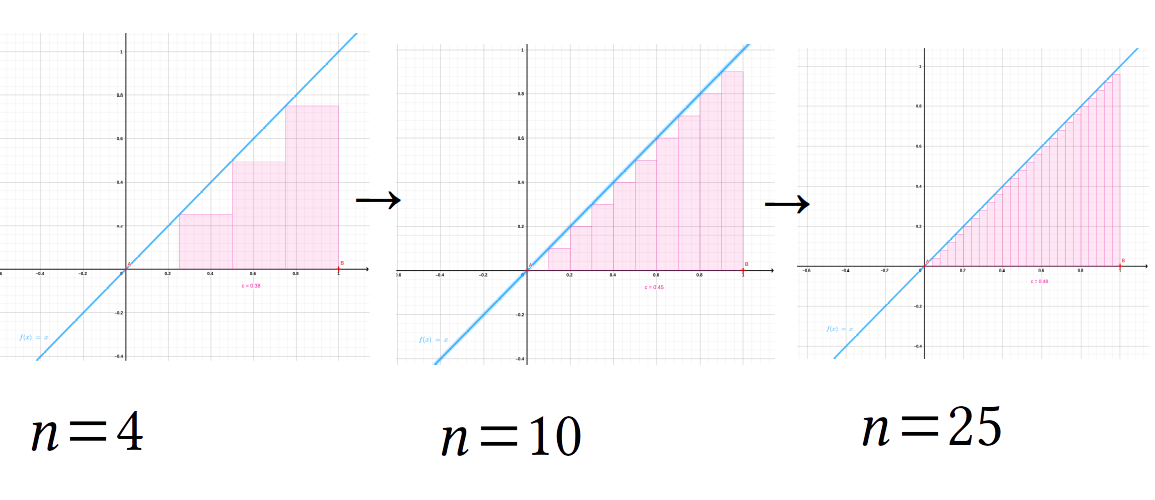
\includegraphics{Unidad-III/Rectangulos} 

}

\caption{Método de los rectángulos para calcular área bajo curva}\label{fig:Recta-area-rect}
\end{figure}

Para automatizar este proceso y encontrar todos los valores de \(x\) en el intervalo \(0, a\), podemos comenzar por tomar en cuenta el número de rectángulos, como en la figura \ref{fig:Recta-area-rect}, cuantos más rectángulos tenemos el error de cálculo será menor.

La siguiente consideración será si tomaremos en cuenta el punto inferior o superior del intervalo (figura \ref{fig:La-integral}). Si tomamos en cuenta el punto inferior del intervalo, la altura del primer rectángulo será \(f(0)\), y el ancho será \(\Delta x = a/n\). Por otra parte, tenemos que los valores de \(x\) en que evaluaremos \(f(x)\) corresponden a los valores de \(x: 0, a/n, 2a/n, 3a/n, \dots, (n-1)a/n, a\), Si comenzamos con \(n = 10\), y \(a = 1\) tenemos que evaluar \(f(x)\) en los valores:

\[x = \left \{ 0, \frac{1}{10}, \frac{1}{10}, \dots, \frac{9}{10}, 1 \right \}\]

Estas integrales se comoces como de Riemann. Por muchos años los matemáticos se dieron a la tarea de encontrar las funciones que resultaban de incremetar el número de rectángulos bajo la curva de diversas funciones. No fue sino hasta que Newton y Leibniz acuñaron el teorema fundamental del cálculo que se obtuvieron las herramientas necesarias para estimar \emph{fácilmente} el ára bajo la curva de cualquier función.

\textbf{De aquí en adelante está en construcción, no usar!}

\hypertarget{el-teorema-funamental-del-cuxe1lculo}{%
\subsection{El teorema funamental del cálculo}\label{el-teorema-funamental-del-cuxe1lculo}}

Este teorema establece, en términos muy generales que

\begin{equation}
\int \frac{d}{dx}f = f(x)
\end{equation}

la integral de una derivada es la función misma con la que se obtuvo la derivada. Así, llegamos a la antiderivada.

\hypertarget{antiderivadas-de-funciones}{%
\subsubsection{Antiderivadas de funciones}\label{antiderivadas-de-funciones}}

Bajo la regla de las potencias, que si \(f(x) = ax^n\), \(\int f(x) = \frac{ax^{n+1}}{n+1}\). Si derivamos \(\int f(x)\), veremos que \(f(x) = ax^n\).

Esta sencillísima técnica es efectiva para funciones sin constantes, puesto que la derivada de una constante es 0. Sin embargo debido a que al integrar una función no tenemos ningún conocimiento sobre la existencia o ausencia de una constante (p.~ej. \(y = a + bx\)), es necesario asumir su existencia, de modo que:

\begin{equation}
\int f(x) = \frac{ax^{n+1}}{n+1} + c
\end{equation}

donde \(c\) es la constante de integración.

\hypertarget{aplicaciones-de-la-integraciuxf3n}{%
\subsection{Aplicaciones de la integración}\label{aplicaciones-de-la-integraciuxf3n}}

\hypertarget{cambio-acumulativo}{%
\subsubsection{Cambio acumulativo}\label{cambio-acumulativo}}

El modelo de crecimiento exponencial, basado en la ecuación:

\begin{equation}
    N(t) = e^{rt} \label{eq:ExponN}
\end{equation}

es la base de un gran número de modelos en ecología. Cuando transformamos este modelo en una ecuación diferencial, toma una apariencia un tanto diferente. Comencemos por recordar que si \(f(x) = e^x\), entonces \(f'(x) = e^x\). Si agregamos un parámetro \(r\) como coeficiente de \(x\), tenemos que \(f(x)= e^{rx}\), resultando exactamente en el modelo \eqref{eq:ExponN}.

Para derivar este modelo necesitamos recordar que:

\[\frac{d}{dx}(f \circ g)(x) = (f \circ g)'(x)g'(x)\]
y por analogía \((f \circ g)(x) = e^{rt}\) y \(g(x) = rt\), por lo tanto:

\begin{equation}
\frac{dN}{dt} = r e^{rt}
\end{equation}

donde podemos sustituir \(e^{rt}\) por \(N\), para obtener:

\begin{equation}
\frac{dN}{dt} = r N
\end{equation}

que el cambio inmediato en el número de individuos de la población \(N\), es proporcional a \(rN\). La integral \(\int_{0}^{t} \frac{dN}{dt}\) es entonces equivalente al número de individuos en ese momento \(t\), mientras que \(\int_{0}^{t} N(t)\) corresponde al número total de individuos que hay y ha habido en esa población!

\hypertarget{integraciuxf3n-analuxedtica-vs-numuxe9rica}{%
\subsubsection{Integración analítica vs numérica}\label{integraciuxf3n-analuxedtica-vs-numuxe9rica}}

En matemáticas, el término \emph{analítico} se utiliza para describir el proceso de encontrar con herramientas formales de las matemáticas una solución exacta a un problema. Por ejemplo la antiderivación, aplicando a la inversa las relgas de la derivación es la integración analítica. Hay modelos sin embargo que no se pueden resolver con herramientas analíticas, típicamente, aquellos en que no podemos separar las variables dependientes e independientes. En esos casos hacemos integración \emph{numérica}, que consiste en aproximaciones al valor de la función pero nunca representan las soluciones exactas que se obtienen con integración analítica.

Veamos la ecuación diferencial:

\begin{equation}
\frac{dN}{dt} = rN \label{eq:dif-1}
\end{equation}

corresponde a una función que conocemos como \(N = e^{rt}\), sin embargo podríamos aproximarnos recursivamente a los valores que prediciría \(e^{rt}\) utilizando la definición de la derivada. Sabemos que la derivada es la pendiente de una recta, por lo tanto podríamos comenzar por dibujar una recta con pendiente \(rN\) partiendo desde \(t = 0\), hasta un punto \(0+dx\). El cambio absoluto de \(N\) (\(dN\)) sería entonces \(rN \times dt\), cuyo valorr utilizaremos como punto de partida. Mencioné anteriormente que este método es una aproximación, y esto es porque resulta en un error que se va acumulando entre la función verdadera \(N = e^{rt}\) y la que aproximamos revirtiendo secuencialmente la derivada (figura ).

\begin{figure}

{\centering 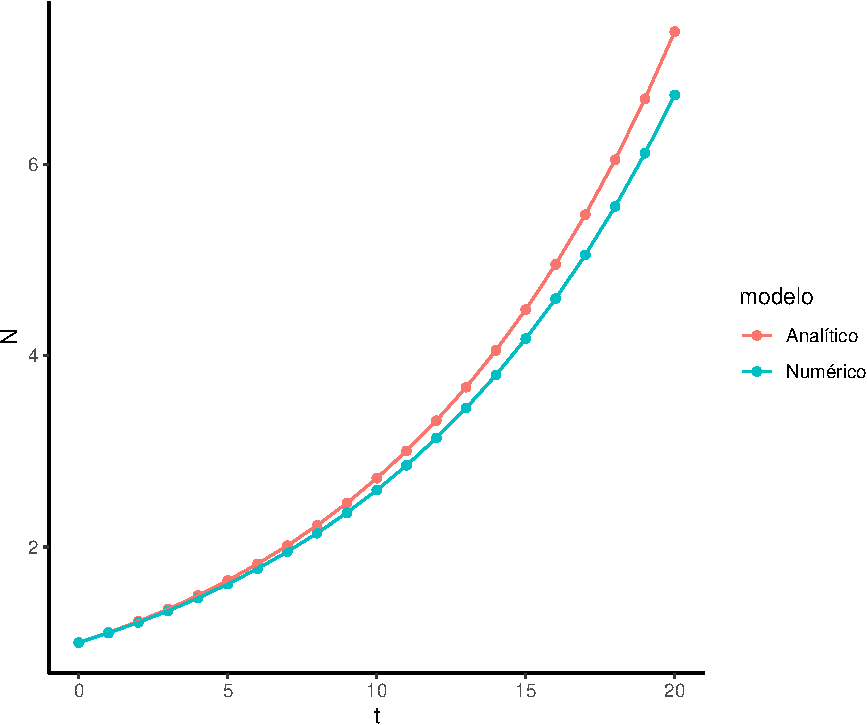
\includegraphics{Model-mate_files/figure-latex/integ-numer-1} 

}

\caption{Diferencias entre integración analítica vs integración numérica, para r = 0.1, dt = 1, y población inicial de N = 1.}\label{fig:integ-numer}
\end{figure}

  \bibliography{book.bib,packages.bib}

\end{document}
